% filename: ProgramPlots1.tex
\documentclass[11pt]{article}
\include{PhysNote}
\usepackage{srcltx}

\usepackage{ifpdf} % to switch between .eps and .png file types for images (for compiling)


\title{Program Plots 1}
\author{Andrew Forrester}


\begin{document}
\maketitle
\tableofcontents


\newpage
\section{Files}

\begin{comment}
plot_a0VsTP.ps
plot_HeatCapVsTemp_DK0050.ps
plot_HeatCapVsTemp.ps
plot_HeatCapVsTempV_b.ps
plot_HeatCapVsTempV_DK0030.ps
plot_HeatCapVsTempV_DK0040.ps
plot_HeatCapVsTempV_DK0050.ps
plot_HeatCapVsTempV_DK0060.ps
plot_HeatCapVsTempV_DK0070.ps
plot_HeatCapVsTempV_DK0080.ps
plot_HeatCapVsTempV_DK0090.ps
plot_HeatCapVsTempV_DK0100.ps
plot_HeatCapVsTempV_DK0110.ps
plot_HeatCapVsTempV_DK0120.ps
plot_HeatCapVsTempV_DK0130.ps
plot_HeatCapVsTempV_DK0140.ps
plot_HeatCapVsTempV.ps
plot_HeatCapVsTvPress.ps
plot.ps
plot_vlt_HeatCap_P_DK0_1e-07_CapVsTv_log_AhlersCompare_adjust.ps
plot_vlt_HeatCap_P_DK0_1e-07_CapVsTv_log_AhlersCompare.ps
plot_vlt_HeatCap_P_DK0_1e-07_CapVsTv_log.ps
plot_vlt_HeatCap_P_DK0_1e-07_CapVsTv.ps
plot_vlt_ThermStates_Dexp100_A_RhosoRhoVsTvNu.ps
splot_a0VsTP.ps

plot_2D_KrK0versusl_B_linlin.png
plot_2D_KrK0versusT_B_linlin.png
plot_2D_KrversusT_A_linlin.png
plot_2D_KrversusT_B_linlin.png
plot_2D_Kversusl_A_loglin.png
plot_2D_Kversusl_B_linlin.png
plot_2D_yversusl_B_loglin.png
plot_2D_yversusT_B_loglin.png
plot_3D_Fversusl_B_linlin.png
plot_3D_FversusT_B_linlin.png
plot_3D_KrK0versusl_A_loglog.png
plot_3D_KrK0versusl_B_linlin.png
plot_3D_KrK0versusl_B_loglog.png
plot_3D_KrK0versusT_B_linlin.png
plot_3D_KrK0versusTv_A_findA.png
plot_3D_KrK0versusTv_A_loglog.png
plot_3D_KrK0versusTv_B_findA.png
plot_3D_KrK0versusTv_B_loglog.png
plot_3D_KrversusT_B_linlin.png
plot_3D_Kversusl_A_loglin.png
plot_3D_Kversusl_A_loglog.png
plot_3D_Kversusl_B_linlin.png
plot_3D_yversusl_A_loglog.png
plot_3D_yversusl_B_linlin.png
plot_3D_yversusT_B_linlin.png
plot_rhos_compare_alpha.png
plot_rhos_compare_beta.png
plot_ring3_A_KrK0versusTv.png
plot_ring3_A_rhosAmps.png
plot_ring3_Delok_alpha.png
plot_ring3_Delok_beta.png
\end{comment}


\squishlist
  \item PostScript (.ps)
	\squishlisti
	  \item \verb|plot_a0VsTP.ps|
	  \item \verb|plot_HeatCapVsTemp_DK0050.ps|
	  \item \verb|plot_HeatCapVsTemp.ps|
	  \item \verb|plot_HeatCapVsTempV_b.ps|
	  \item \verb|plot_HeatCapVsTempV_DK0030.ps|
	  \item \verb|plot_HeatCapVsTempV_DK0040.ps|
	  \item \verb|plot_HeatCapVsTempV_DK0050.ps|
	  \item \verb|plot_HeatCapVsTempV_DK0060.ps|
	  \item \verb|plot_HeatCapVsTempV_DK0070.ps|
	  \item \verb|plot_HeatCapVsTempV_DK0080.ps|
	  \item \verb|plot_HeatCapVsTempV_DK0090.ps|
	  \item \verb|plot_HeatCapVsTempV_DK0100.ps|
	  \item \verb|plot_HeatCapVsTempV_DK0110.ps|
	  \item \verb|plot_HeatCapVsTempV_DK0120.ps|
	  \item \verb|plot_HeatCapVsTempV_DK0130.ps|
	  \item \verb|plot_HeatCapVsTempV_DK0140.ps|
	  \item \verb|plot_HeatCapVsTempV.ps|
	  \item \verb|plot_HeatCapVsTvPress.ps|
	  \item \verb|plot.ps|
	  \item \verb|plot_vlt_HeatCap_P_DK0_1e-07_CapVsTv_log_AhlersCompare_adjust.ps|
	  \item \verb|plot_vlt_HeatCap_P_DK0_1e-07_CapVsTv_log_AhlersCompare.ps|
	  \item \verb|plot_vlt_HeatCap_P_DK0_1e-07_CapVsTv_log.ps|
	  \item \verb|plot_vlt_HeatCap_P_DK0_1e-07_CapVsTv.ps|
	  \item \verb|plot_vlt_ThermStates_Dexp100_A_RhosoRhoVsTvNu.ps|
	  \item \verb|splot_a0VsTP.ps|
	\squishend
  \item Portable Network Graphics (.png)
	\squishlisti
	  \item \verb|plot_2D_KrK0versusl_B_linlin.png|
	  \item \verb|plot_2D_KrK0versusT_B_linlin.png|
	  \item \verb|plot_2D_KrversusT_A_linlin.png|
	  \item \verb|plot_2D_KrversusT_B_linlin.png|
	  \item \verb|plot_2D_Kversusl_A_loglin.png|
	  \item \verb|plot_2D_Kversusl_B_linlin.png|
	  \item \verb|plot_2D_yversusl_B_loglin.png|
	  \item \verb|plot_2D_yversusT_B_loglin.png|
	  \item \verb|plot_3D_Fversusl_B_linlin.png|
	  \item \verb|plot_3D_FversusT_B_linlin.png|
	  \item \verb|plot_3D_KrK0versusl_A_loglog.png|
	  \item \verb|plot_3D_KrK0versusl_B_linlin.png|
	  \item \verb|plot_3D_KrK0versusl_B_loglog.png|
	  \item \verb|plot_3D_KrK0versusT_B_linlin.png|
	  \item \verb|plot_3D_KrK0versusTv_A_findA.png|
	  \item \verb|plot_3D_KrK0versusTv_A_loglog.png|
	  \item \verb|plot_3D_KrK0versusTv_B_findA.png|
	  \item \verb|plot_3D_KrK0versusTv_B_loglog.png|
	  \item \verb|plot_3D_KrversusT_B_linlin.png|
	  \item \verb|plot_3D_Kversusl_A_loglin.png|
	  \item \verb|plot_3D_Kversusl_A_loglog.png|
	  \item \verb|plot_3D_Kversusl_B_linlin.png|
	  \item \verb|plot_3D_yversusl_A_loglog.png|
	  \item \verb|plot_3D_yversusl_B_linlin.png|
	  \item \verb|plot_3D_yversusT_B_linlin.png|
	  \item \verb|plot_rhos_compare_alpha.png|
	  \item \verb|plot_rhos_compare_beta.png|
	  \item \verb|plot_ring3_A_KrK0versusTv.png|
	  \item \verb|plot_ring3_A_rhosAmps.png|
	  \item \verb|plot_ring3_Delok_alpha.png|
	  \item \verb|plot_ring3_Delok_beta.png|
	\squishend
\squishend



\section{Data Fit}

This is actually Tc versus P:
\begin{center}
\begin{tabular}[\textwidth]{p{.5\textwidth}p{.5\textwidth}}
\ifpdf
  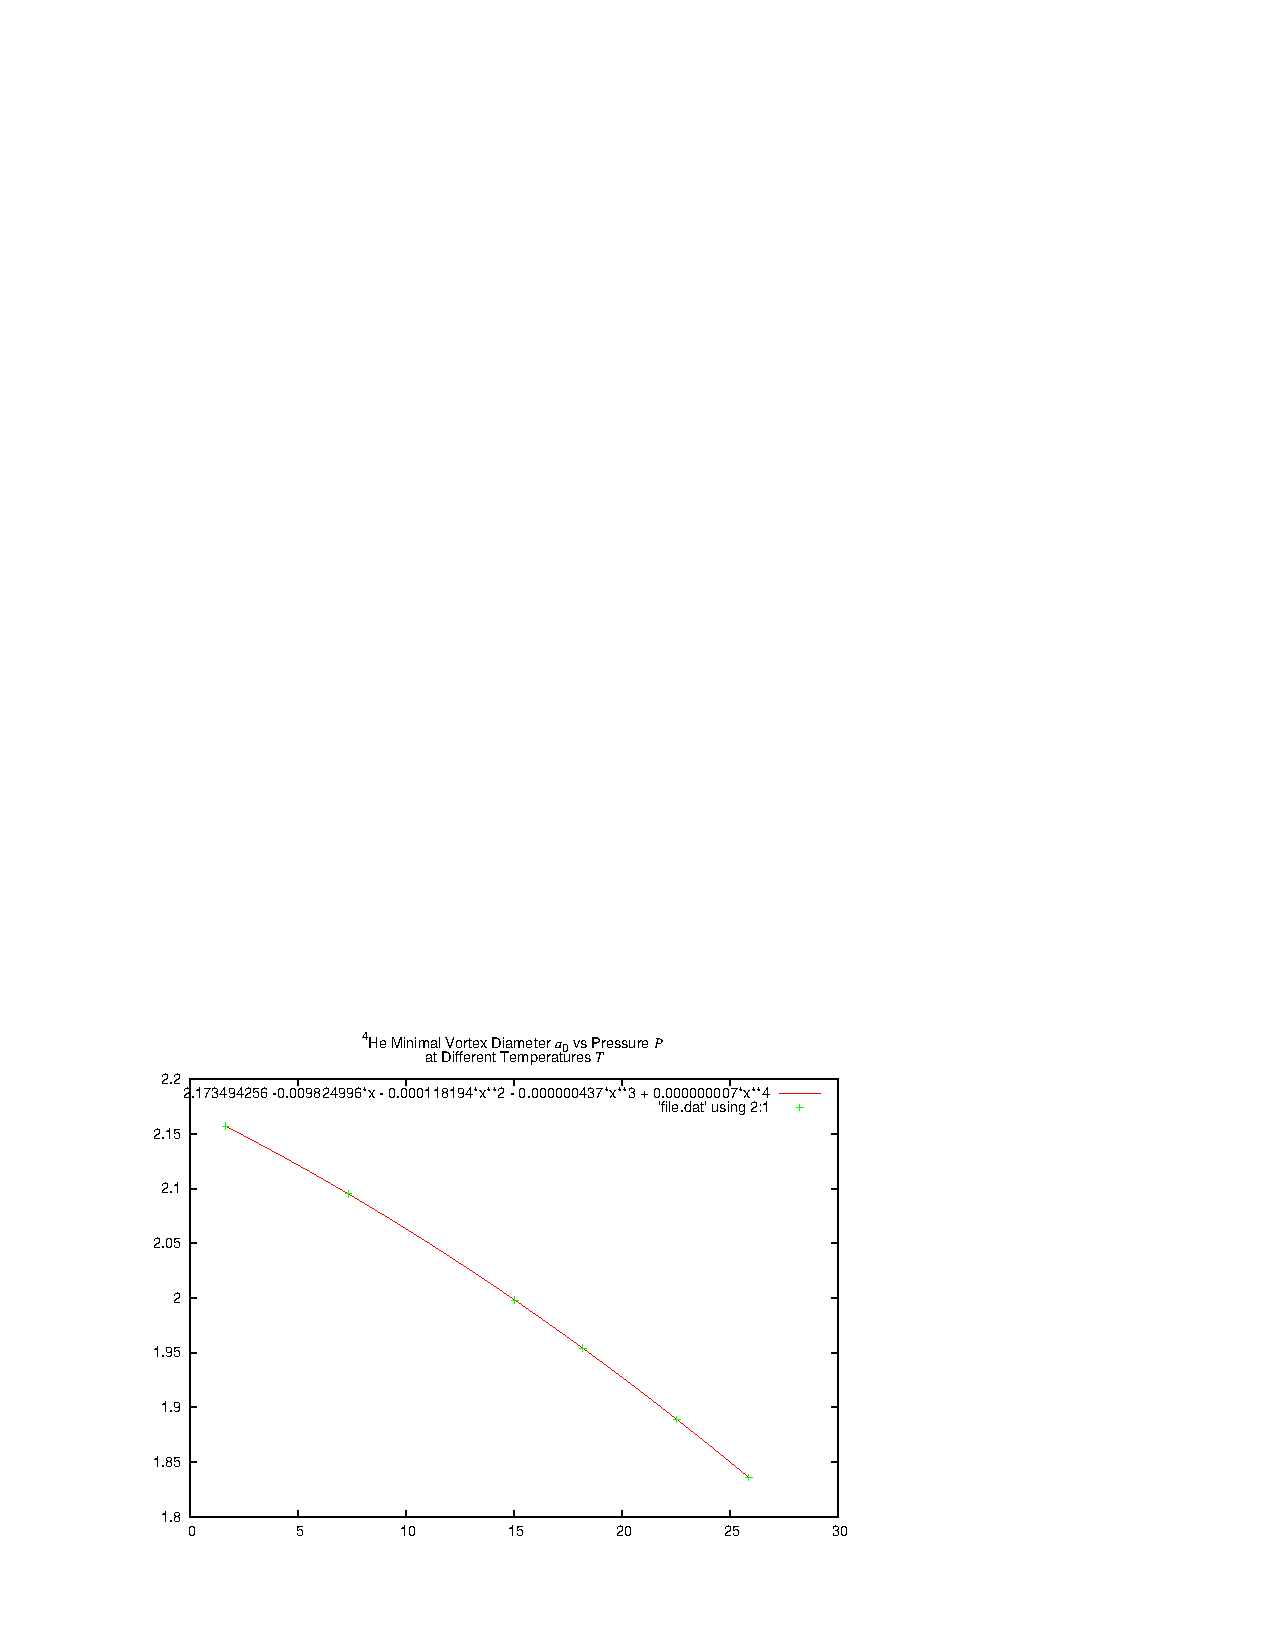
\includegraphics[width=8.5cm,viewport=54 53 410 300]{plot.pdf}\newline
  \verb|plot.pdf|
\else
  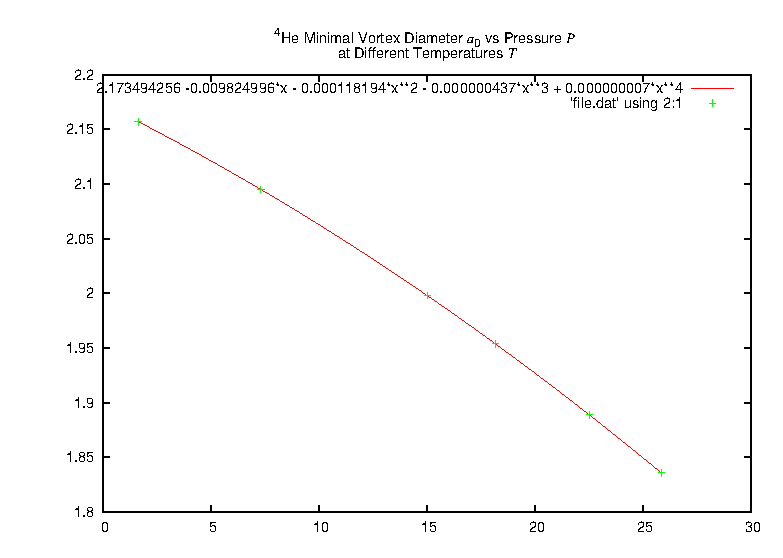
\includegraphics[width=8.5cm]{plot.ps}\newline
  \verb|plot.ps|
\fi
&
 \\
\end{tabular}
\end{center}



\section{Plots before Correction of K0cFind Program}

\begin{center}
\begin{tabular}[\textwidth]{p{.5\textwidth}p{.5\textwidth}}
\ifpdf
  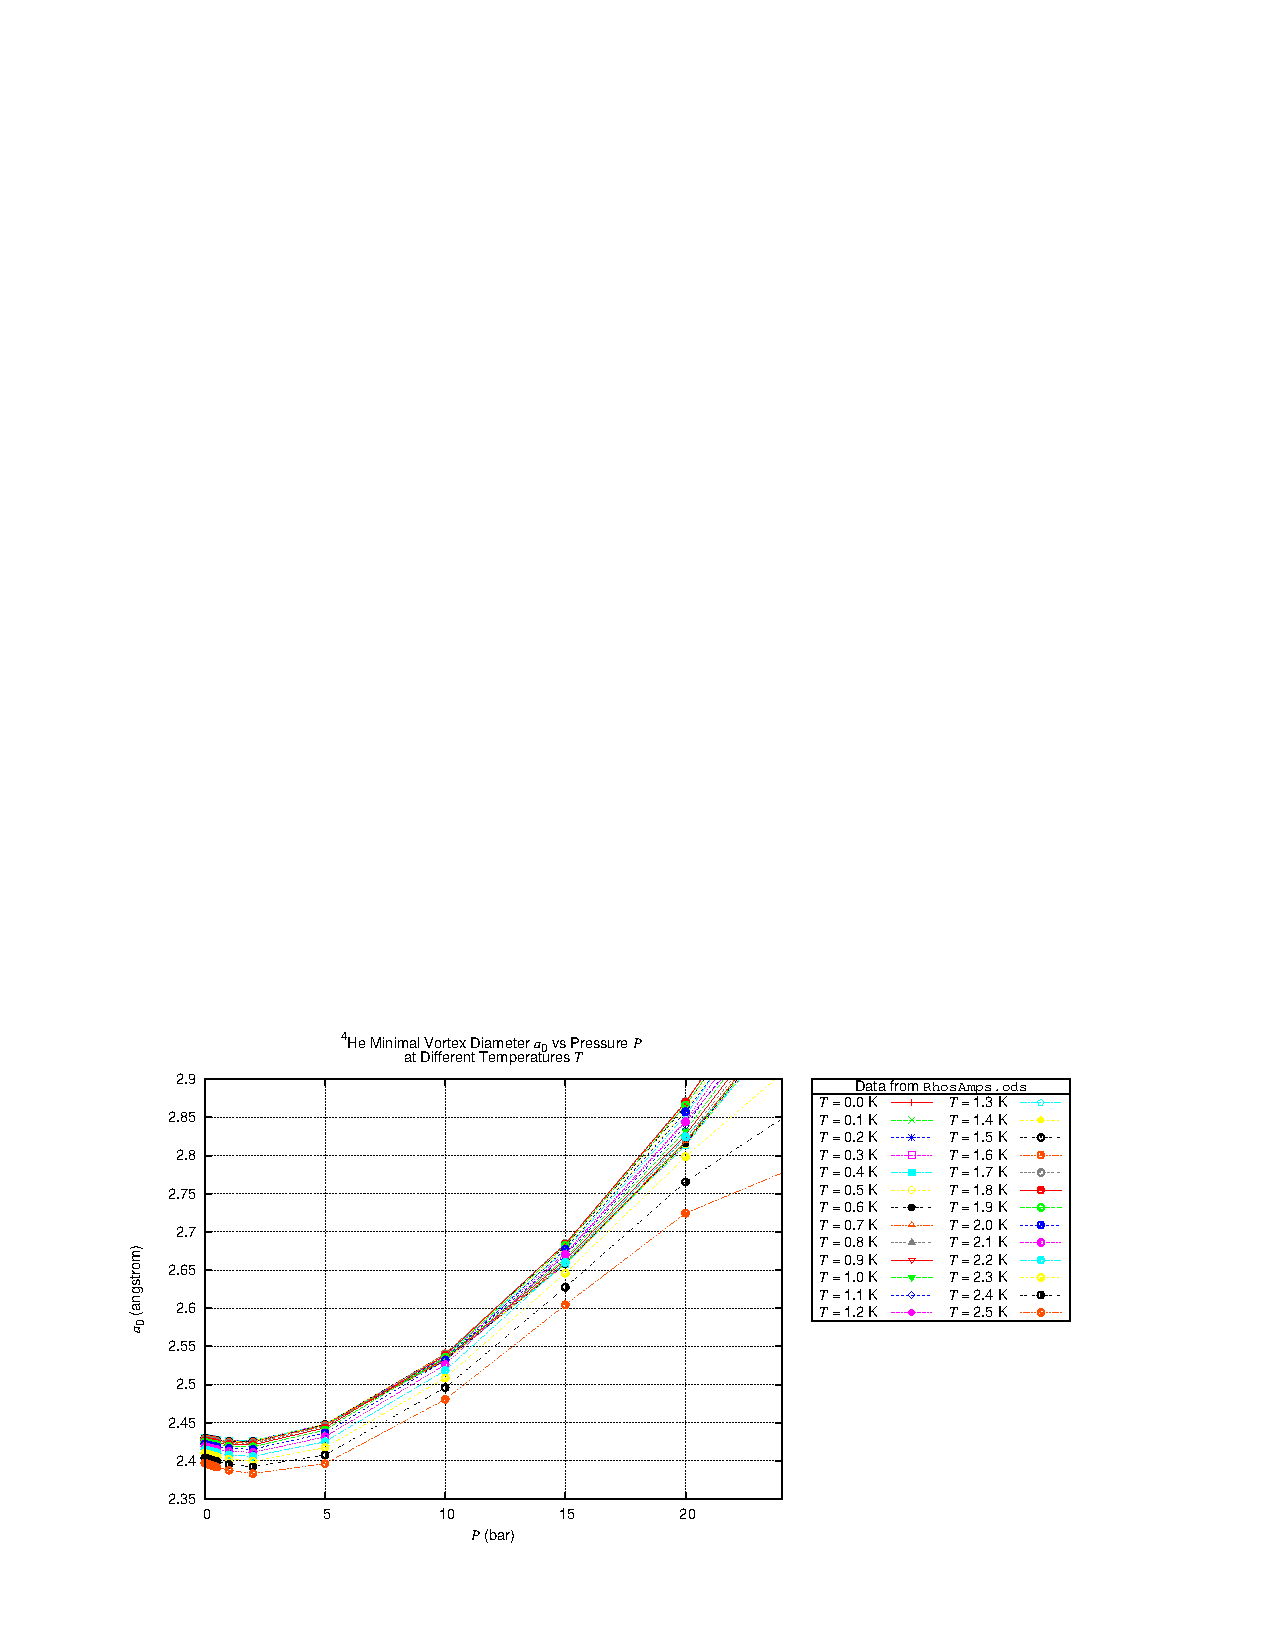
\includegraphics[width=8.5cm,viewport=54 53 410 300]{plot_a0VsTP.pdf}\newline
  \verb|plot_a0VsTP.pdf|
\else
  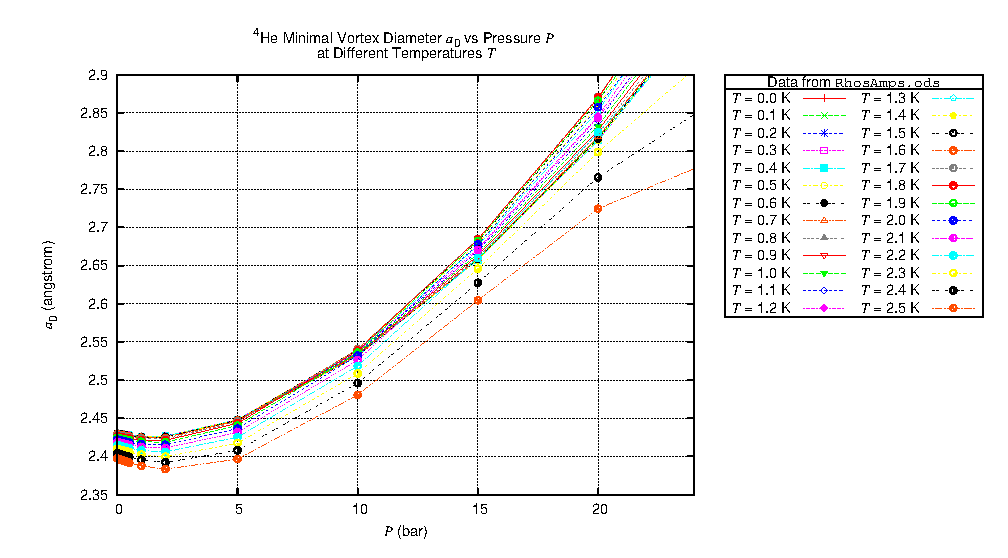
\includegraphics[width=8.5cm]{plot_a0VsTP.ps}\newline
  \verb|plot_a0VsTP.ps|
\fi
&
\ifpdf
  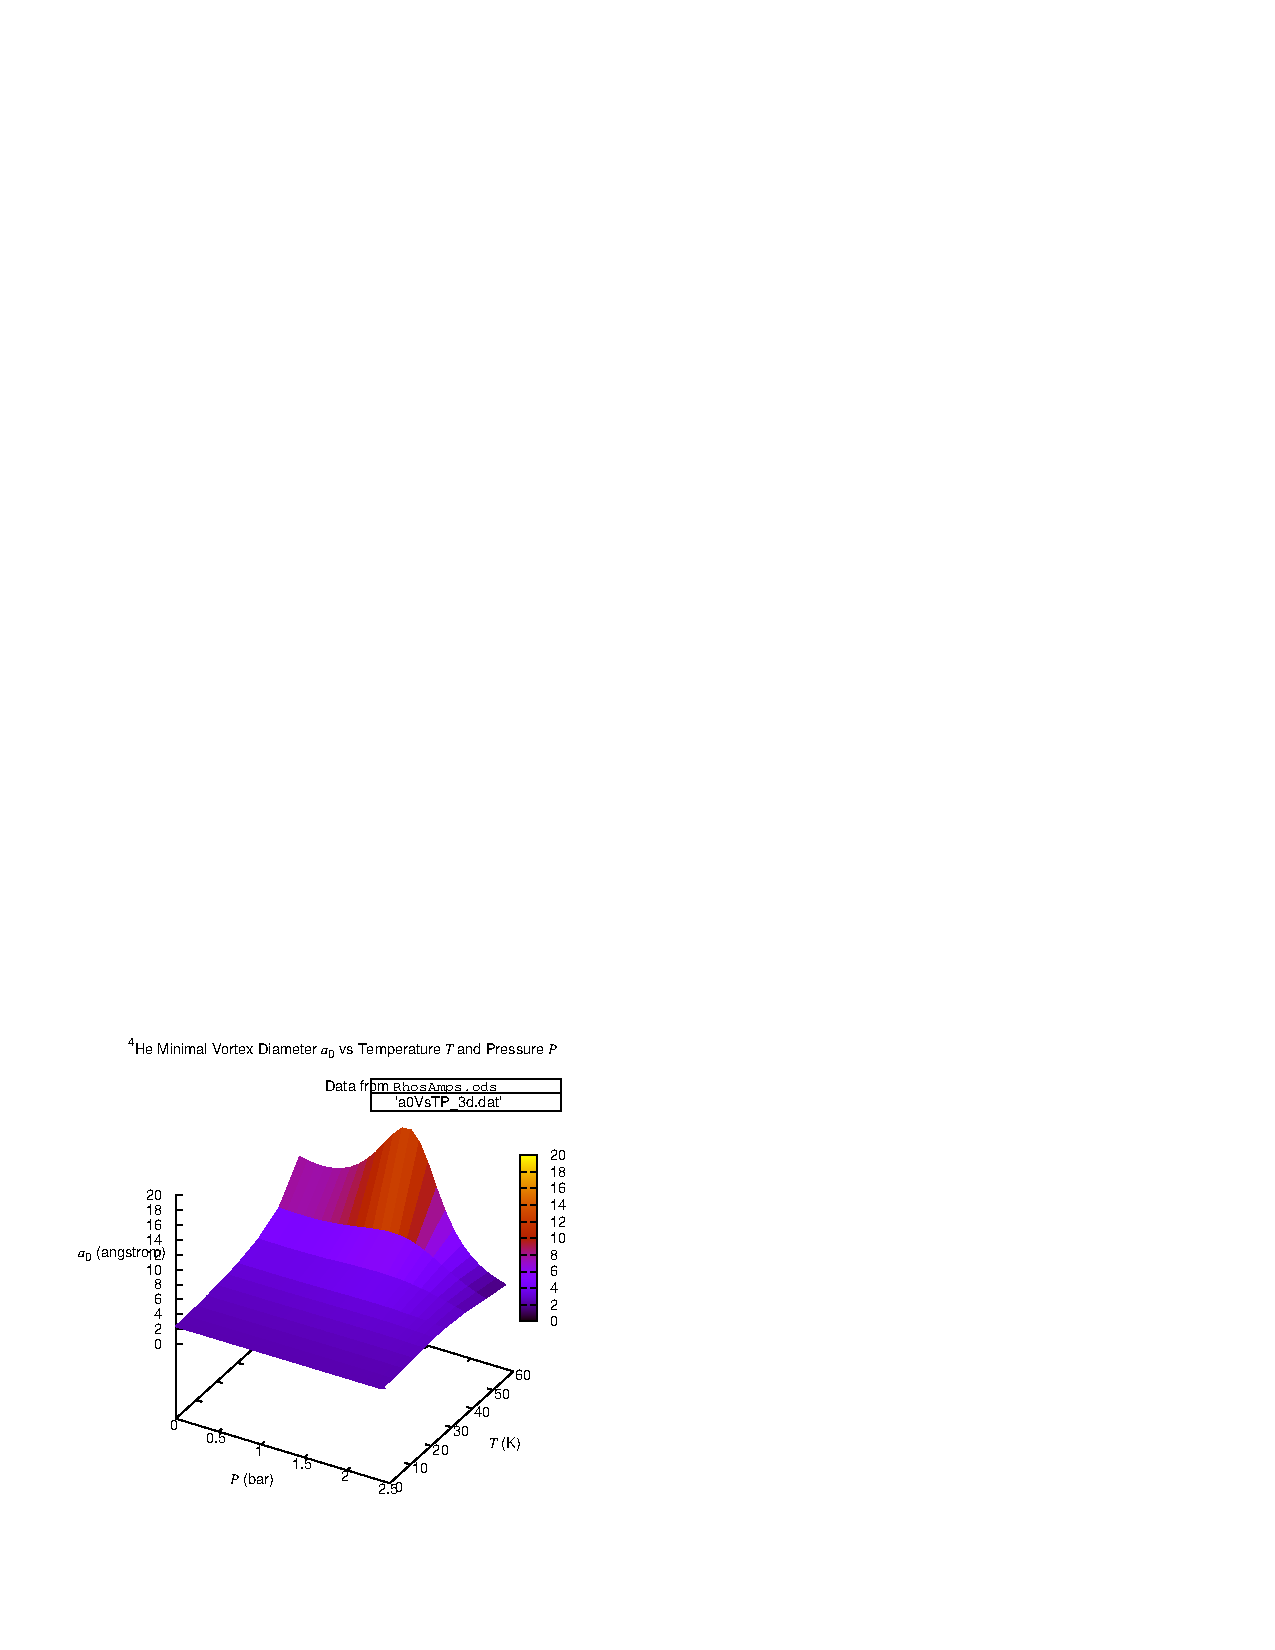
\includegraphics[width=6cm,viewport=-60 60 200 200]{splot_a0VsTP.pdf}\newline
  \vspace{10pt}\verb|splot_a0VsTP.pdf|
\else
  \includegraphics[width=8.5cm]{splot_a0VsTP.ps}\newline
  \verb|splot_a0VsTP.ps|
\fi
 \\
\end{tabular}
\end{center}


\begin{tabular}[\textwidth]{p{8.5cm}p{8.5cm}}
\ifpdf
  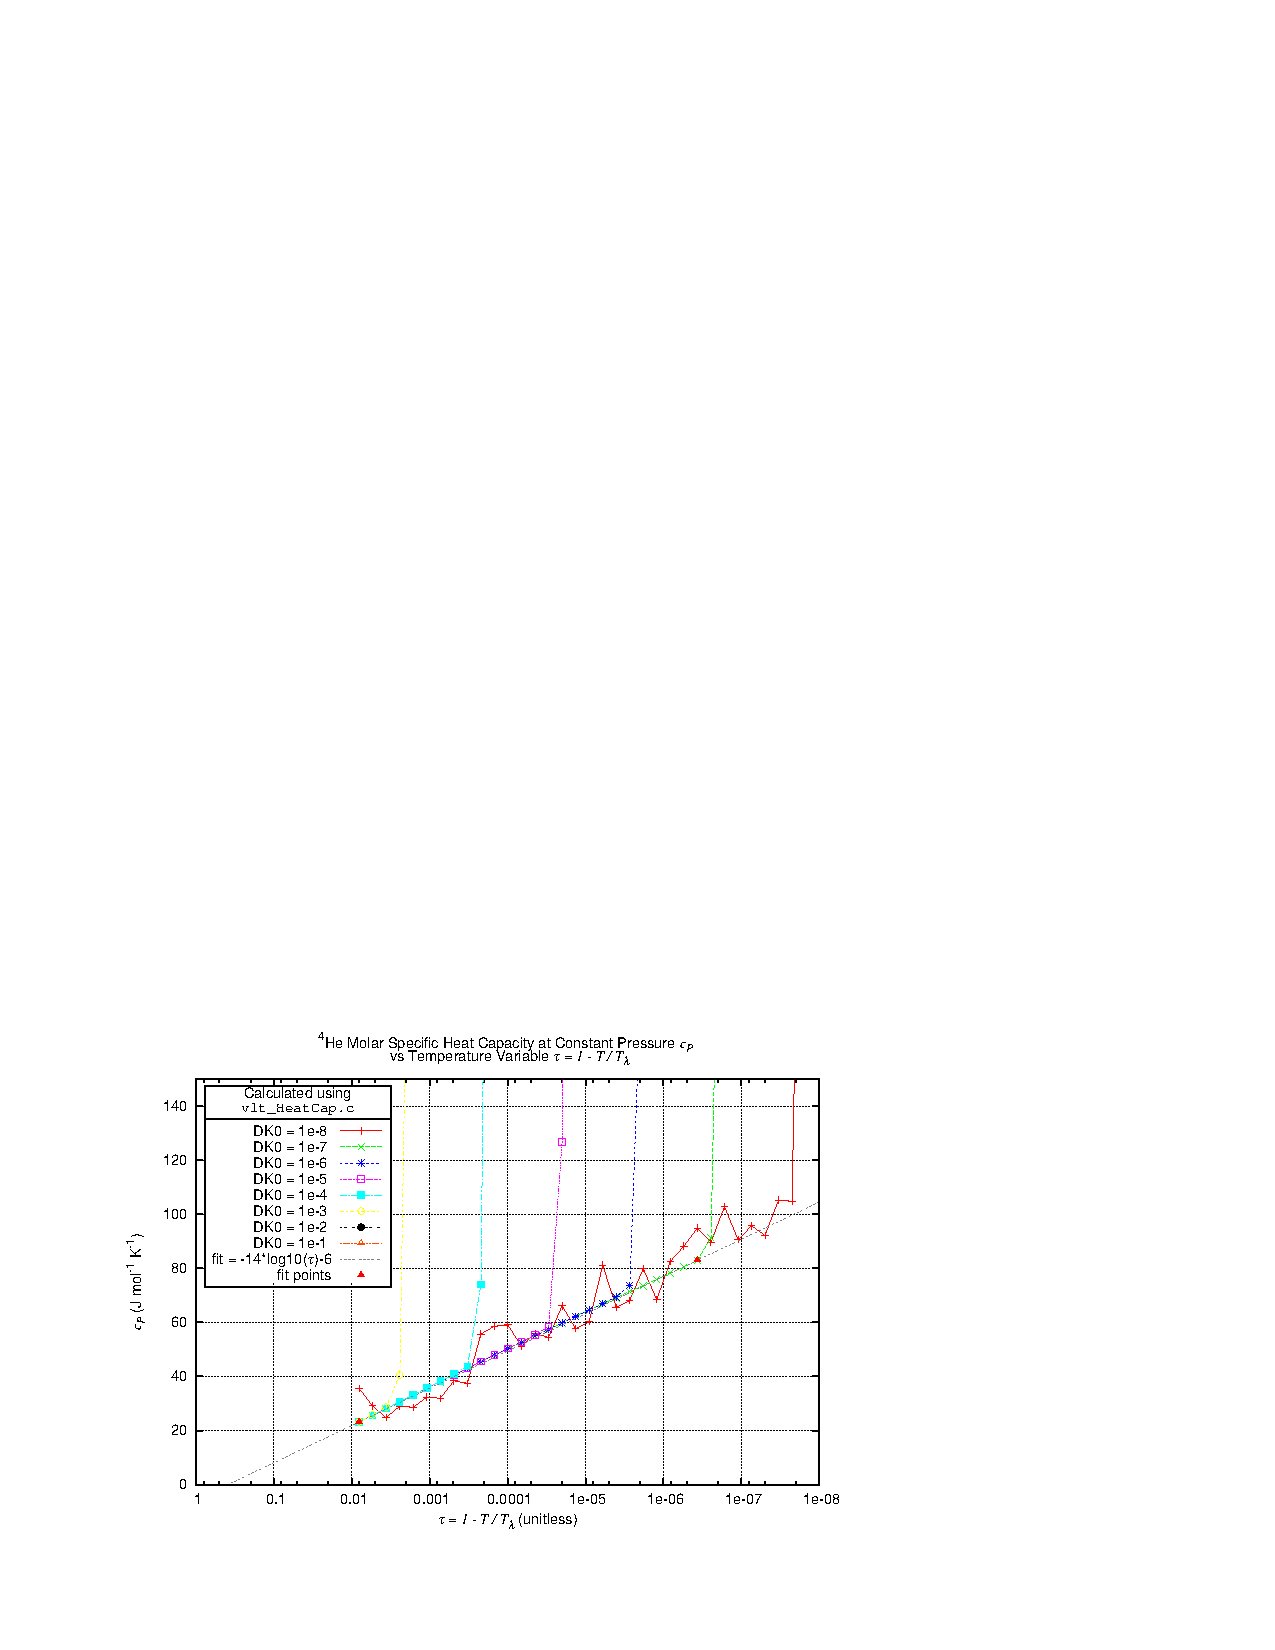
\includegraphics[width=8.5cm,viewport=54 53 410 300]{plot_HeatCapVsTempV.pdf}\newline
  \verb|plot_HeatCapVsTempV.pdf|
\else
  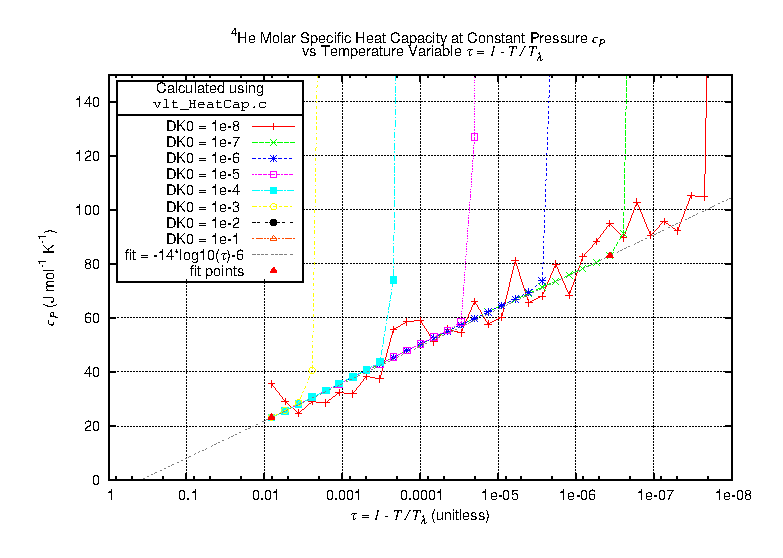
\includegraphics[width=8.5cm]{plot_HeatCapVsTempV.ps}\newline
  \verb|plot_HeatCapVsTempV.ps|
\fi
&
 \\
\ifpdf
  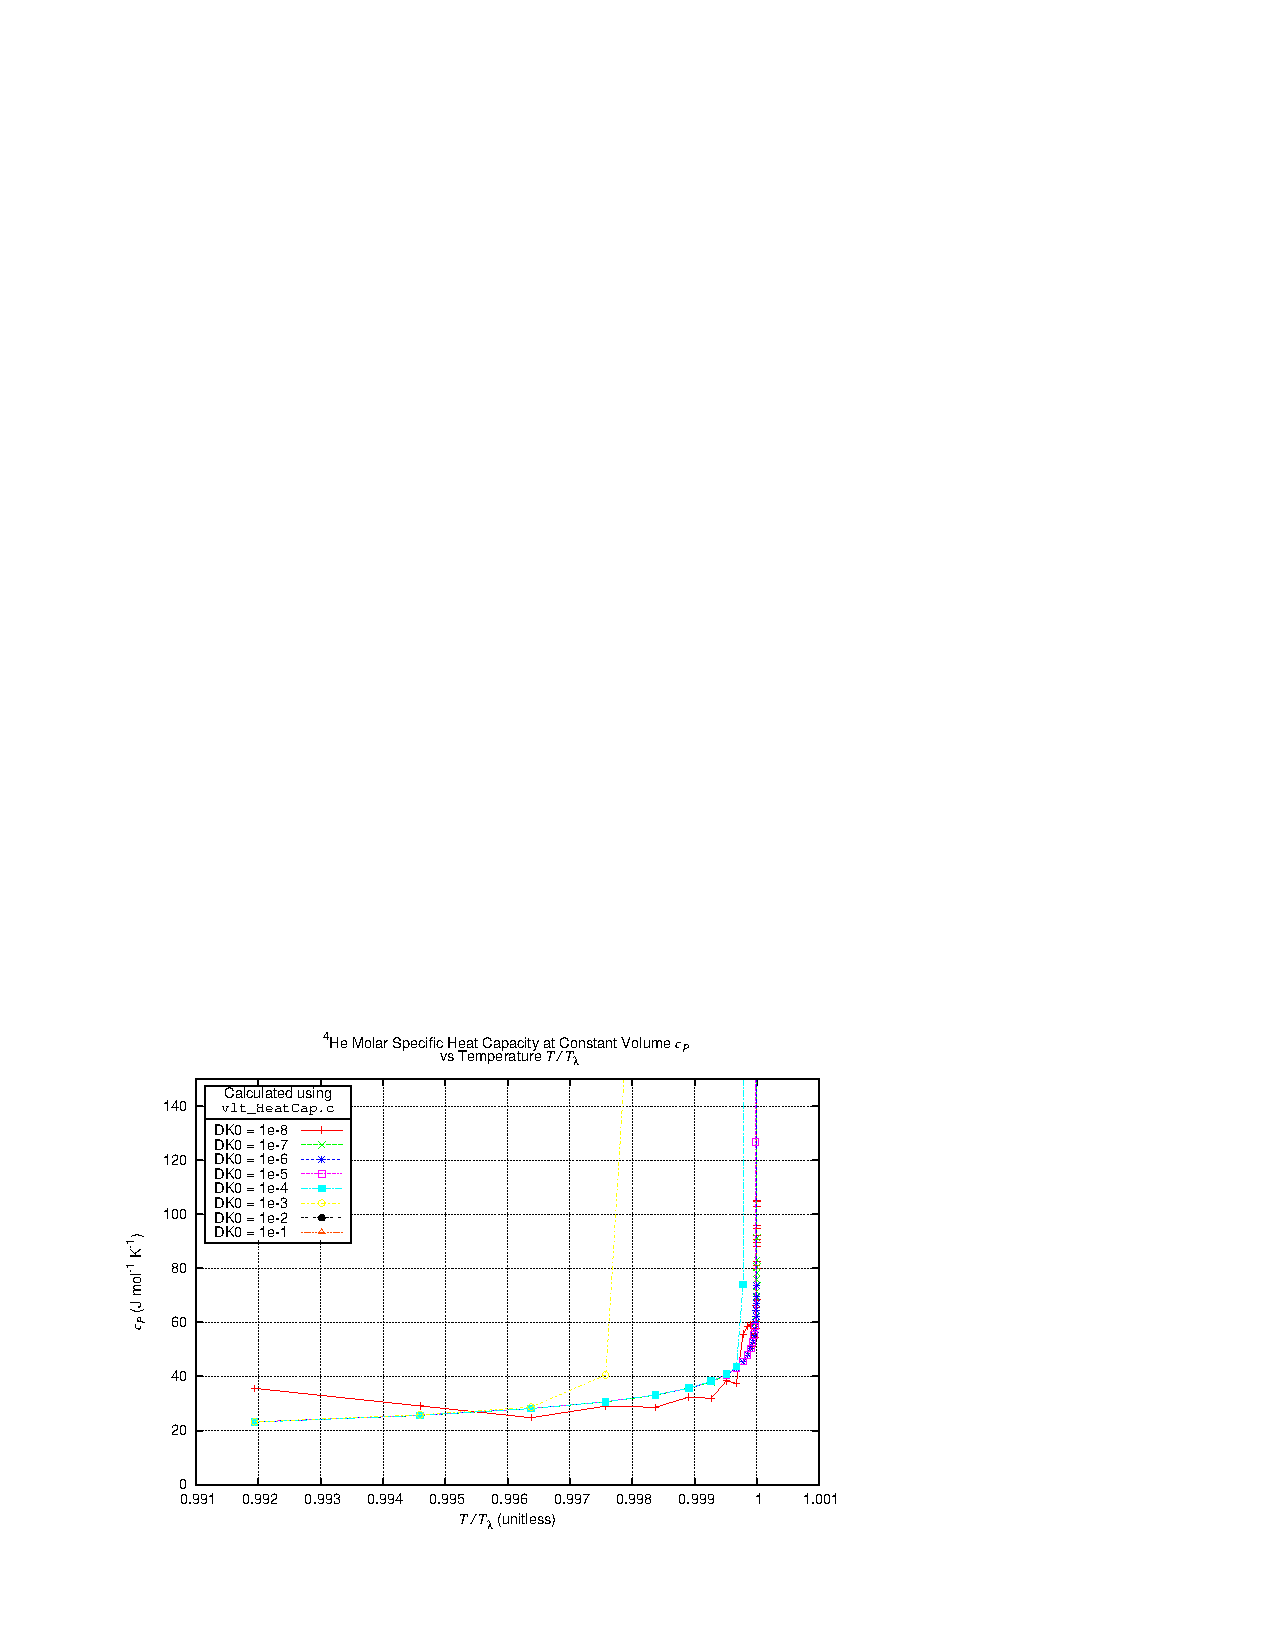
\includegraphics[width=8.5cm,viewport=54 53 410 300]{plot_HeatCapVsTemp.pdf}\newline
  \verb|plot_HeatCapVsTemp.pdf|
\else
  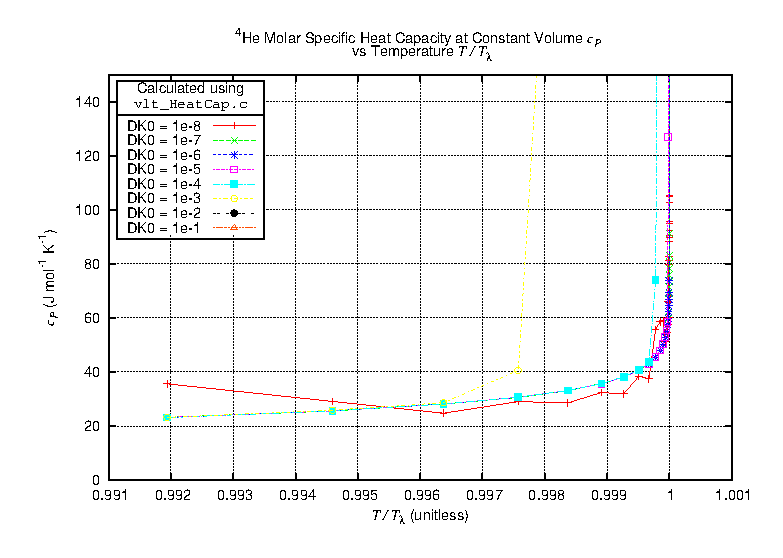
\includegraphics[width=8.5cm]{plot_HeatCapVsTemp.ps}\newline
  \verb|plot_HeatCapVsTemp.ps|
\fi
&
\ifpdf
  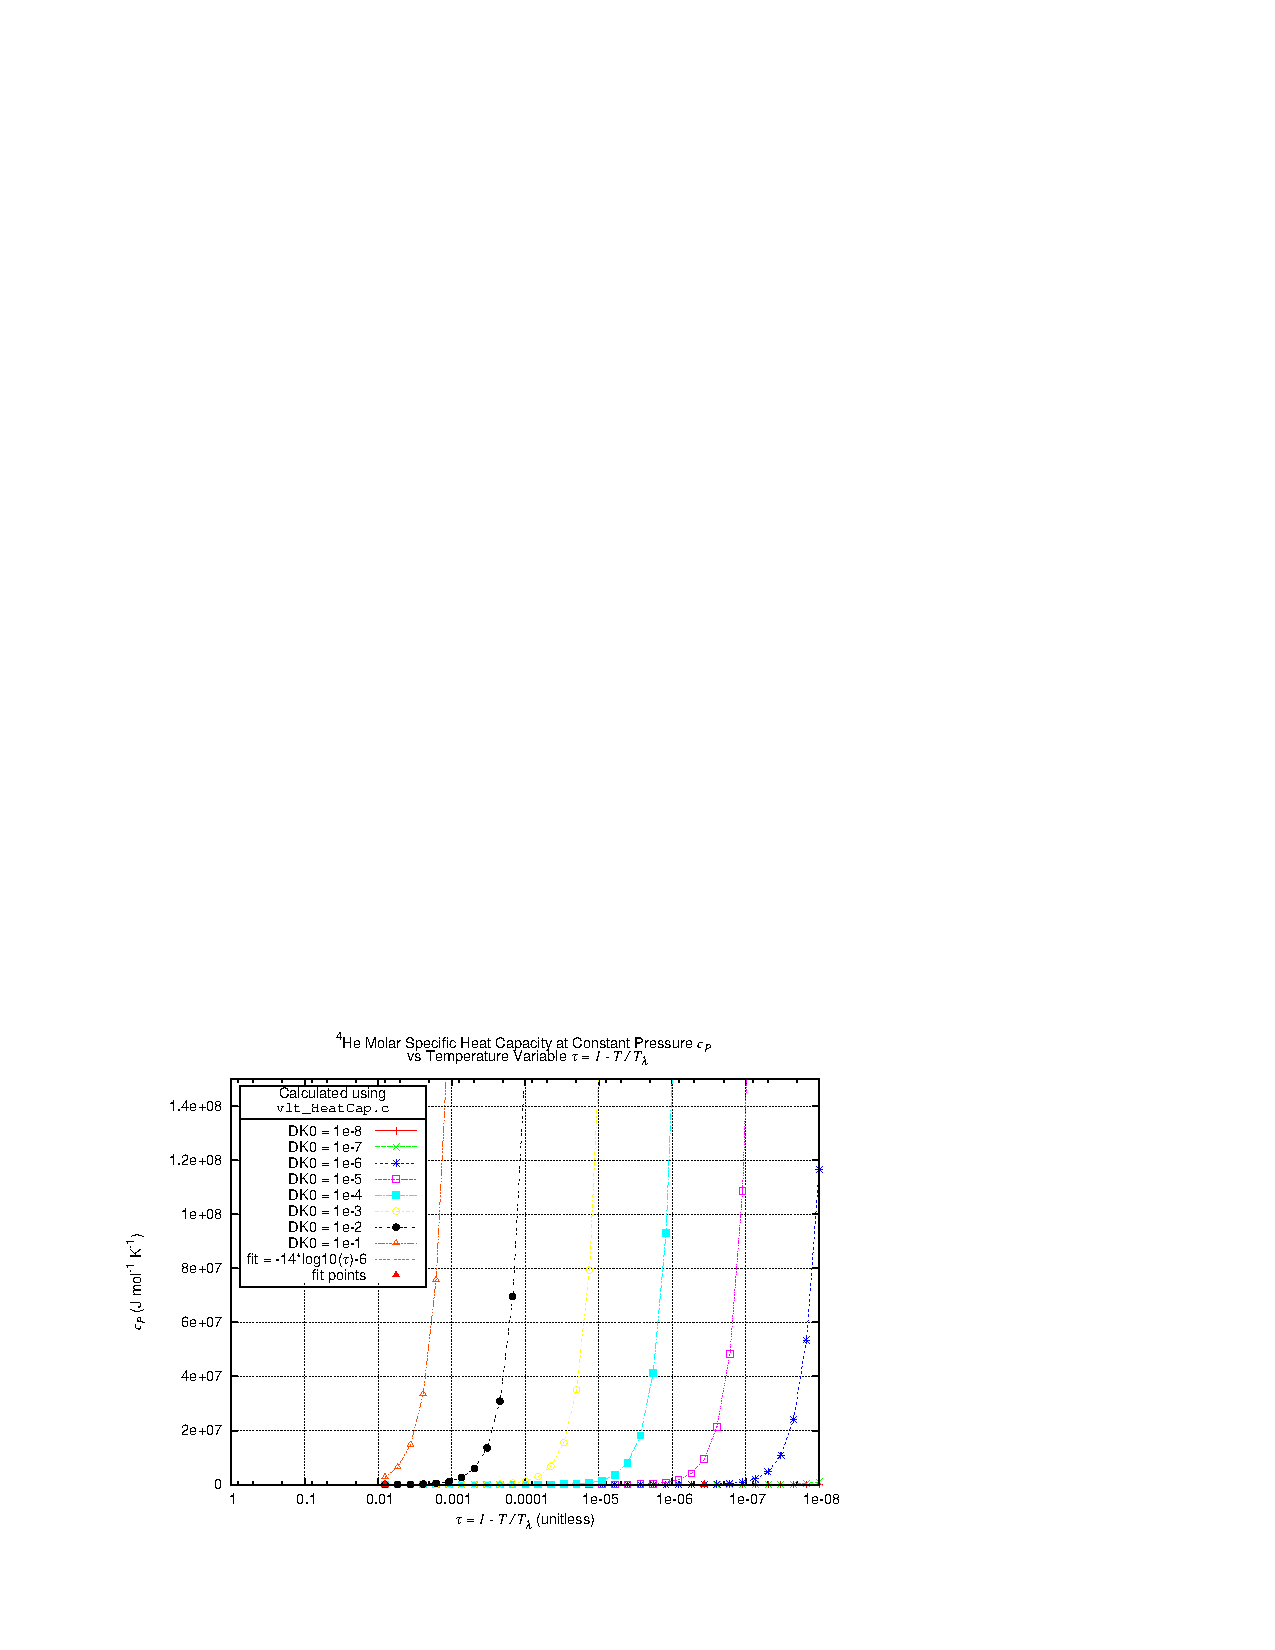
\includegraphics[width=8.5cm,viewport=54 53 410 300]{plot_HeatCapVsTempV_b.pdf}\newline
  \verb|plot_HeatCapVsTempV_b.pdf|
\else
  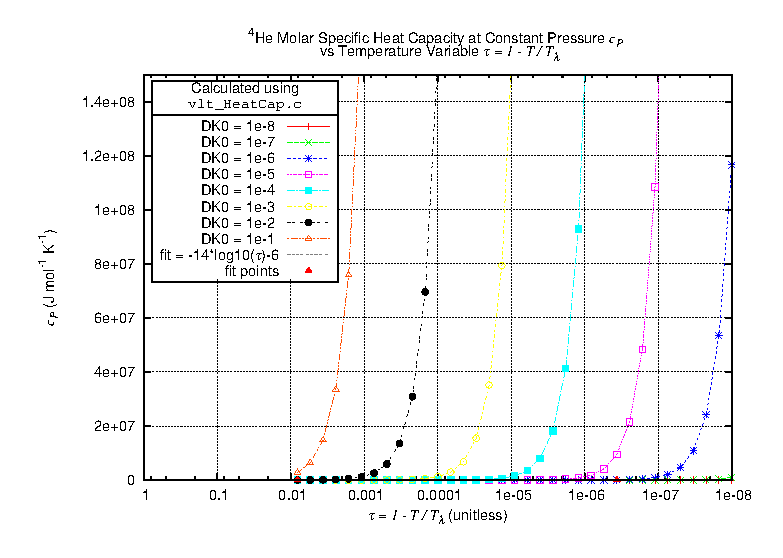
\includegraphics[width=8.5cm]{plot_HeatCapVsTempV_b.ps}\newline
  \verb|plot_HeatCapVsTempV_b.ps|
\fi
 \\
\end{tabular}


The following files are redundant with the three above plots and so are not included (but can be shown if uncommented in \verb|ProgramPlots1.tex| file):
\squishlist
  \item \verb|plot_HeatCapVsTempV_DK0030.ps|
  \item \verb|plot_HeatCapVsTempV_DK0040.ps|
  \item \verb|plot_HeatCapVsTempV_DK0050.ps|
  \item \verb|plot_HeatCapVsTemp_DK0050.ps|
  \item \verb|plot_HeatCapVsTempV_DK0060.ps|
  \item \verb|plot_HeatCapVsTempV_DK0070.ps|
  \item \verb|plot_HeatCapVsTempV_DK0080.ps|
  \item \verb|plot_HeatCapVsTempV_DK0090.ps|
  \item \verb|plot_HeatCapVsTempV_DK0100.ps|
  \item \verb|plot_HeatCapVsTempV_DK0110.ps|
  \item \verb|plot_HeatCapVsTempV_DK0120.ps|
  \item \verb|plot_HeatCapVsTempV_DK0130.ps|
  \item \verb|plot_HeatCapVsTempV_DK0140.ps|
  \item \verb|plot_HeatCapVsTvPress.ps|
\squishend



\begin{comment}

\begin{center}
\begin{tabular}[\textwidth]{p{8.5cm}p{8.5cm}}
\ifpdf
  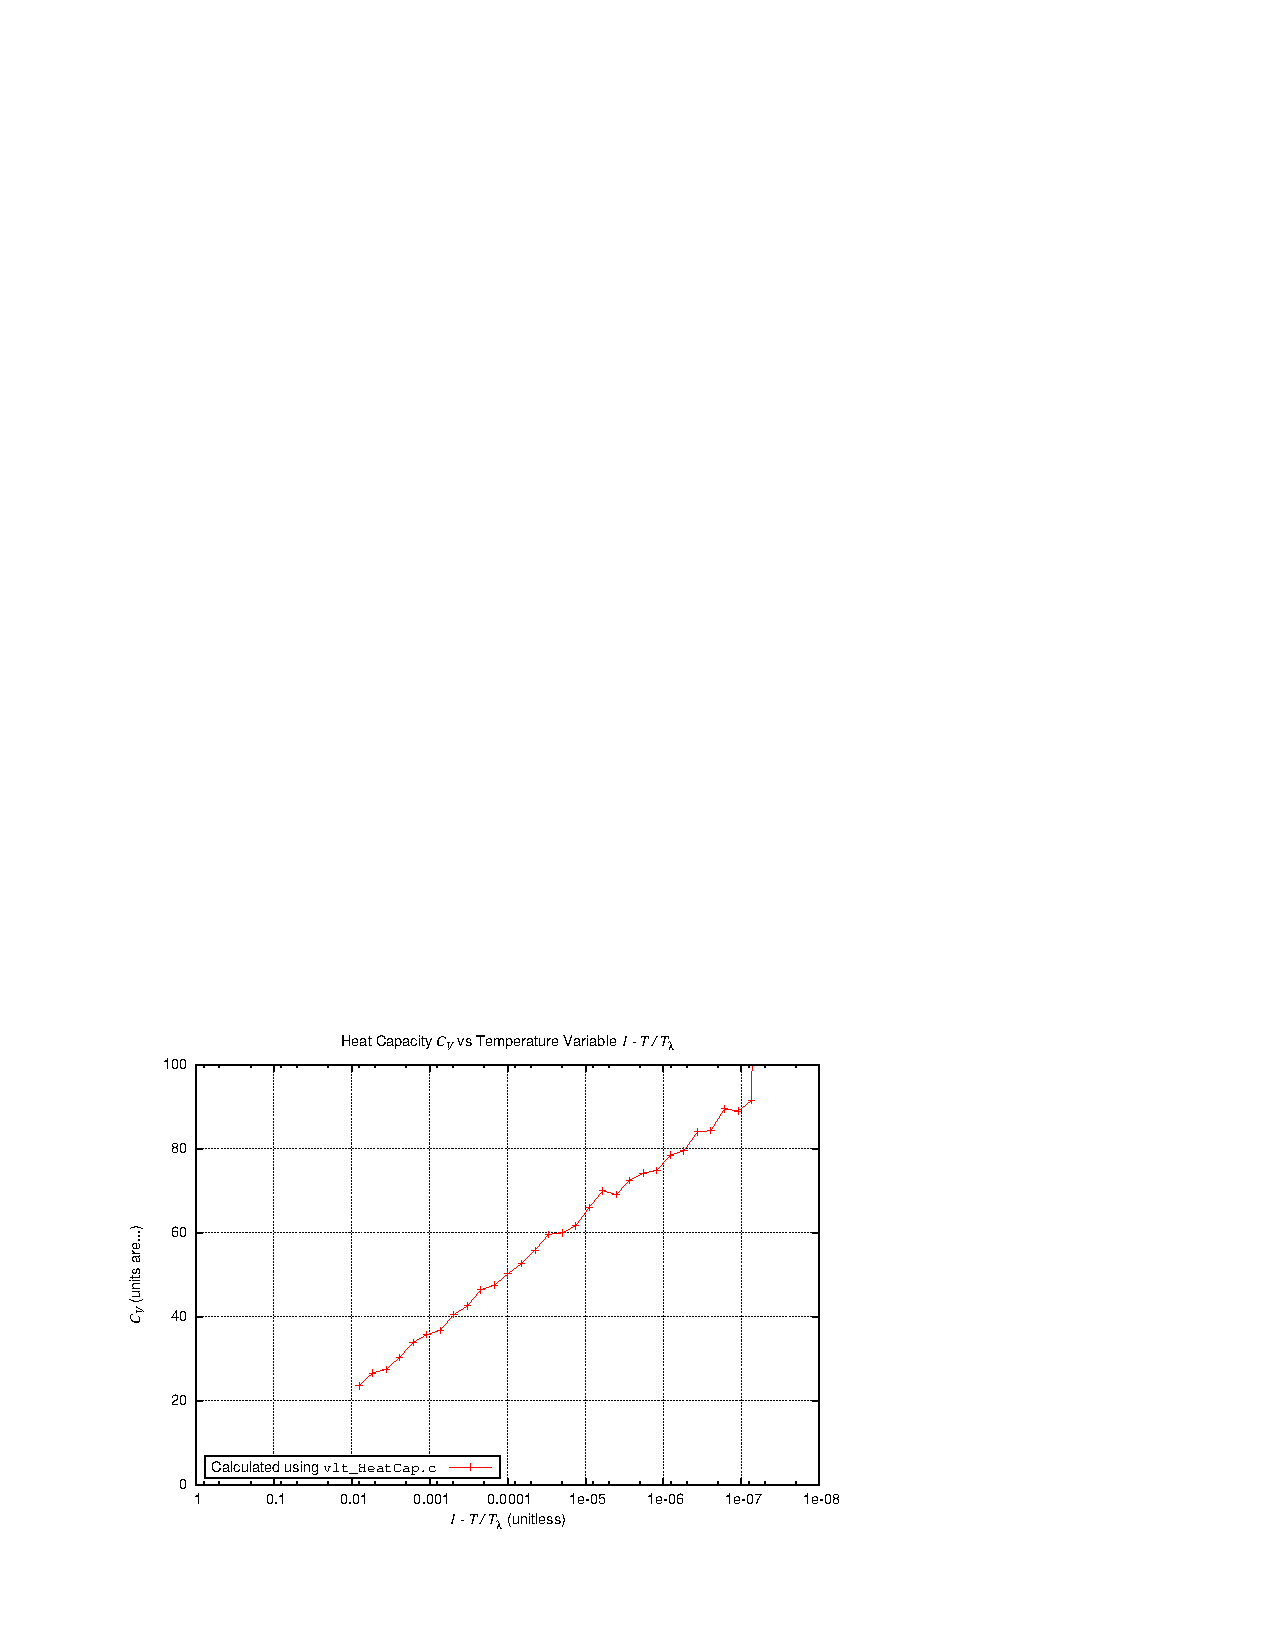
\includegraphics[width=8.5cm,viewport=54 53 410 300]{plot_HeatCapVsTempV_DK0030.pdf}\newline
  \verb|plot_HeatCapVsTempV_DK0030.pdf|
\else
  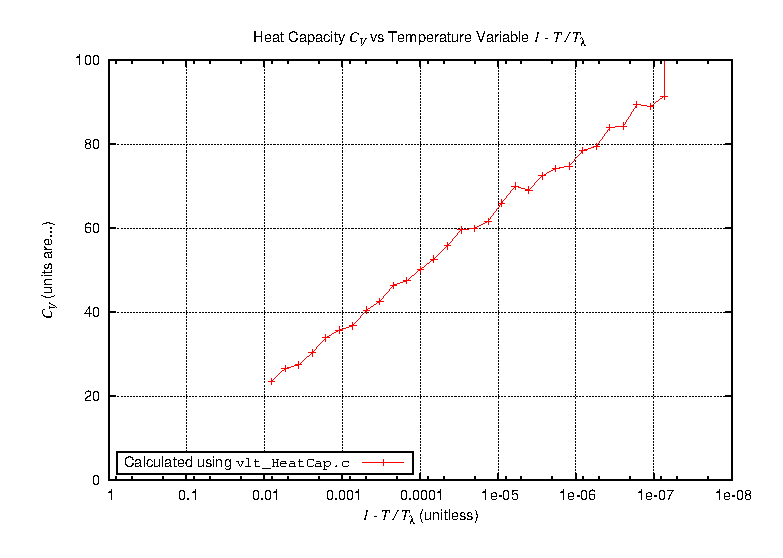
\includegraphics[width=8.5cm]{plot_HeatCapVsTempV_DK0030.ps}\newline
  \verb|plot_HeatCapVsTempV_DK0030.ps|
\fi
&
\ifpdf
  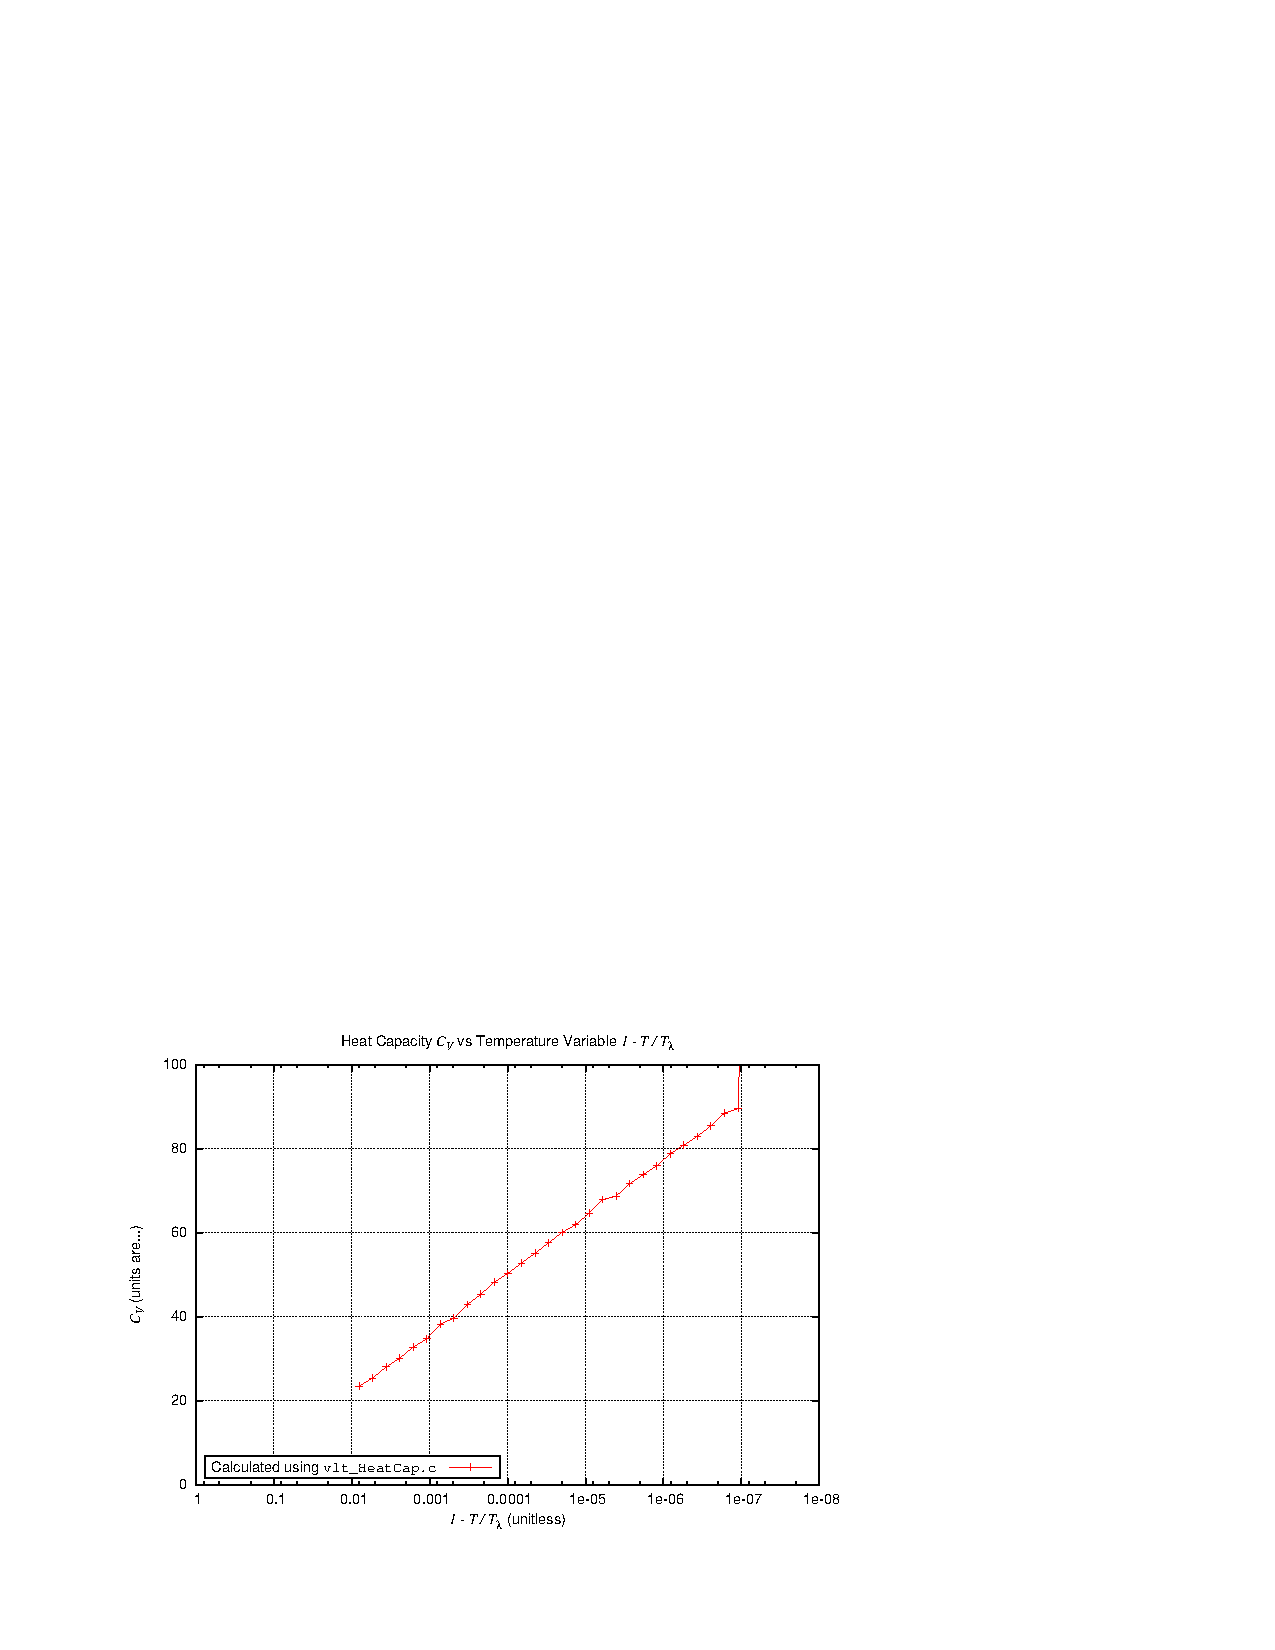
\includegraphics[width=8.5cm,viewport=54 53 410 300]{plot_HeatCapVsTempV_DK0040.pdf}\newline
  \verb|plot_HeatCapVsTempV_DK0040.pdf|
\else
  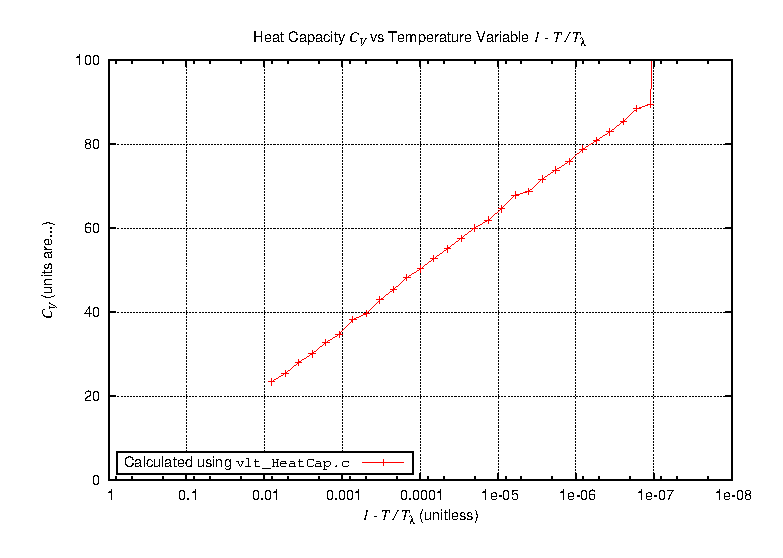
\includegraphics[width=8.5cm]{plot_HeatCapVsTempV_DK0040.ps}\newline
  \verb|plot_HeatCapVsTempV_DK0040.ps|
\fi
 \\
\ifpdf
  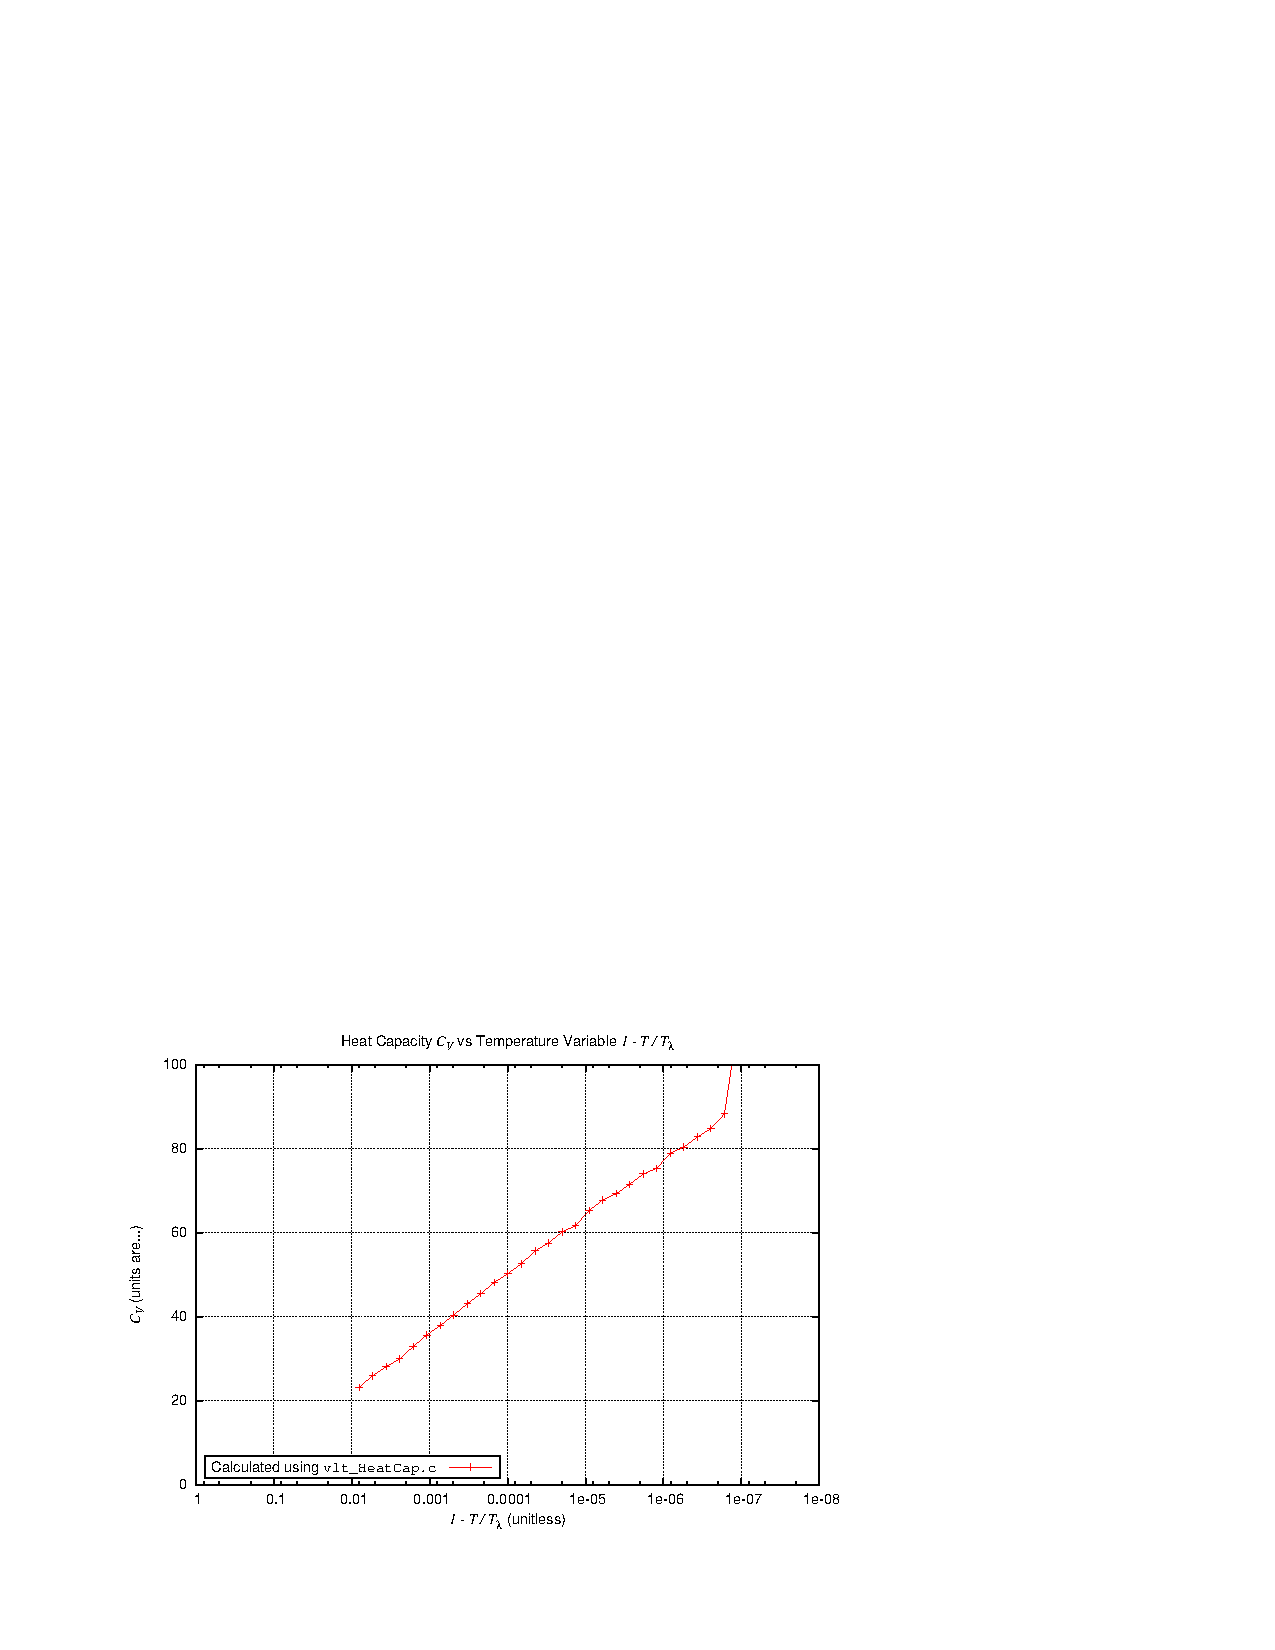
\includegraphics[width=8.5cm,viewport=54 53 410 300]{plot_HeatCapVsTempV_DK0050.pdf}\newline
  \verb|plot_HeatCapVsTempV_DK0050.pdf|
\else
  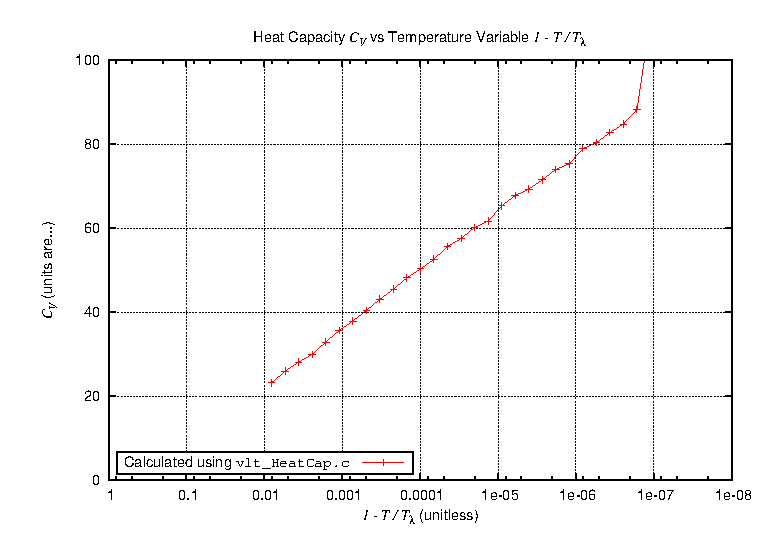
\includegraphics[width=8.5cm]{plot_HeatCapVsTempV_DK0050.ps}\newline
  \verb|plot_HeatCapVsTempV_DK0050.ps|
\fi
&
\ifpdf
  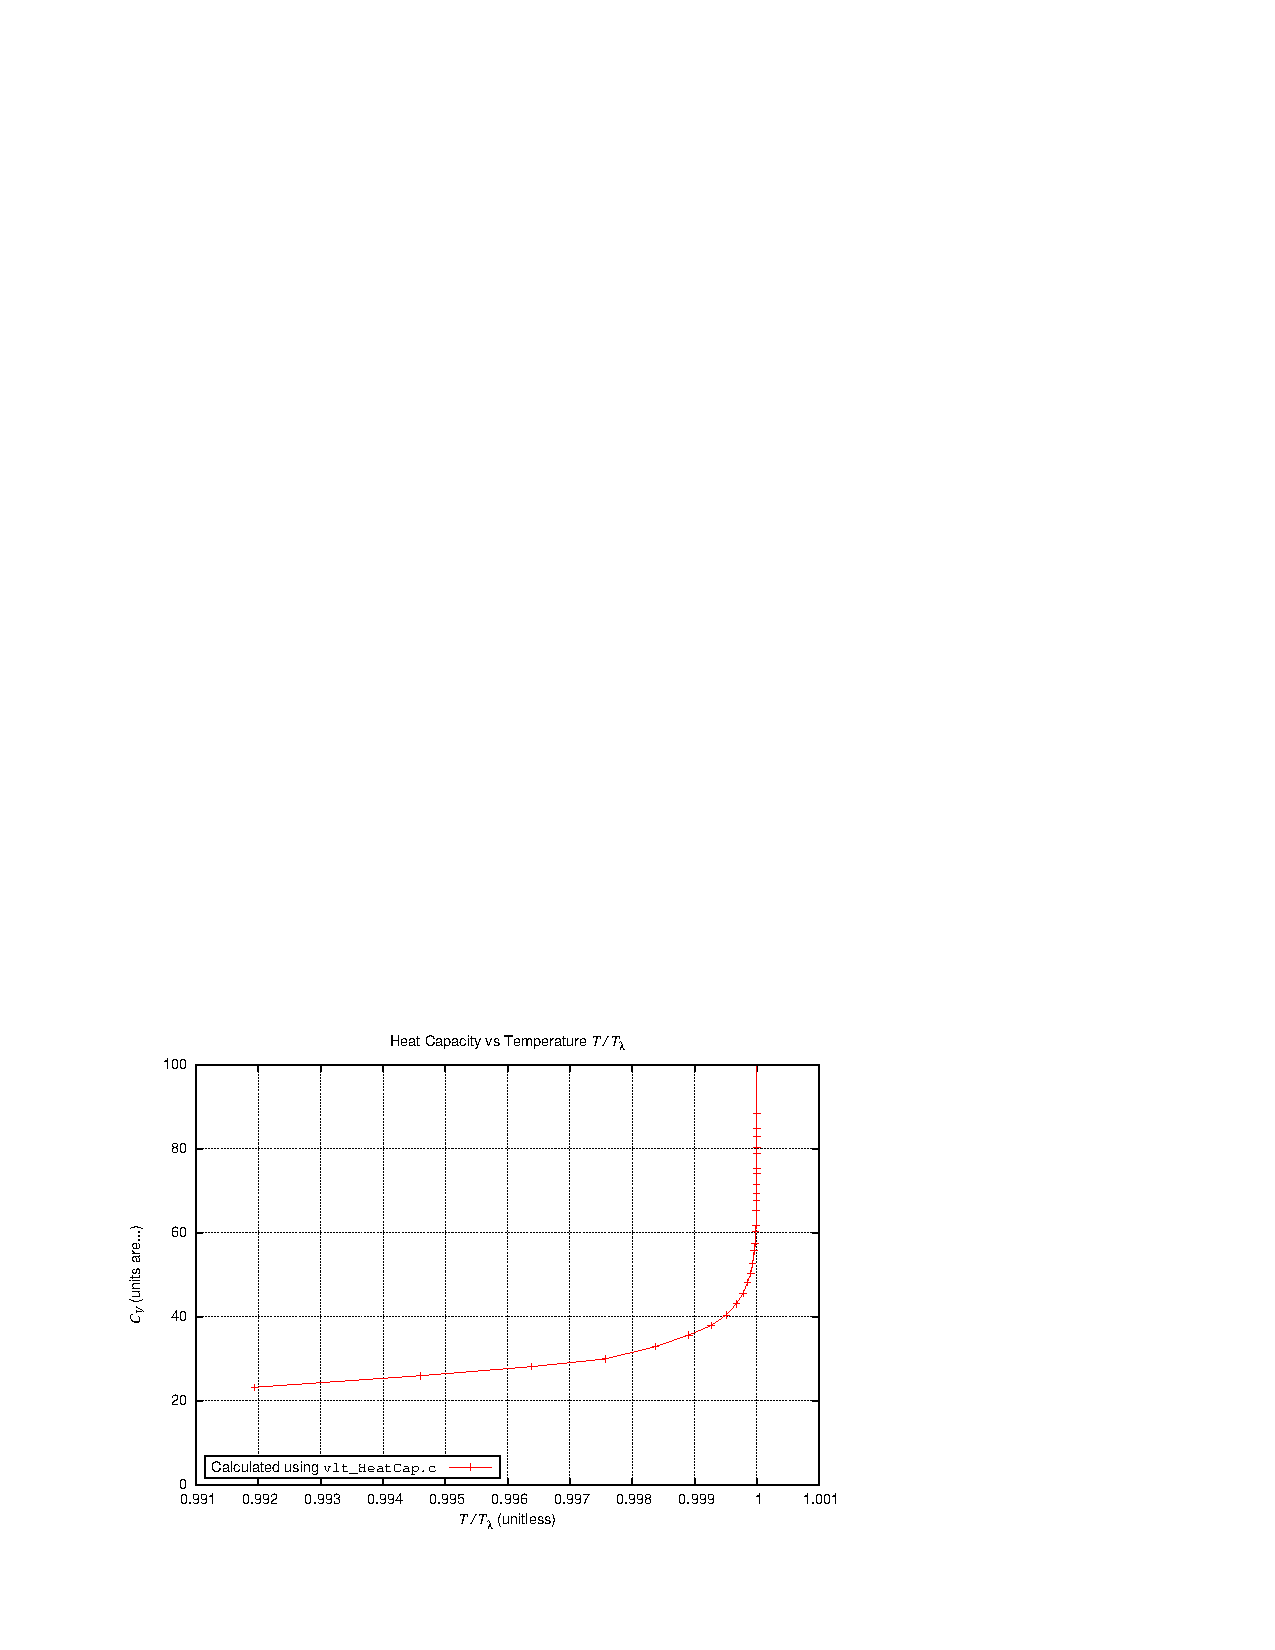
\includegraphics[width=8.5cm,viewport=54 53 410 300]{plot_HeatCapVsTemp_DK0050.pdf}\newline
  \verb|plot_HeatCapVsTemp_DK0050.pdf|
\else
  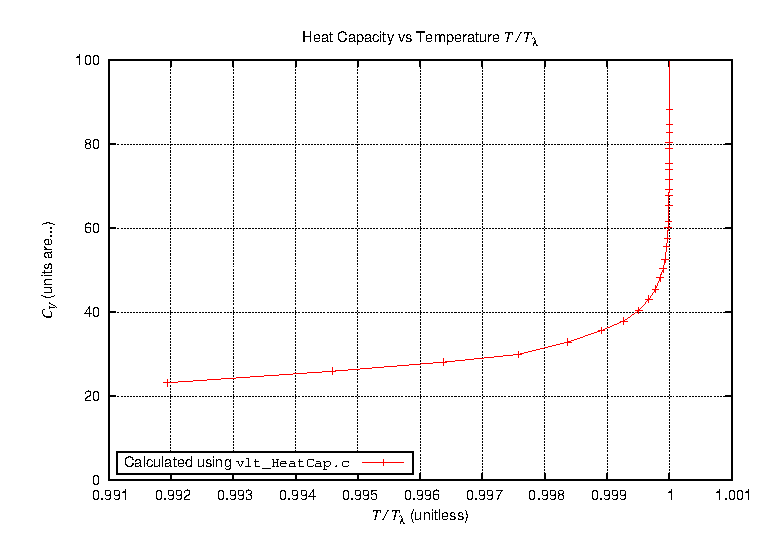
\includegraphics[width=8.5cm]{plot_HeatCapVsTemp_DK0050.ps}\newline
  \verb|plot_HeatCapVsTemp_DK0050.ps|
\fi
 \\
\ifpdf
  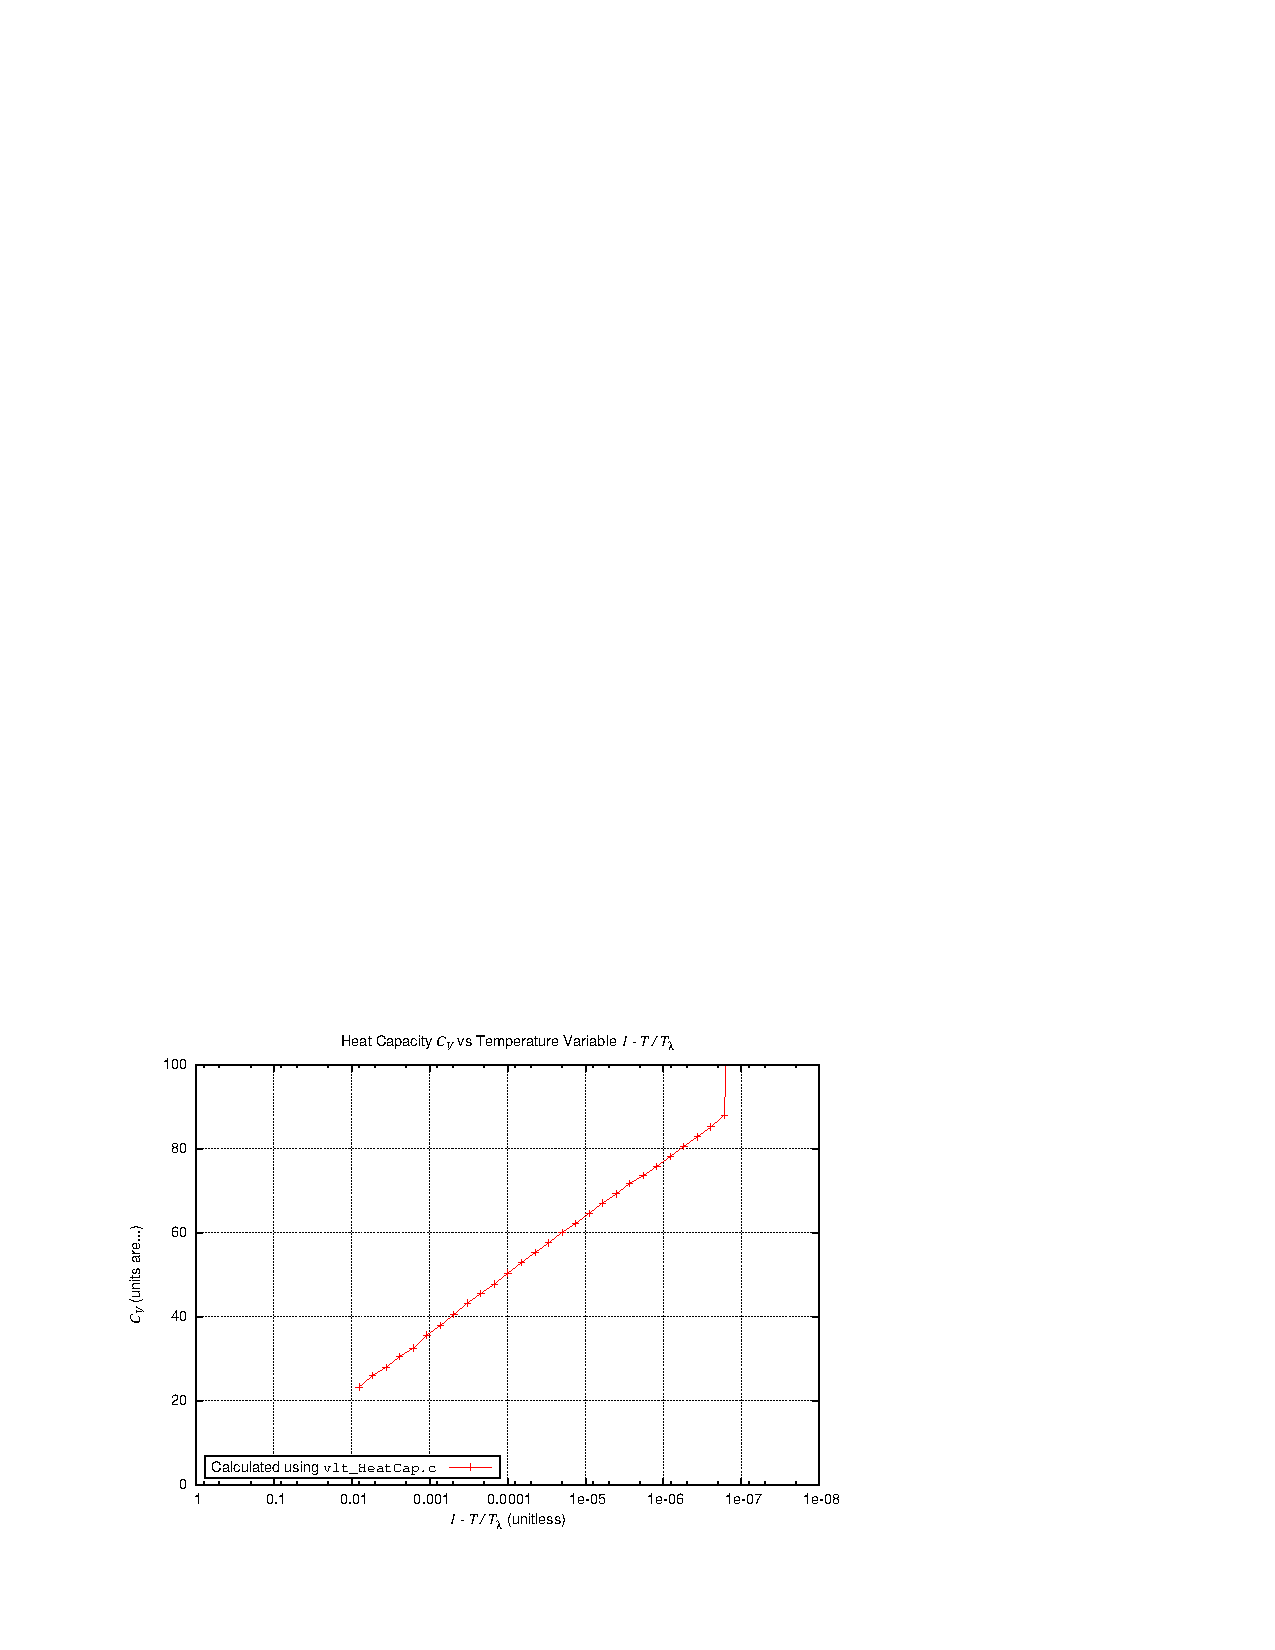
\includegraphics[width=8.5cm,viewport=54 53 410 300]{plot_HeatCapVsTempV_DK0060.pdf}\newline
  \verb|plot_HeatCapVsTempV_DK0060.pdf|
\else
  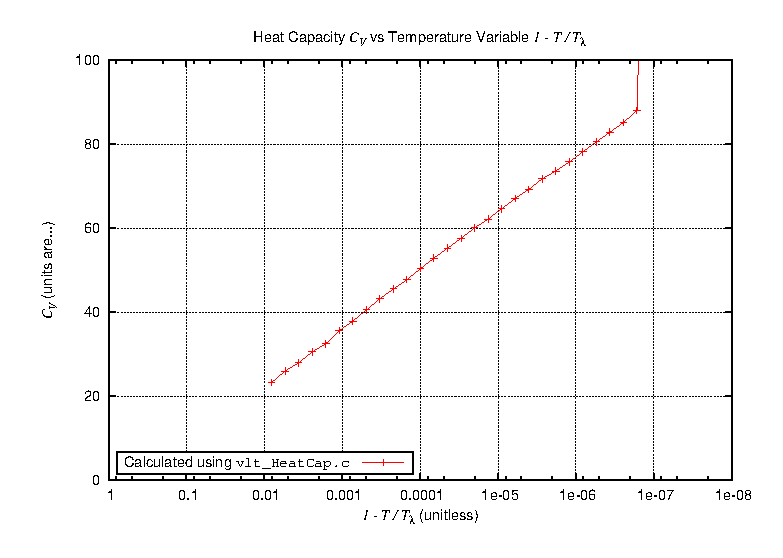
\includegraphics[width=8.5cm]{plot_HeatCapVsTempV_DK0060.ps}\newline
  \verb|plot_HeatCapVsTempV_DK0060.ps|
\fi
&
\ifpdf
  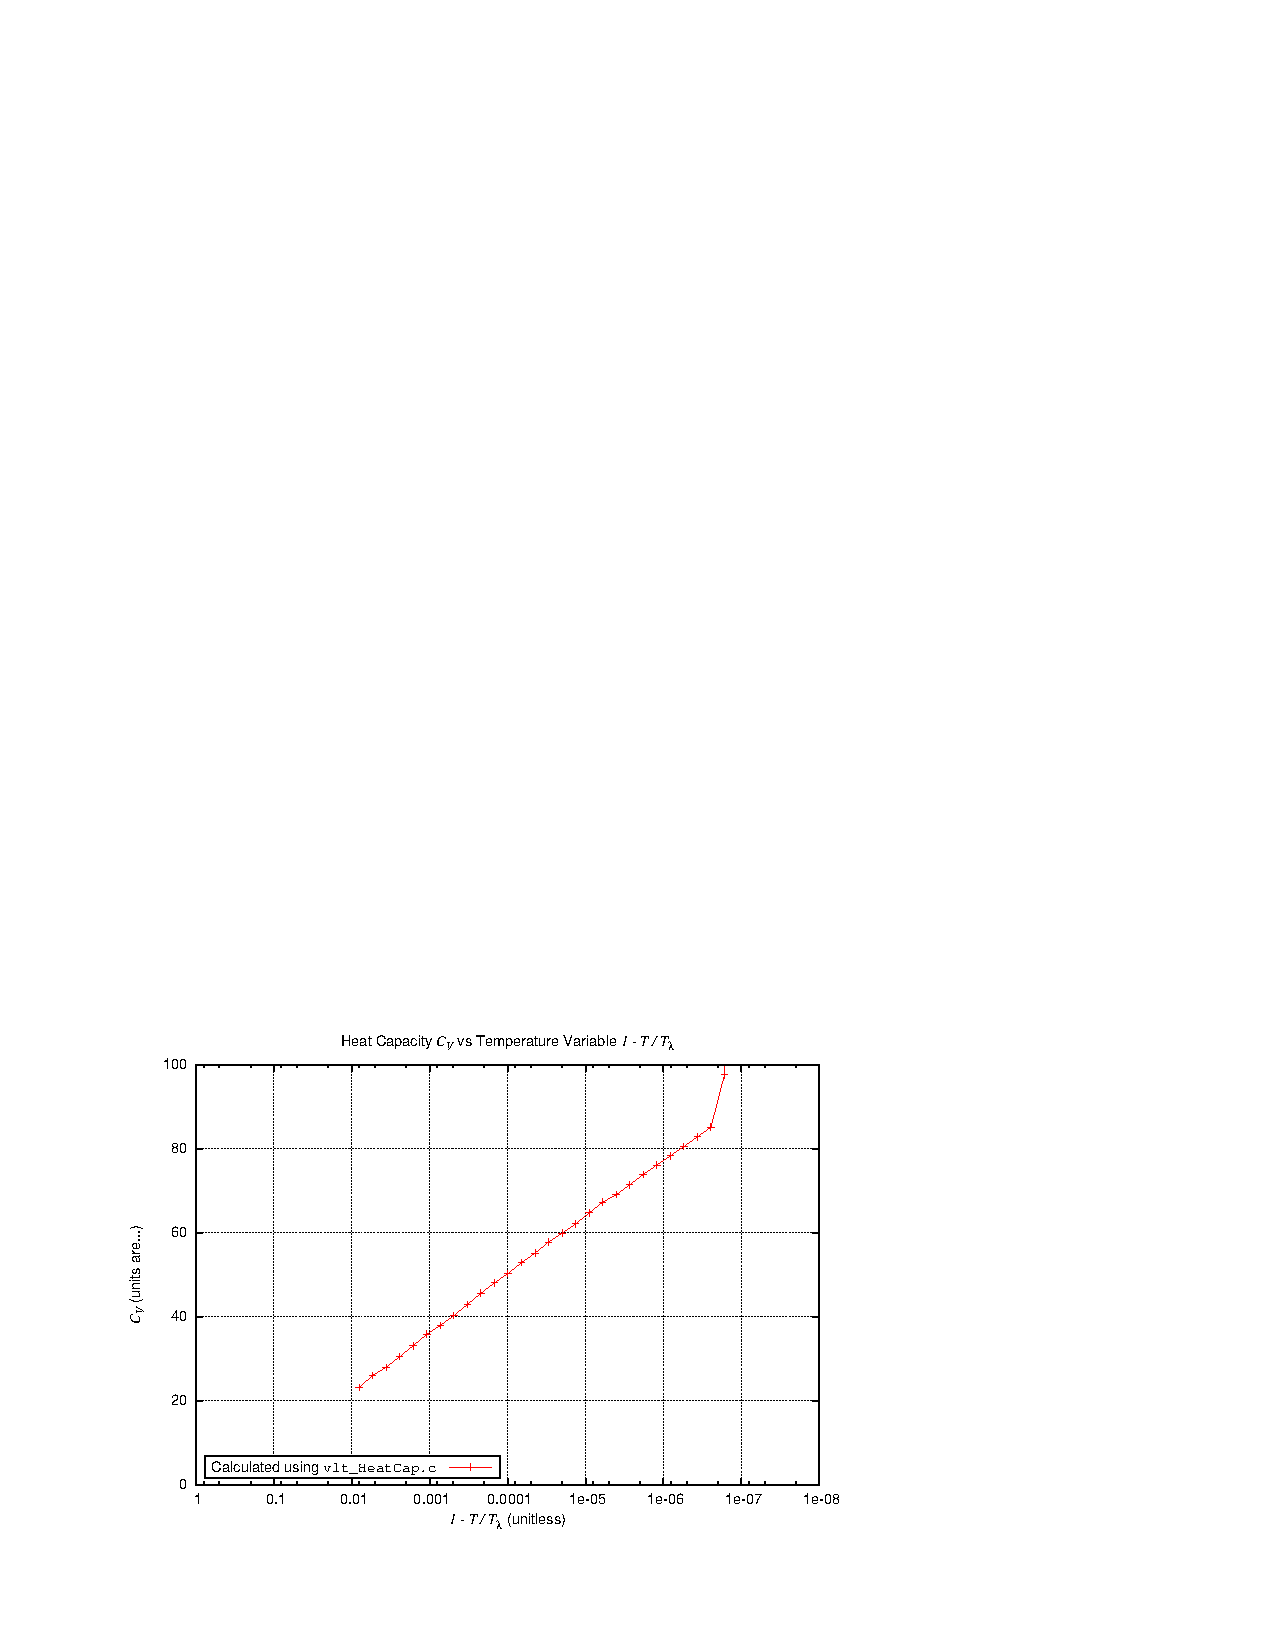
\includegraphics[width=8.5cm,viewport=54 53 410 300]{plot_HeatCapVsTempV_DK0070.pdf}\newline
  \verb|plot_HeatCapVsTempV_DK0070.pdf|
\else
  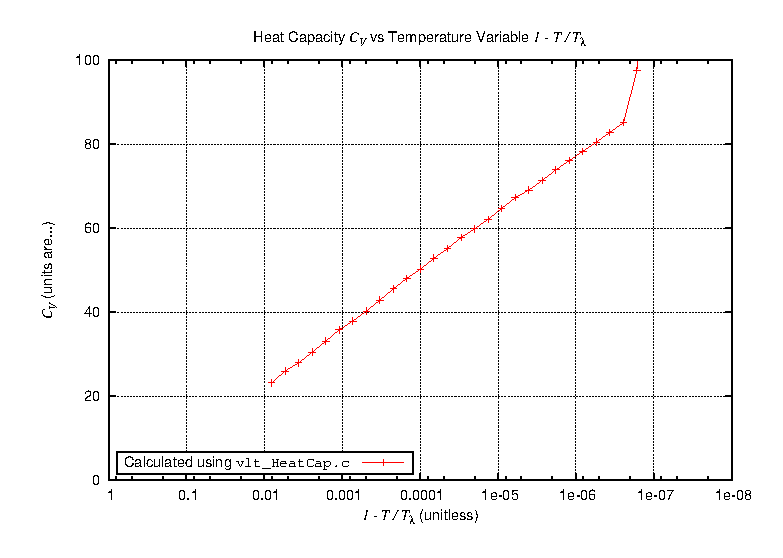
\includegraphics[width=8.5cm]{plot_HeatCapVsTempV_DK0070.ps}\newline
  \verb|plot_HeatCapVsTempV_DK0070.ps|
\fi
 \\
\end{tabular}
\end{center}


\begin{center}
\begin{tabular}[\textwidth]{p{8.5cm}p{8.5cm}}
\ifpdf
  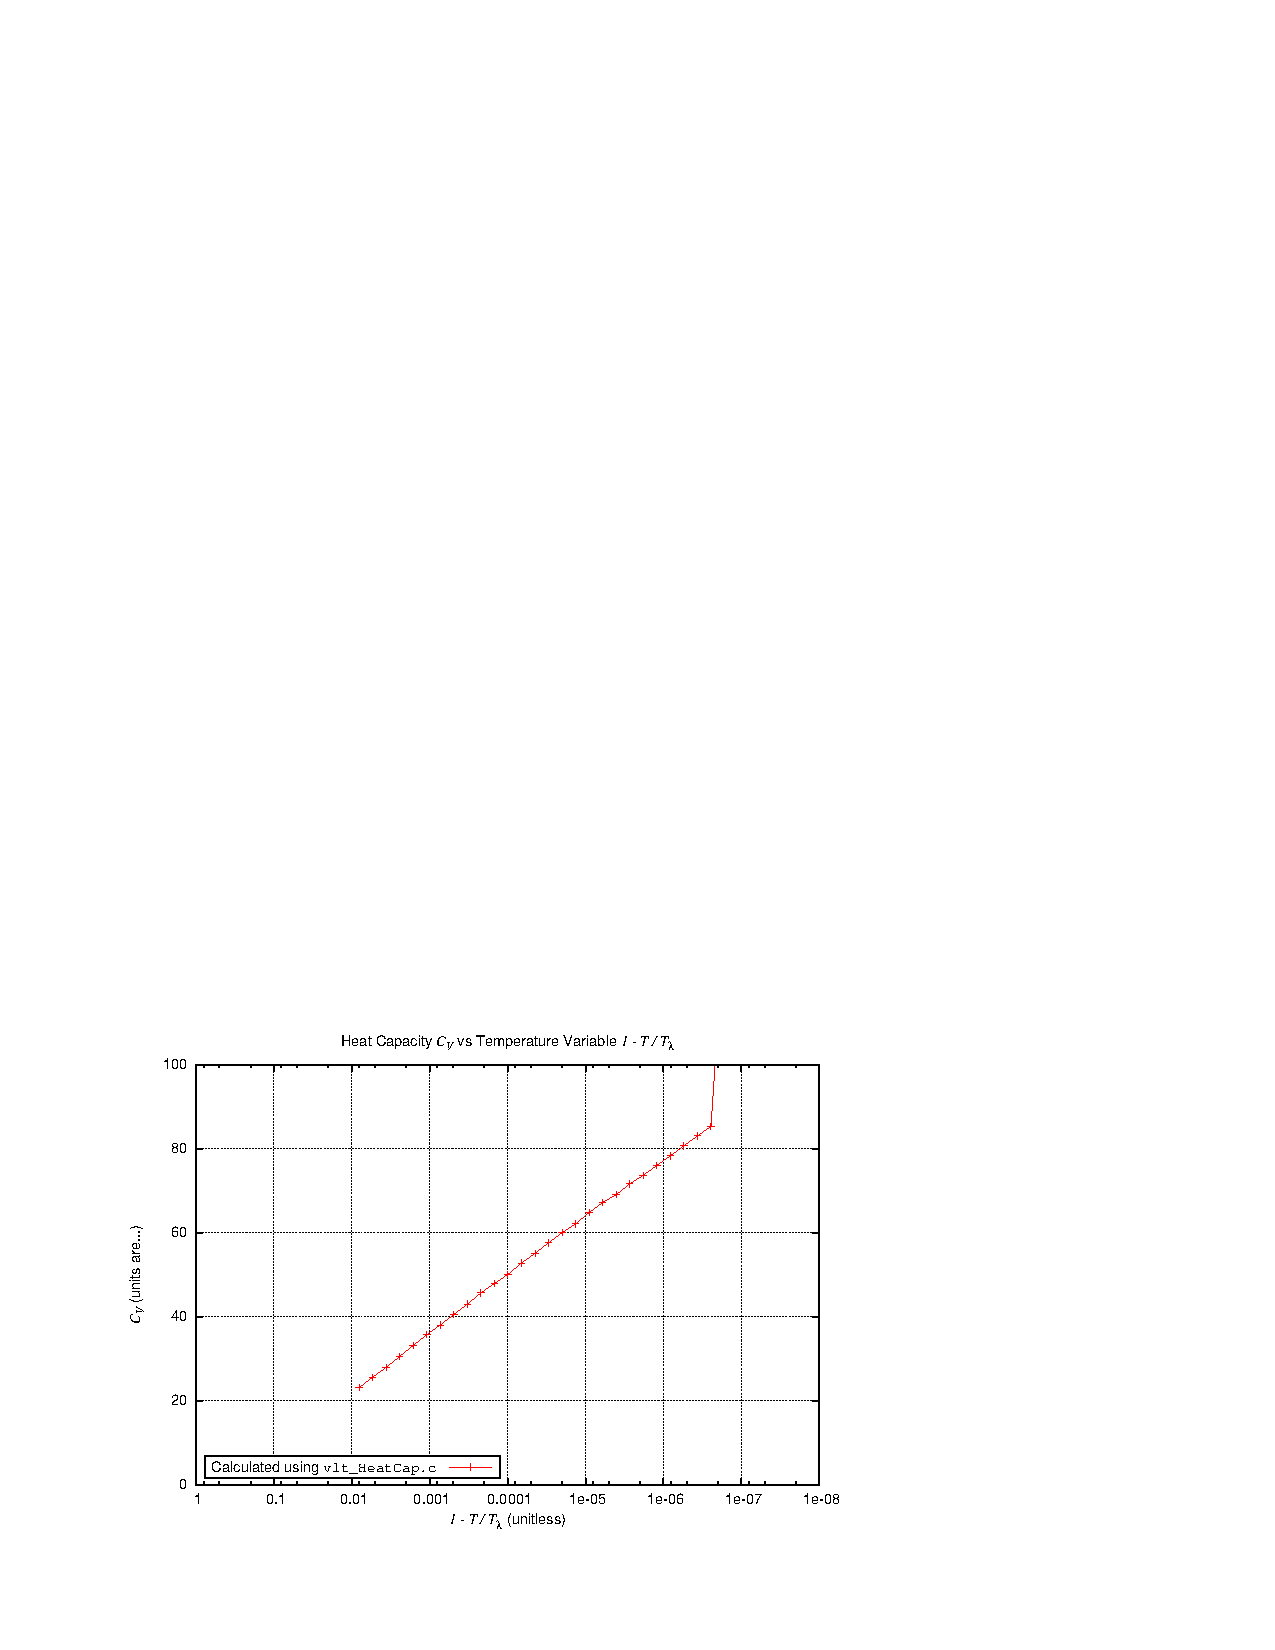
\includegraphics[width=8.5cm,viewport=54 53 410 300]{plot_HeatCapVsTempV_DK0080.pdf}\newline
  \verb|plot_HeatCapVsTempV_DK0080.pdf|
\else
  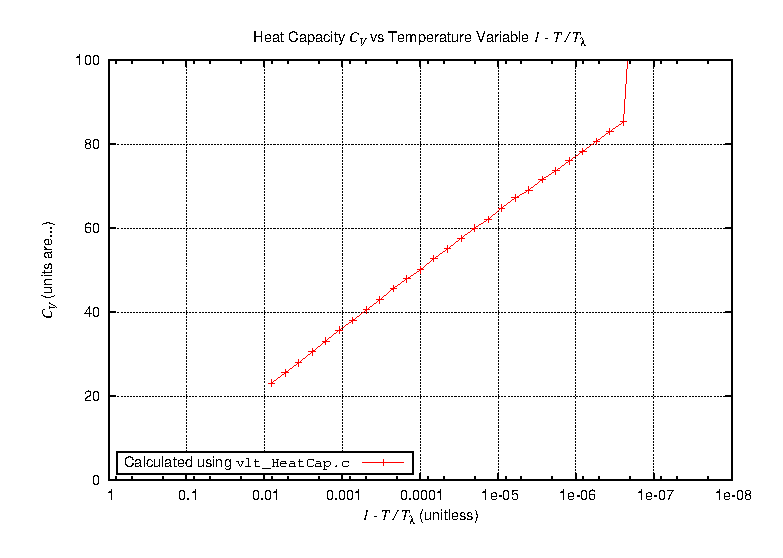
\includegraphics[width=8.5cm]{plot_HeatCapVsTempV_DK0080.ps}\newline
  \verb|plot_HeatCapVsTempV_DK0080.ps|
\fi
&
\ifpdf
  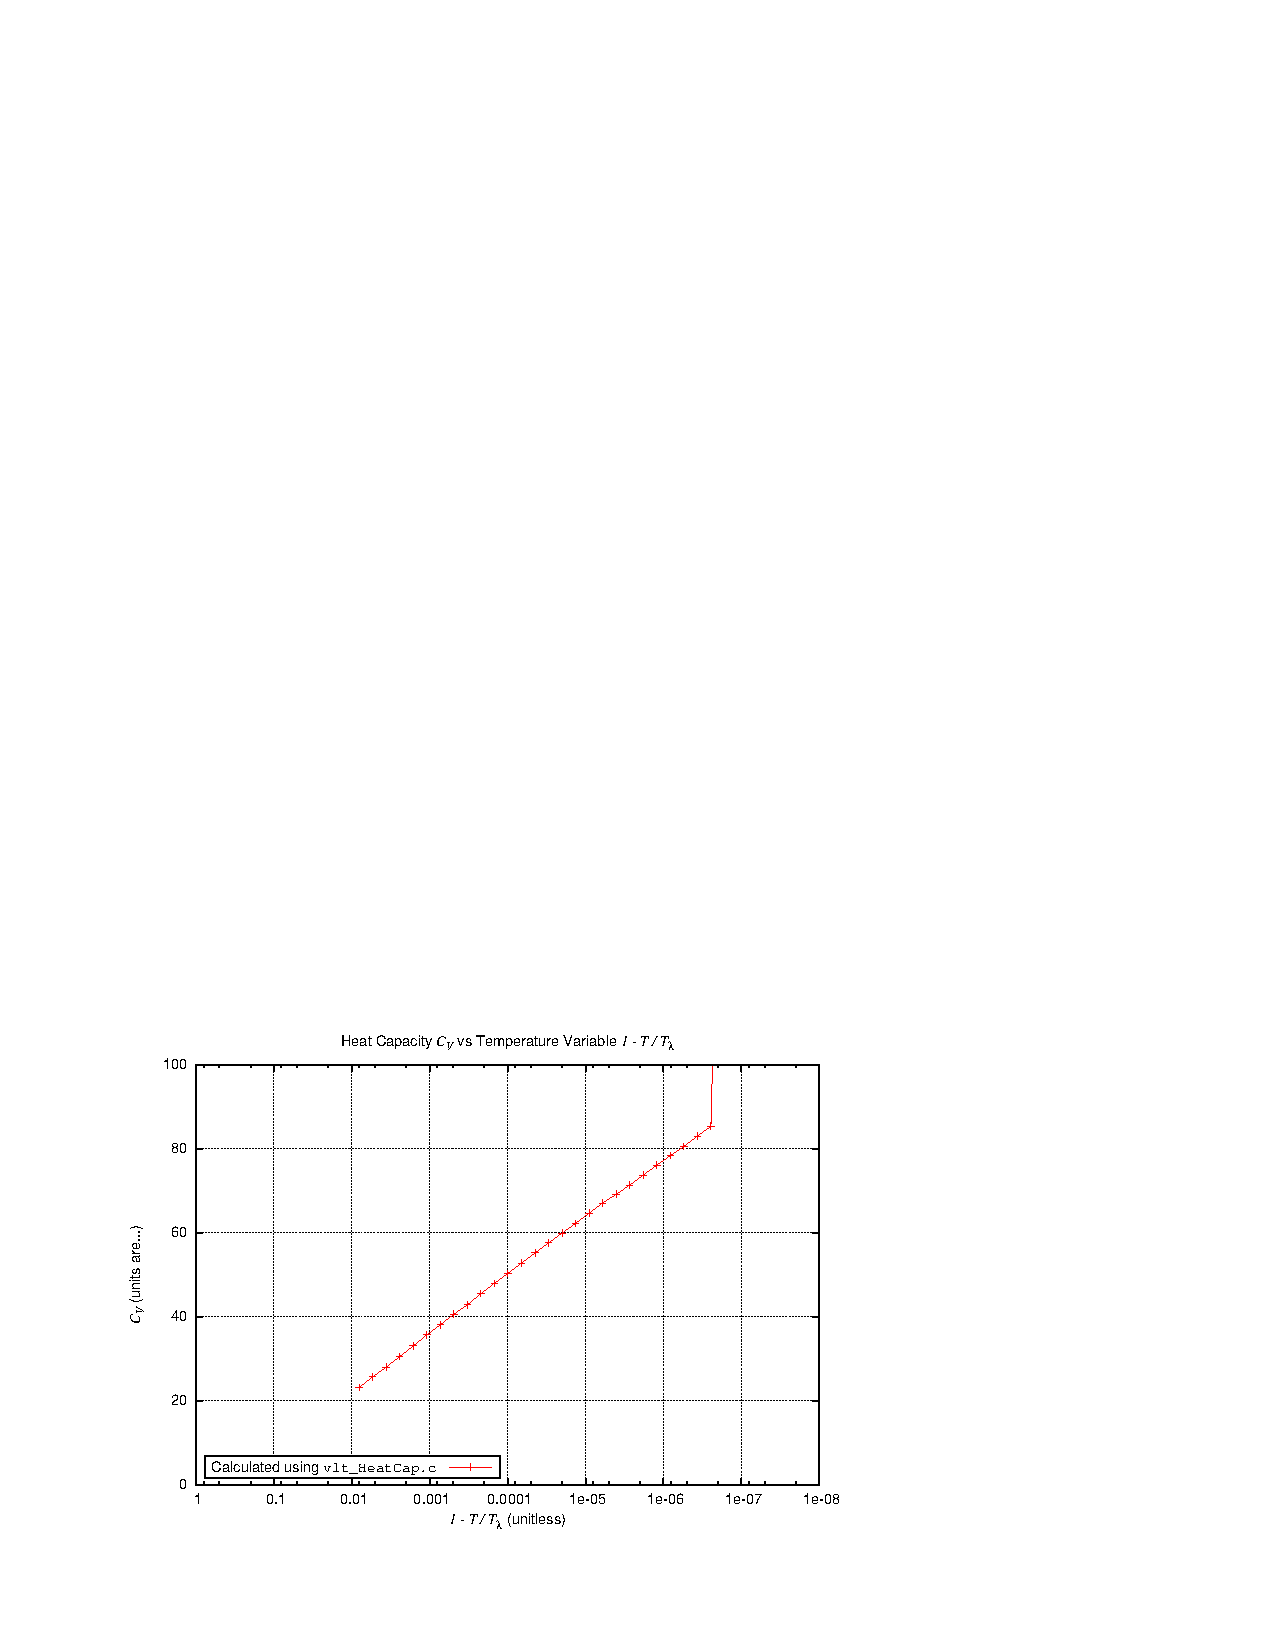
\includegraphics[width=8.5cm,viewport=54 53 410 300]{plot_HeatCapVsTempV_DK0090.pdf}\newline
  \verb|plot_HeatCapVsTempV_DK0090.pdf|
\else
  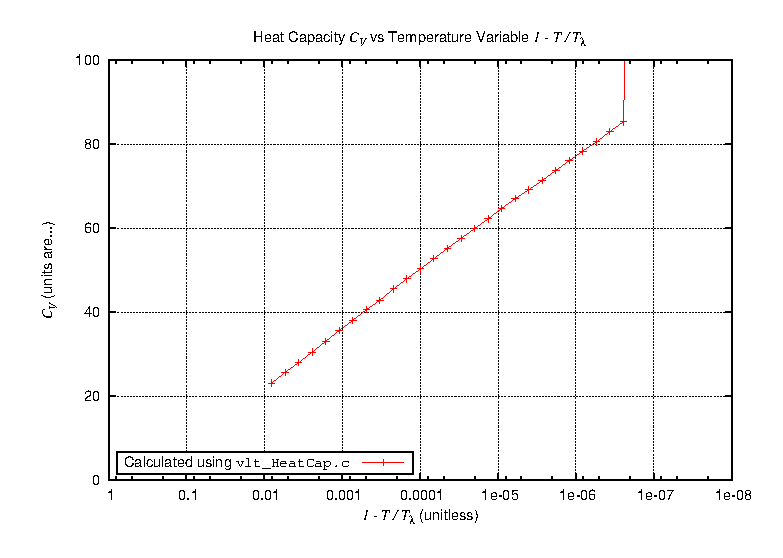
\includegraphics[width=8.5cm]{plot_HeatCapVsTempV_DK0090.ps}\newline
  \verb|plot_HeatCapVsTempV_DK0090.ps|
\fi
 \\
\ifpdf
  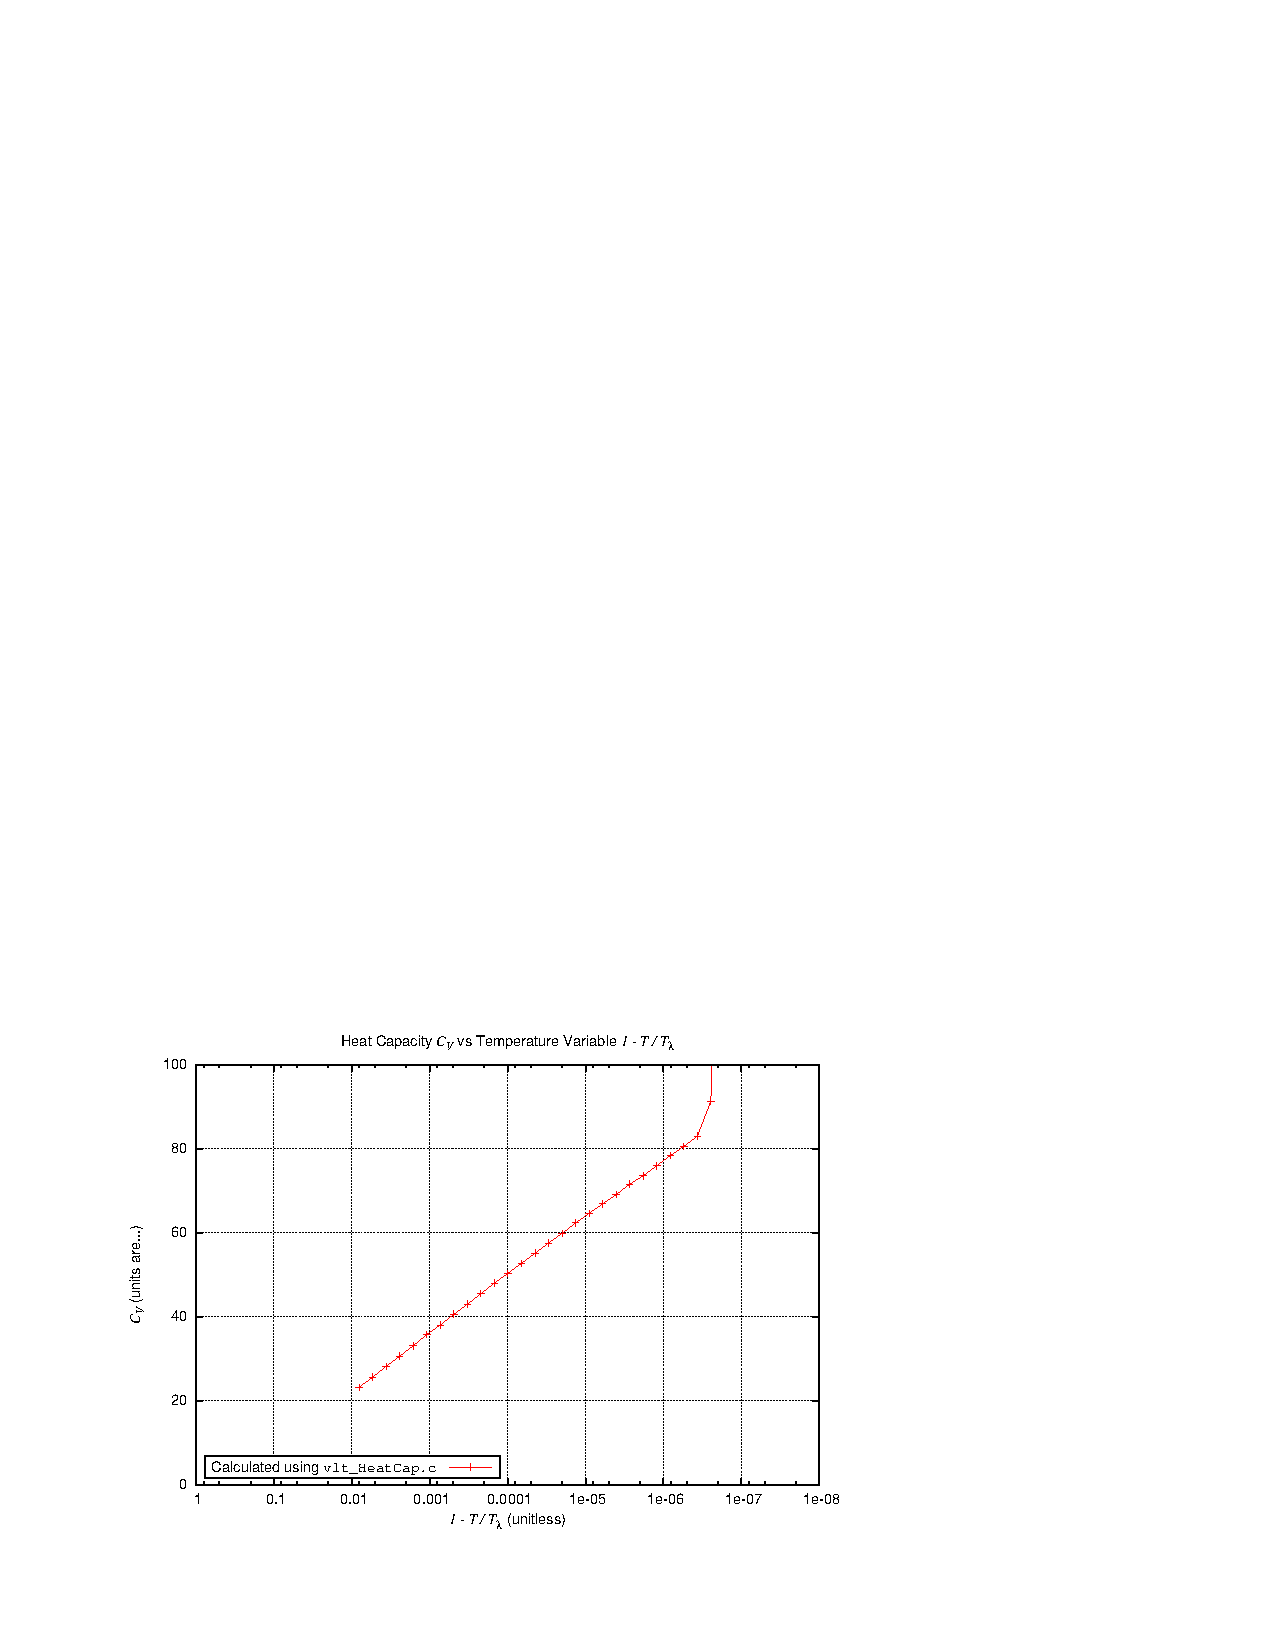
\includegraphics[width=8.5cm,viewport=54 53 410 300]{plot_HeatCapVsTempV_DK0100.pdf}\newline
  \verb|plot_HeatCapVsTempV_DK0100.pdf|
\else
  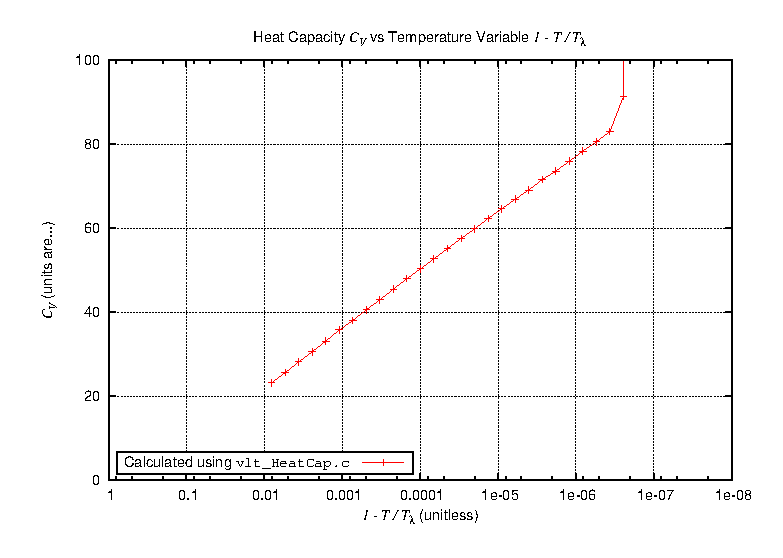
\includegraphics[width=8.5cm]{plot_HeatCapVsTempV_DK0100.ps}\newline
  \verb|plot_HeatCapVsTempV_DK0100.ps|
\fi
&
\ifpdf
  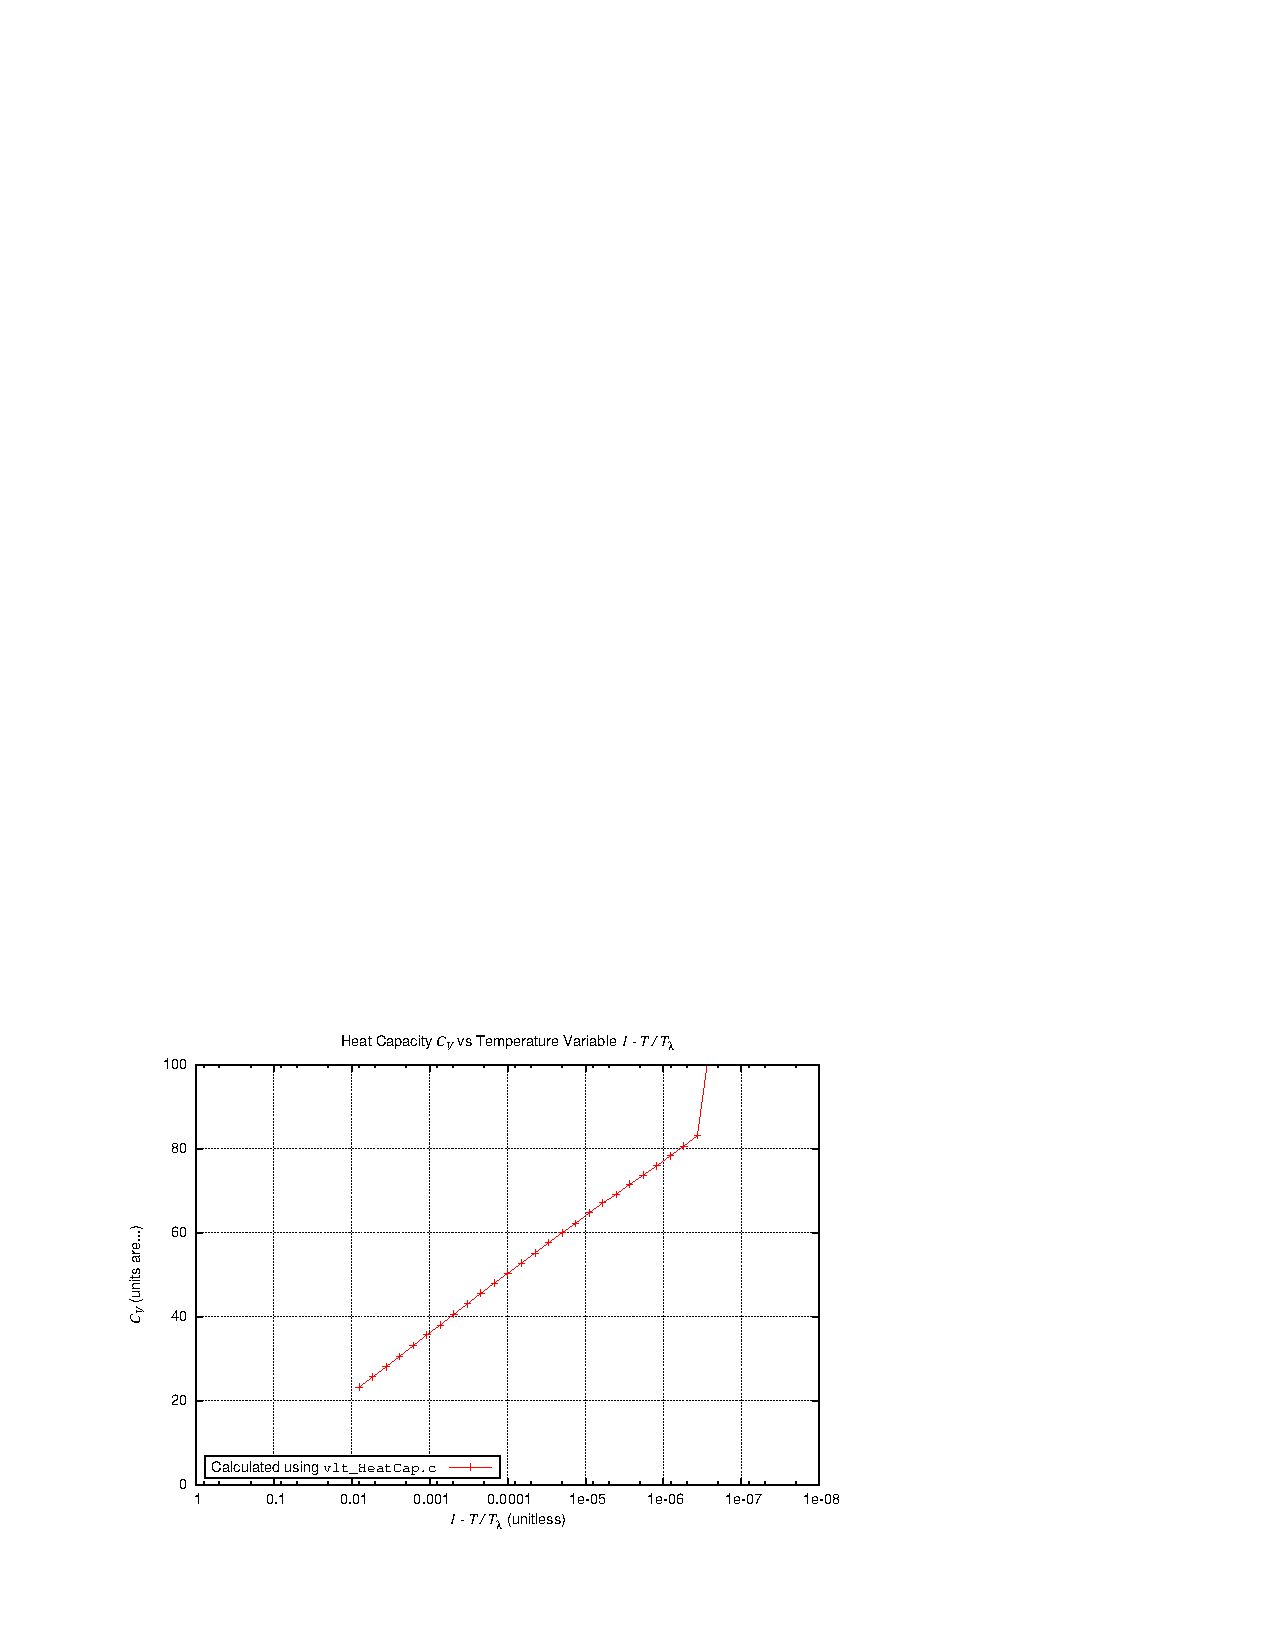
\includegraphics[width=8.5cm,viewport=54 53 410 300]{plot_HeatCapVsTempV_DK0110.pdf}\newline
  \verb|plot_HeatCapVsTempV_DK0110.pdf|
\else
  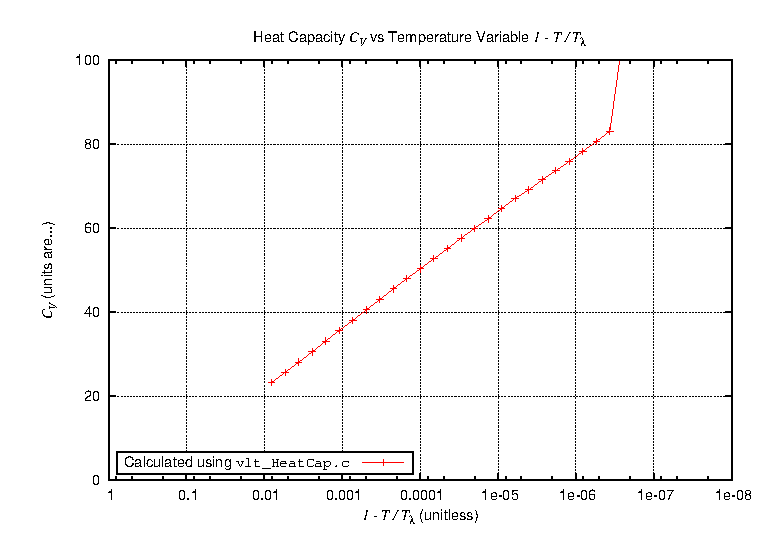
\includegraphics[width=8.5cm]{plot_HeatCapVsTempV_DK0110.ps}\newline
  \verb|plot_HeatCapVsTempV_DK0110.ps|
\fi
 \\
\ifpdf
  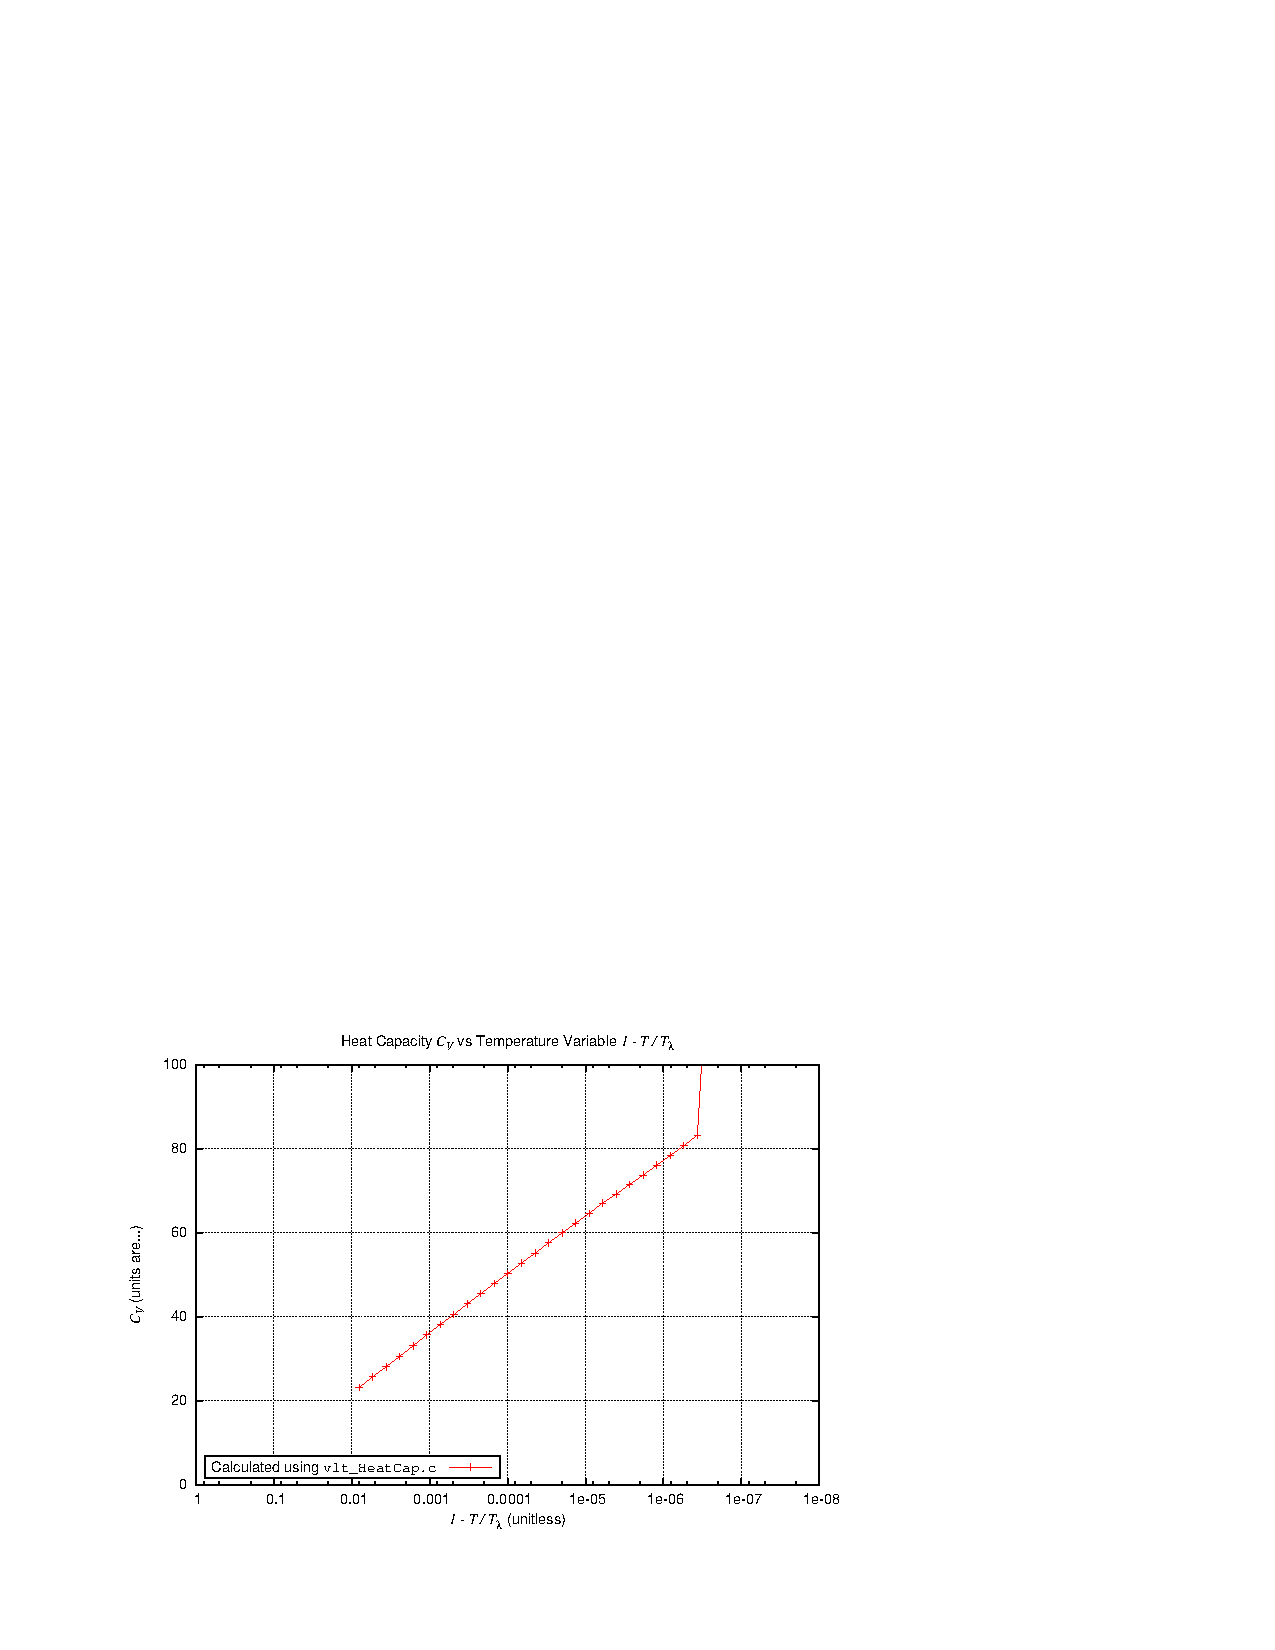
\includegraphics[width=8.5cm,viewport=54 53 410 300]{plot_HeatCapVsTempV_DK0120.pdf}\newline
  \verb|plot_HeatCapVsTempV_DK0120.pdf|
\else
  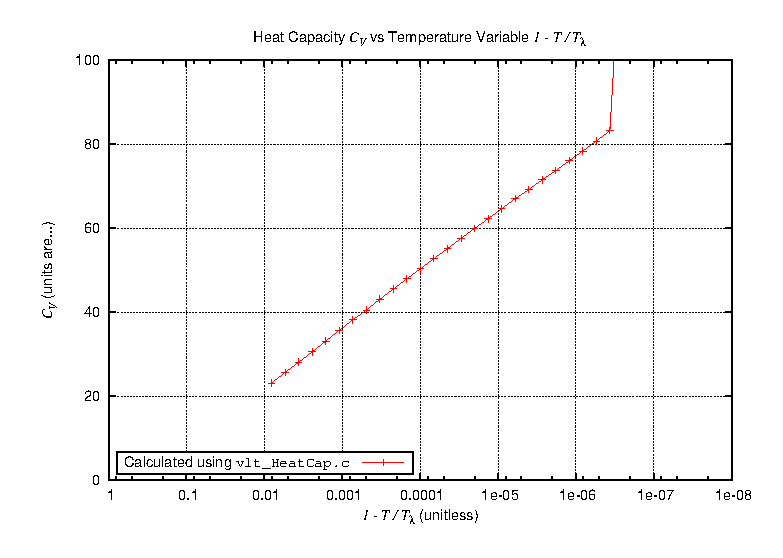
\includegraphics[width=8.5cm]{plot_HeatCapVsTempV_DK0120.ps}\newline
  \verb|plot_HeatCapVsTempV_DK0120.ps|
\fi
&
\ifpdf
  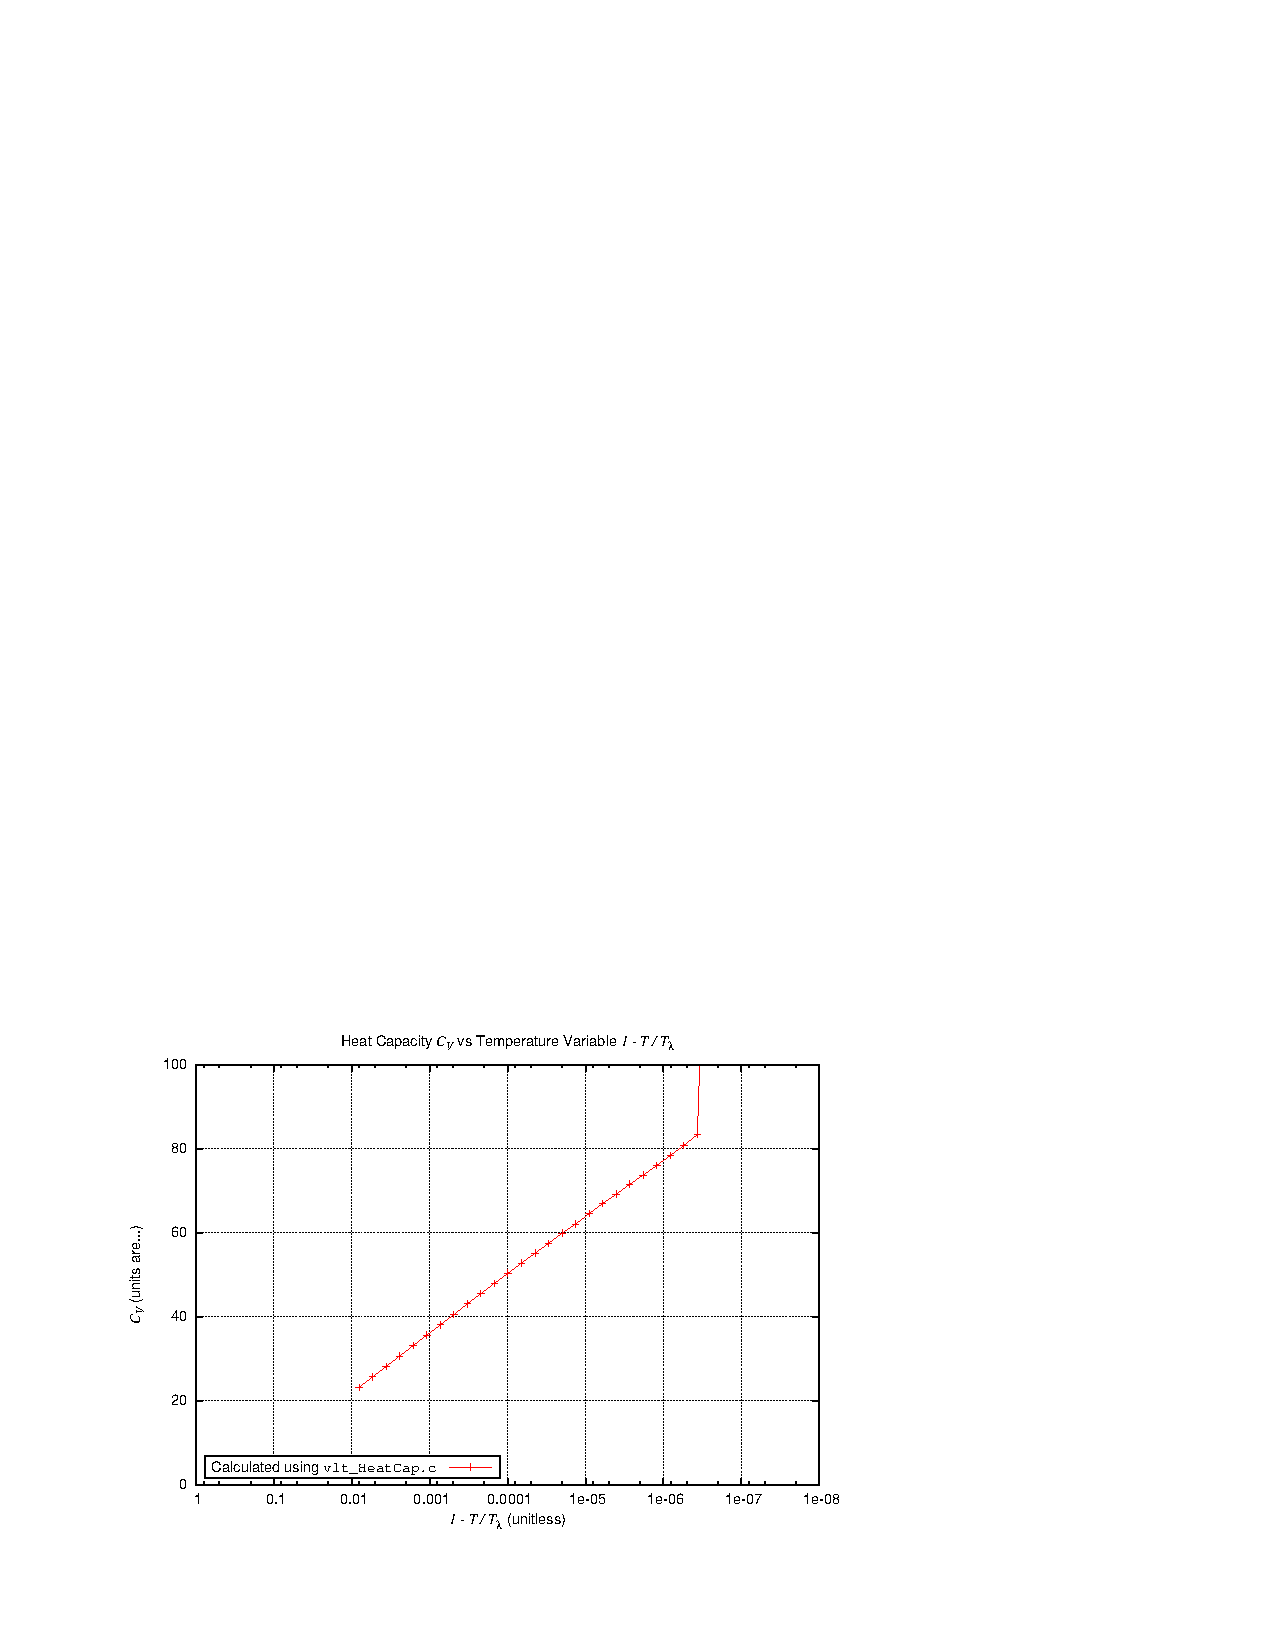
\includegraphics[width=8.5cm,viewport=54 53 410 300]{plot_HeatCapVsTempV_DK0130.pdf}\newline
  \verb|plot_HeatCapVsTempV_DK0130.pdf|
\else
  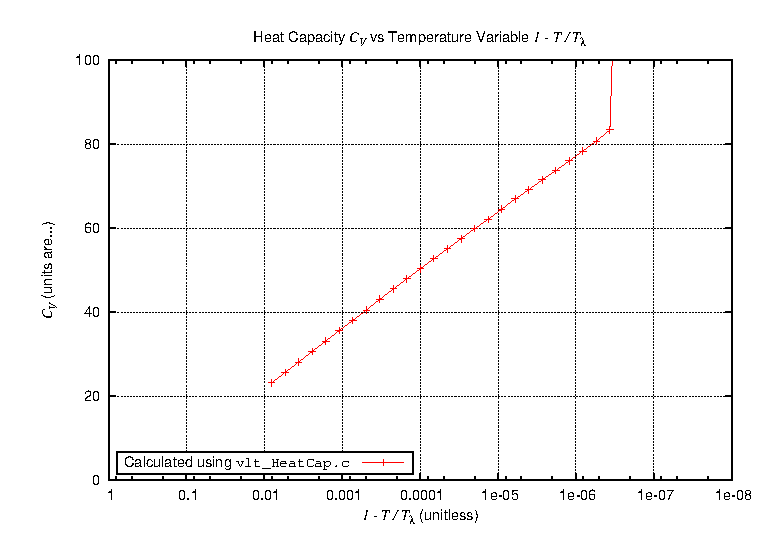
\includegraphics[width=8.5cm]{plot_HeatCapVsTempV_DK0130.ps}\newline
  \verb|plot_HeatCapVsTempV_DK0130.ps|
\fi
 \\
\end{tabular}
\end{center}


\begin{center}
\begin{tabular}[\textwidth]{p{8.5cm}p{8.5cm}}
\ifpdf
  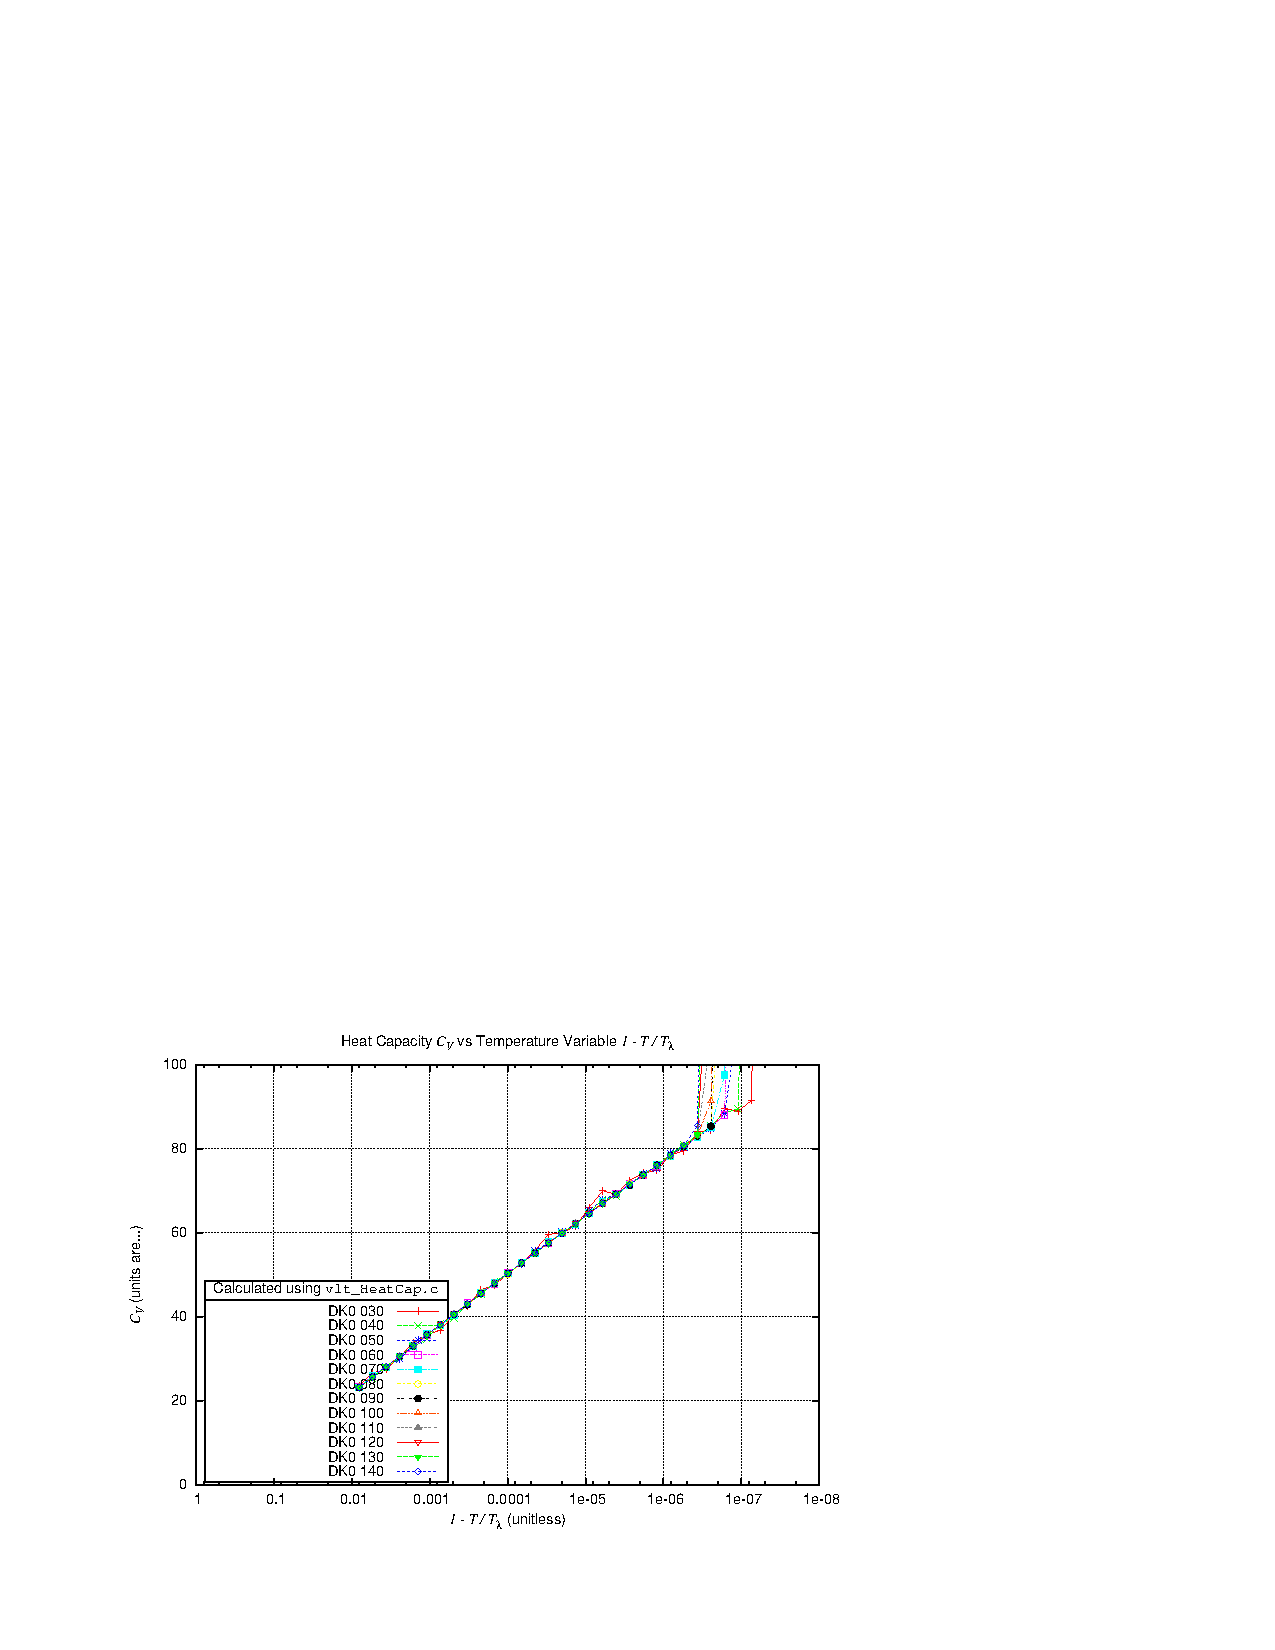
\includegraphics[width=8.5cm,viewport=54 53 410 300]{plot_HeatCapVsTempV_DK0140.pdf}\newline
  \verb|plot_HeatCapVsTempV_DK0140.pdf|
\else
  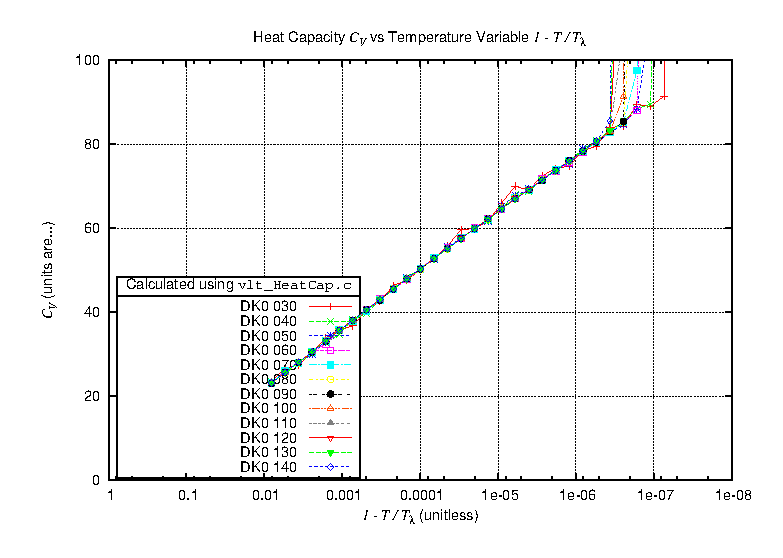
\includegraphics[width=8.5cm]{plot_HeatCapVsTempV_DK0140.ps}\newline
  \verb|plot_HeatCapVsTempV_DK0140.ps|
\fi
&
\ifpdf
  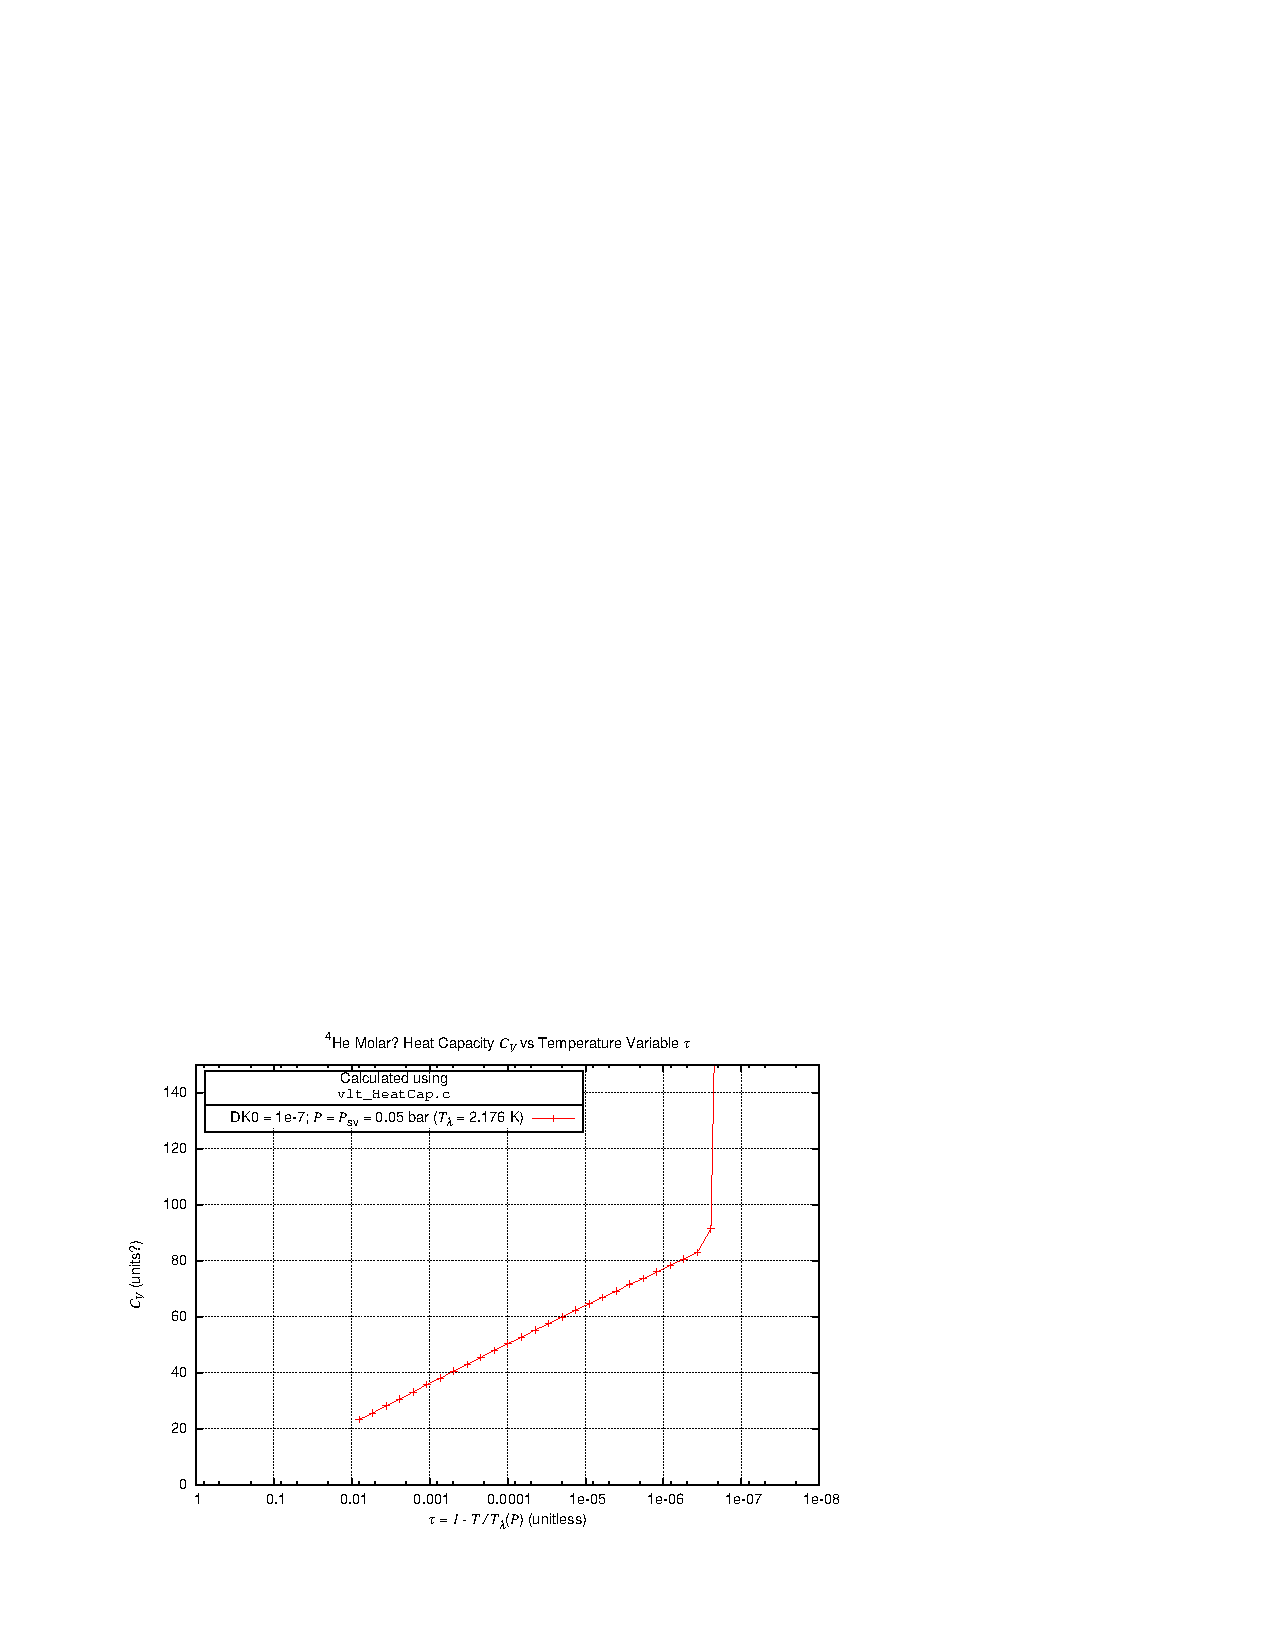
\includegraphics[width=8.5cm,viewport=54 53 410 300]{plot_HeatCapVsTvPress.pdf}\newline
  \verb|plot_HeatCapVsTvPress.pdf|
\else
  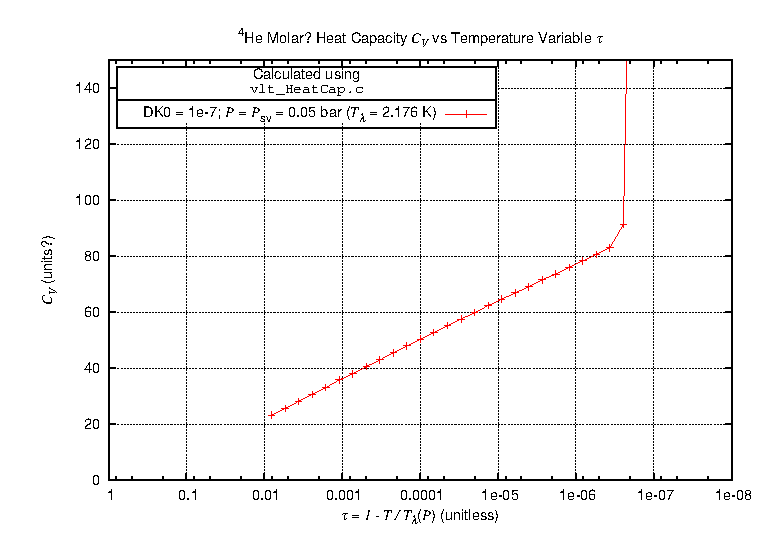
\includegraphics[width=8.5cm]{plot_HeatCapVsTvPress.ps}\newline
  \verb|plot_HeatCapVsTvPress.ps|
\fi
 \\
\end{tabular}
\end{center}

\end{comment}




\begin{center}
\begin{tabular}[\textwidth]{p{8.5cm}p{8.5cm}}
\ifpdf
  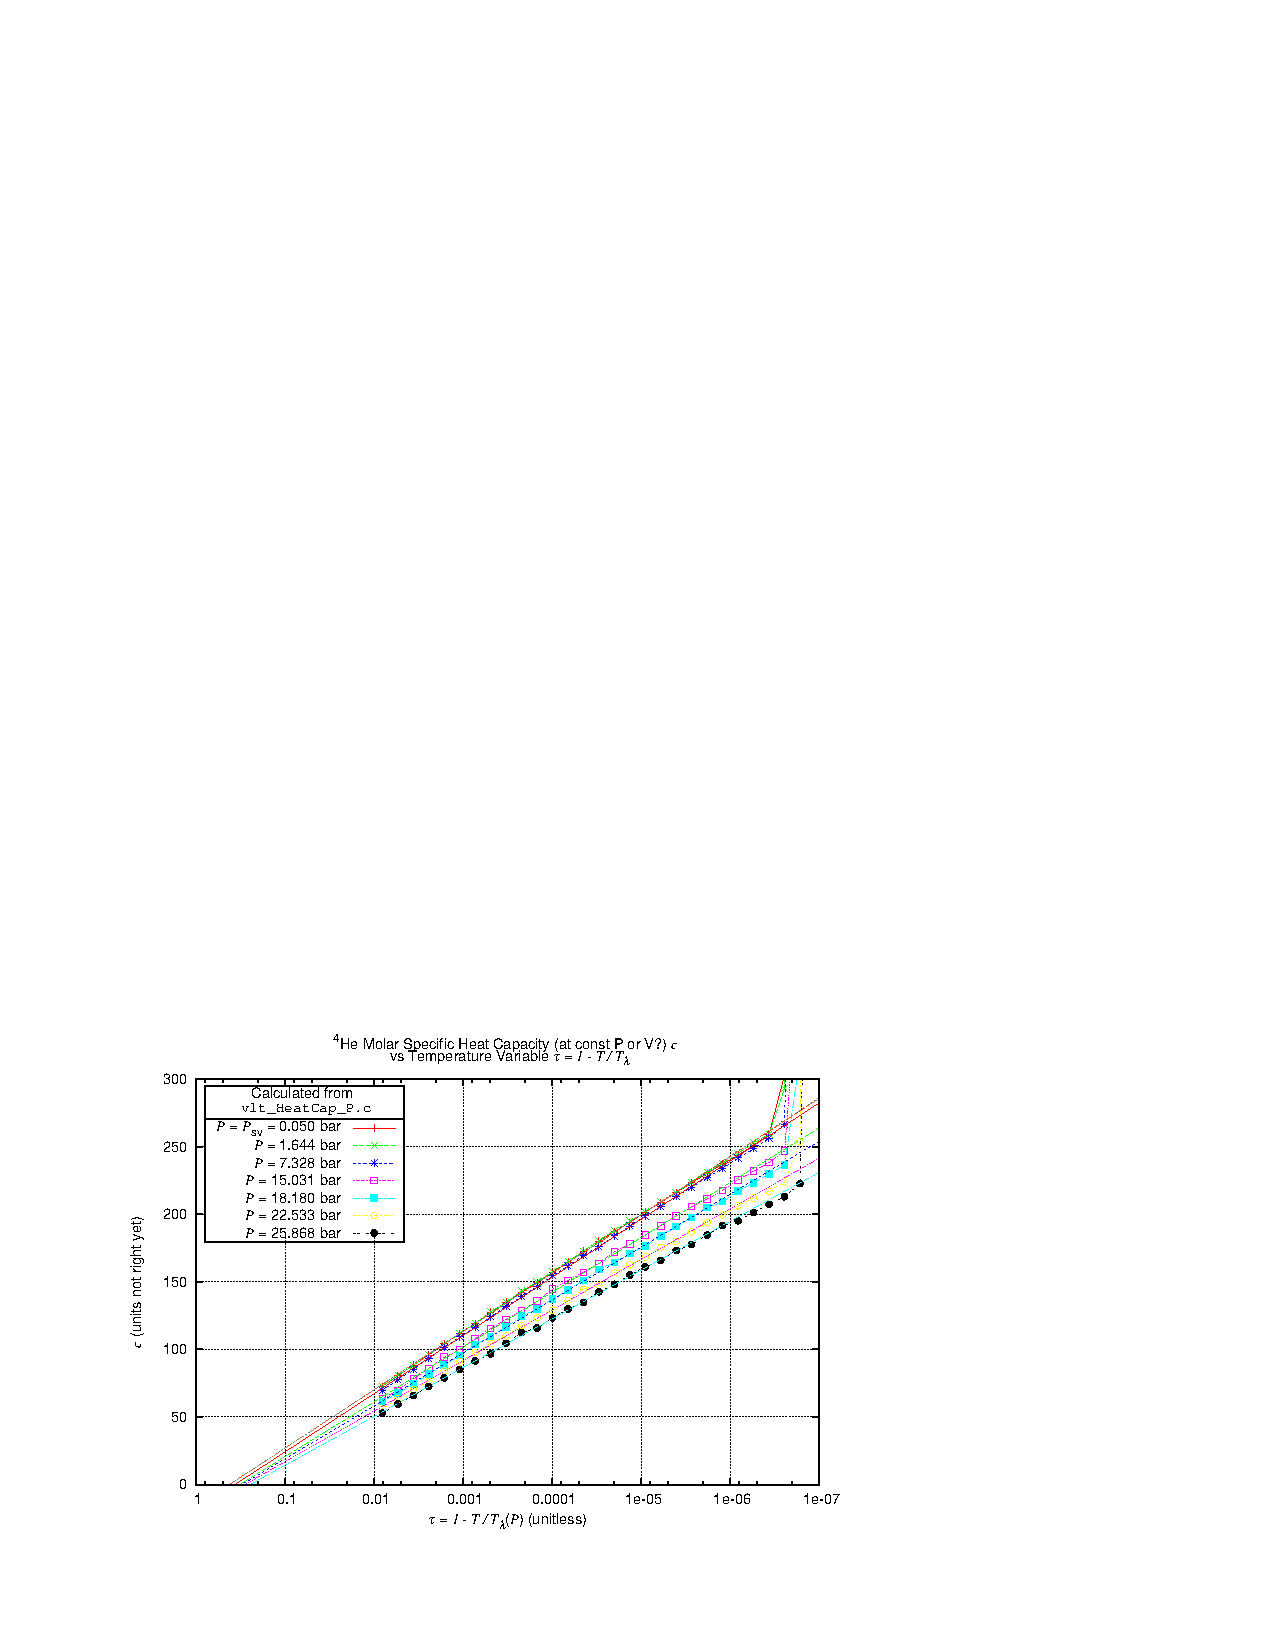
\includegraphics[width=8.5cm,viewport=54 53 410 300]{plot_vlt_HeatCap_P_DK0_1e-07_CapVsTv_log_AhlersCompare_adjust.pdf}\newline
  \verb|plot_vlt_HeatCap_P_DK0_1e-07_CapVsTv_log_| \newline \verb|AhlersCompare_adjust.pdf|
\else
  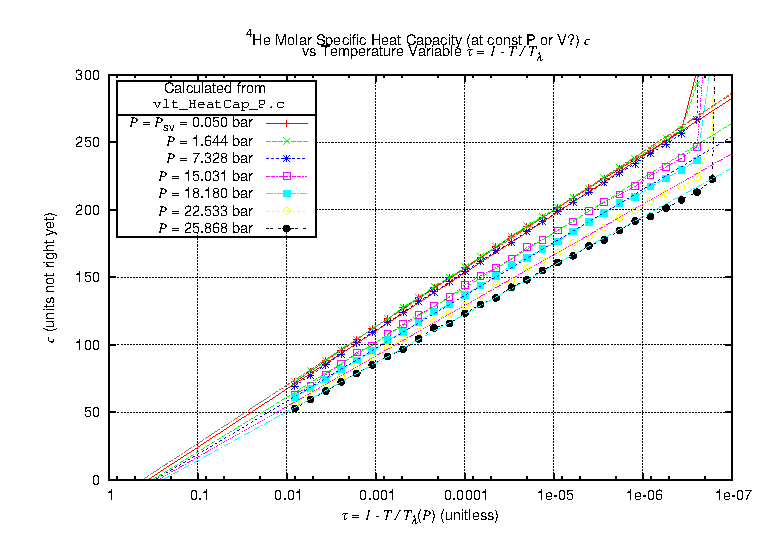
\includegraphics[width=8.5cm]{plot_vlt_HeatCap_P_DK0_1e-07_CapVsTv_log_AhlersCompare_adjust.ps}\newline
  \verb|plot_vlt_HeatCap_P_DK0_1e-07_CapVsTv_log_| \newline \verb|AhlersCompare_adjust.ps|
\fi
&
 \\
\end{tabular}
\end{center}



The following files are incorrect and so are not included (but can be shown if uncommented in \verb|ProgramPlots1.tex| file):
\squishlist
  \item \verb|plot_vlt_HeatCap_P_DK0_1e-07_CapVsTv_log_AhlersCompare.ps|
  \item \verb|plot_vlt_HeatCap_P_DK0_1e-07_CapVsTv_log.ps|
\squishend
\begin{comment}
\begin{center}
\begin{tabular}[\textwidth]{p{8.5cm}p{8.5cm}}
\ifpdf
  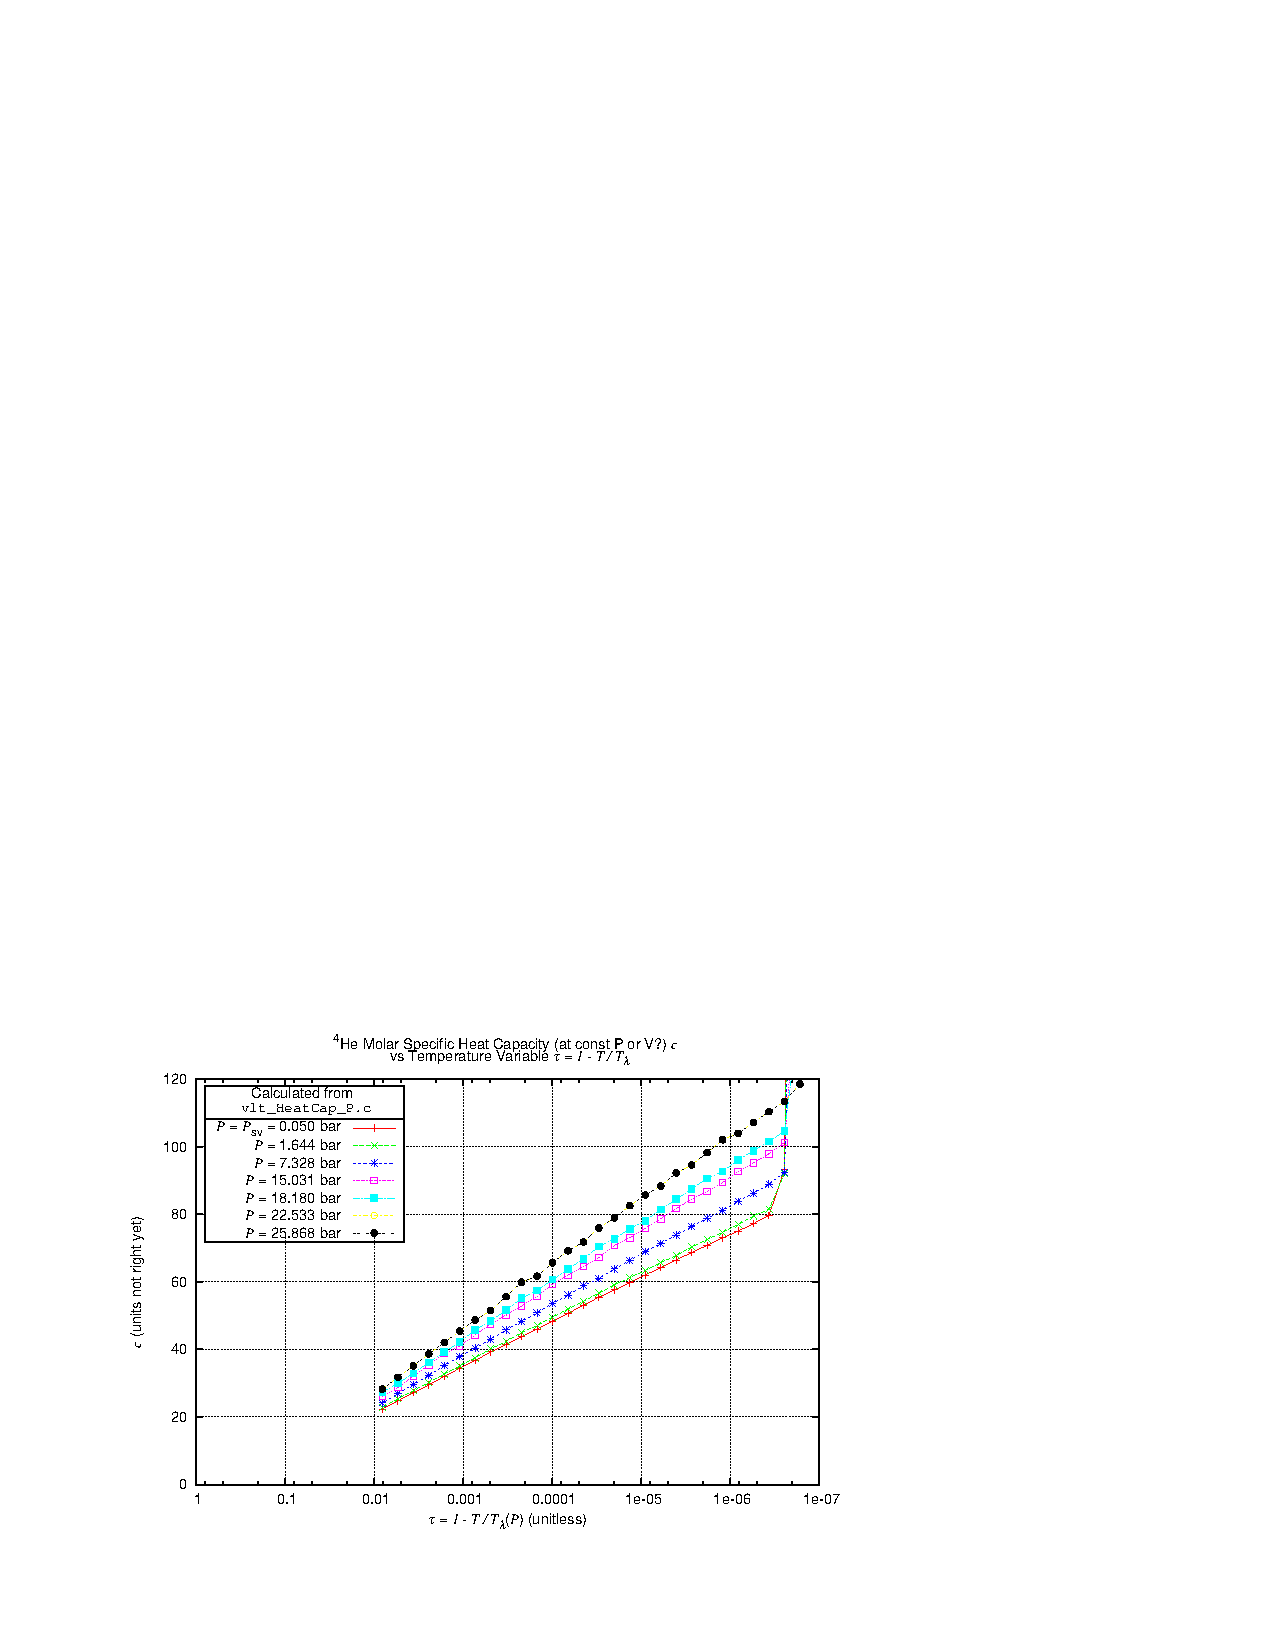
\includegraphics[width=8.5cm,viewport=54 53 410 300]{plot_vlt_HeatCap_P_DK0_1e-07_CapVsTv_log_AhlersCompare.pdf}\newline
  \verb|plot_vlt_HeatCap_P_DK0_1e-07_CapVsTv_log_| \newline \verb|AhlersCompare.pdf|
\else
  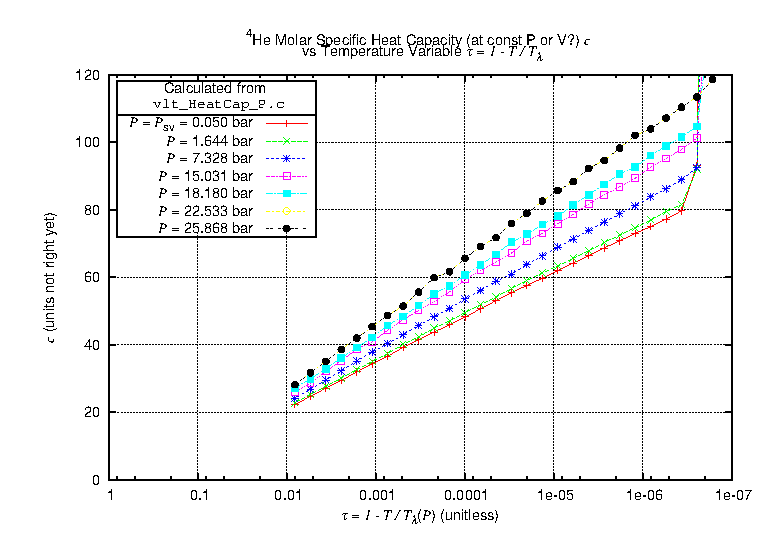
\includegraphics[width=8.5cm]{plot_vlt_HeatCap_P_DK0_1e-07_CapVsTv_log_AhlersCompare.ps}\newline
  \verb|plot_vlt_HeatCap_P_DK0_1e-07_CapVsTv_log_| \newline \verb|AhlersCompare.ps|
\fi
&
\ifpdf
  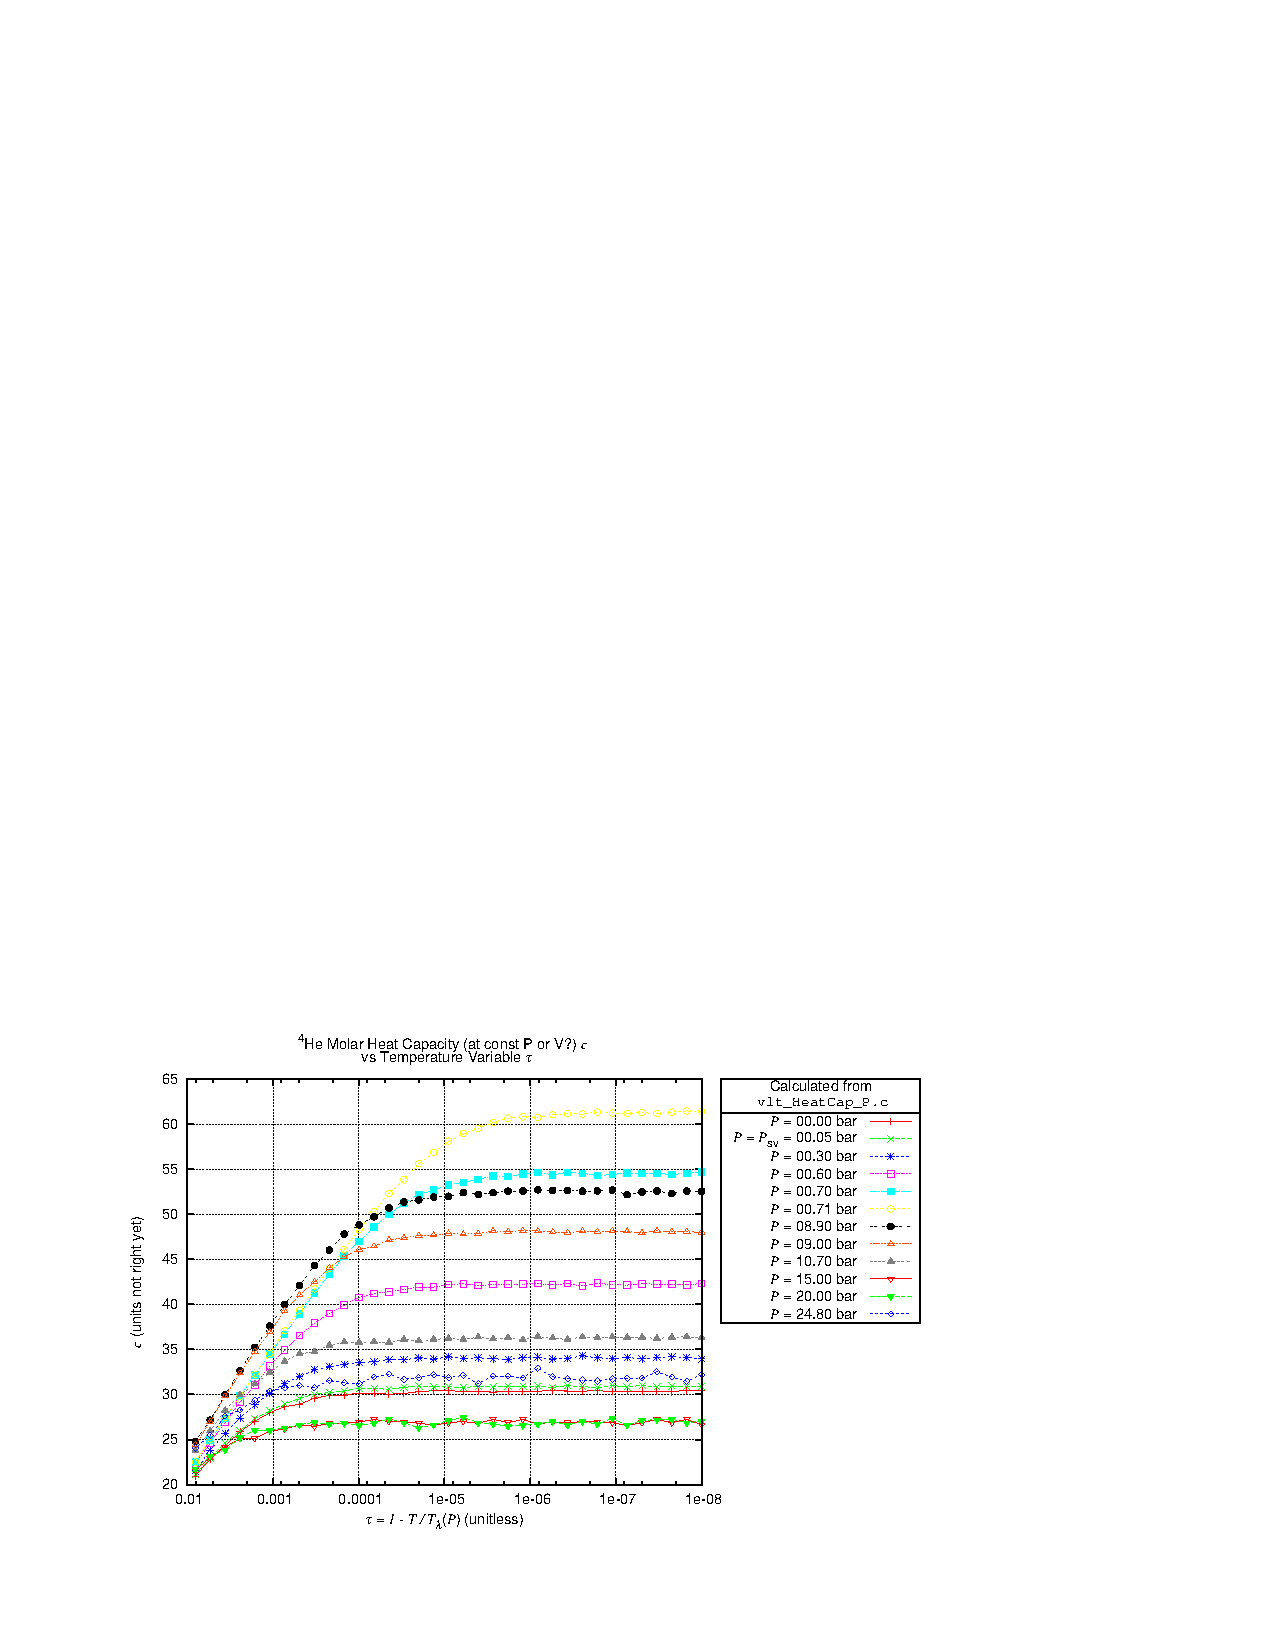
\includegraphics[width=8.5cm,viewport=54 53 410 300]{plot_vlt_HeatCap_P_DK0_1e-07_CapVsTv_log.pdf}\newline
  \verb|plot_vlt_HeatCap_P_DK0_1e-07_CapVsTv_log.pdf|
\else
  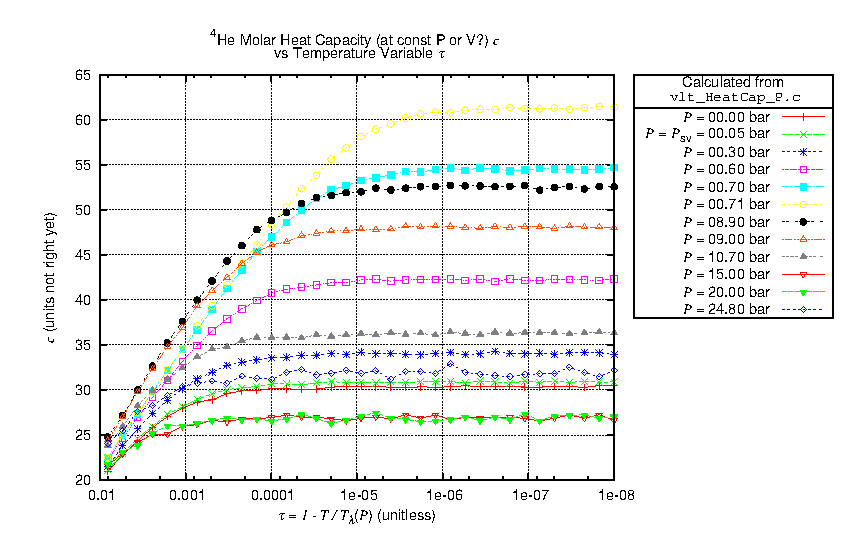
\includegraphics[width=8.5cm]{plot_vlt_HeatCap_P_DK0_1e-07_CapVsTv_log.ps}\newline
  \verb|plot_vlt_HeatCap_P_DK0_1e-07_CapVsTv_log.ps|
\fi
 \\
\ifpdf
  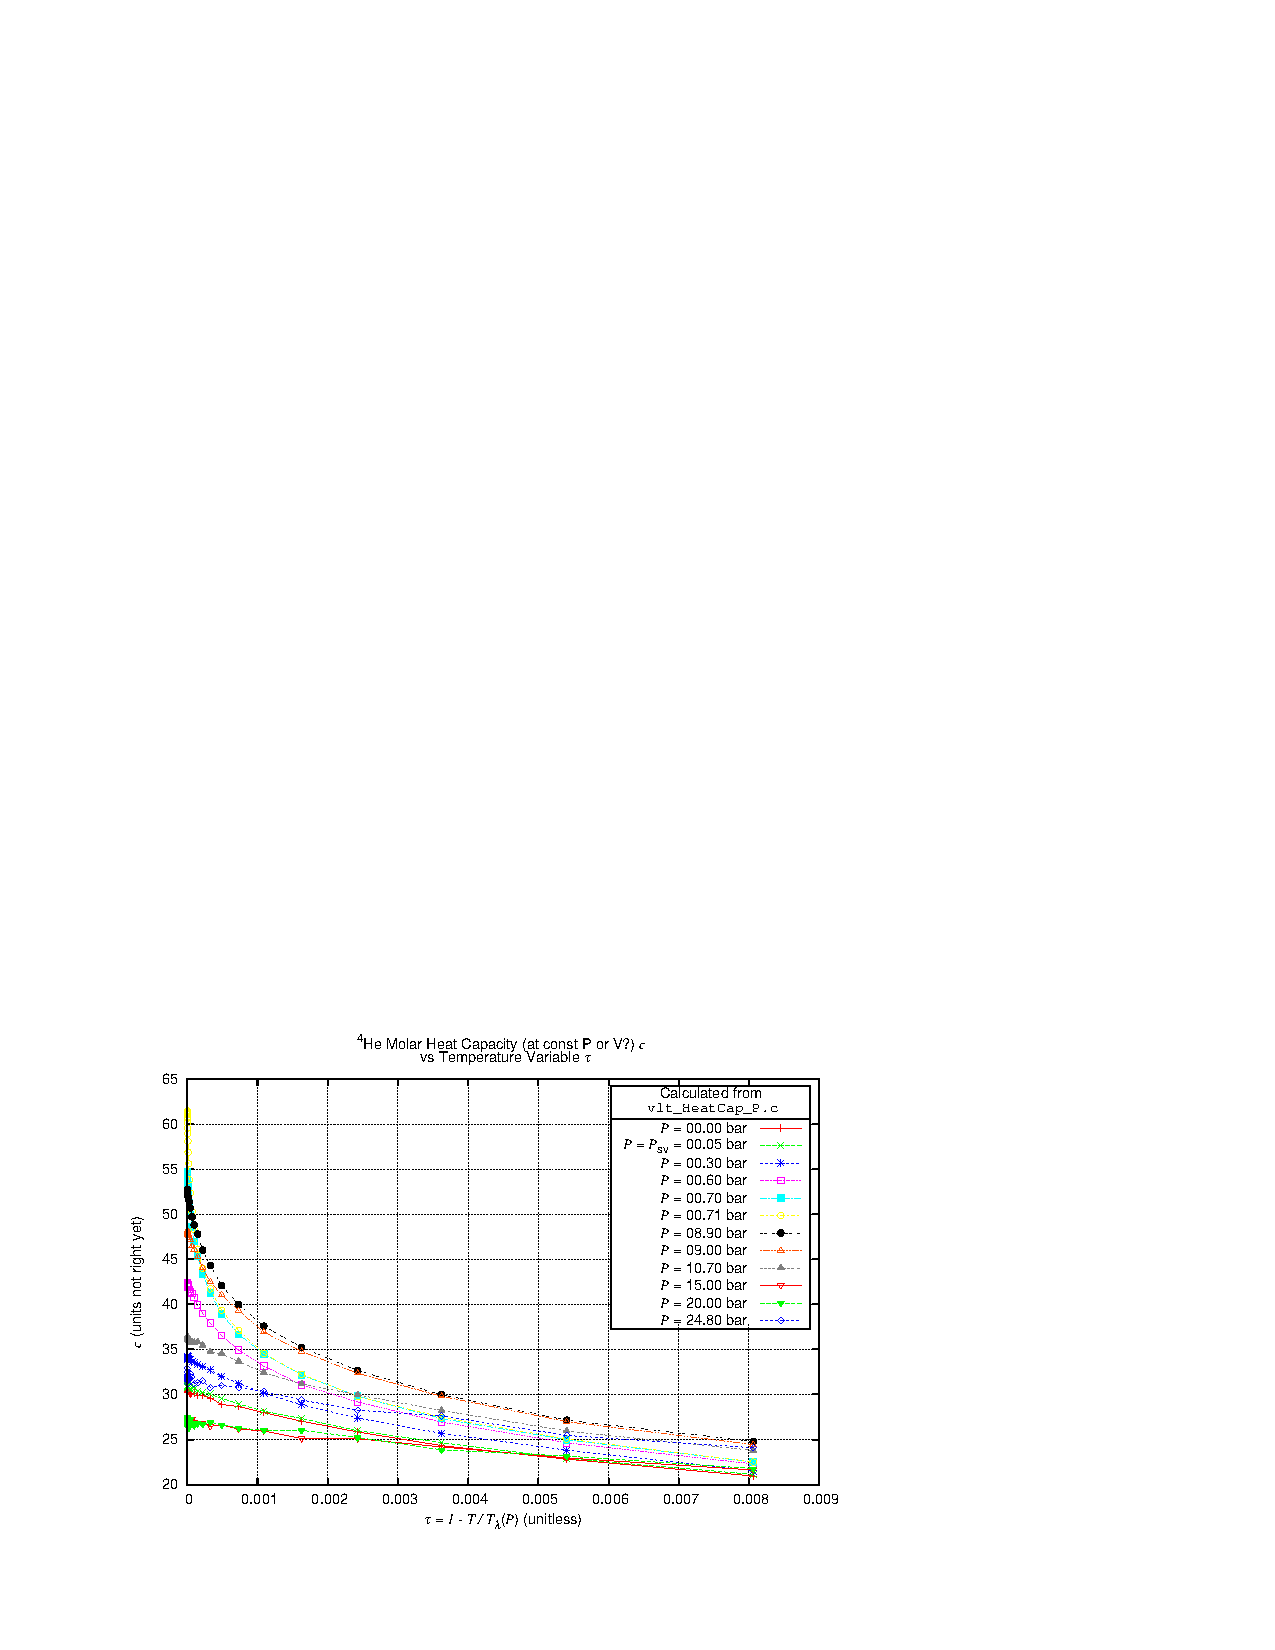
\includegraphics[width=8.5cm,viewport=54 53 410 300]{plot_vlt_HeatCap_P_DK0_1e-07_CapVsTv.pdf}\newline
  \verb|plot_vlt_HeatCap_P_DK0_1e-07_CapVsTv.pdf|
\else
  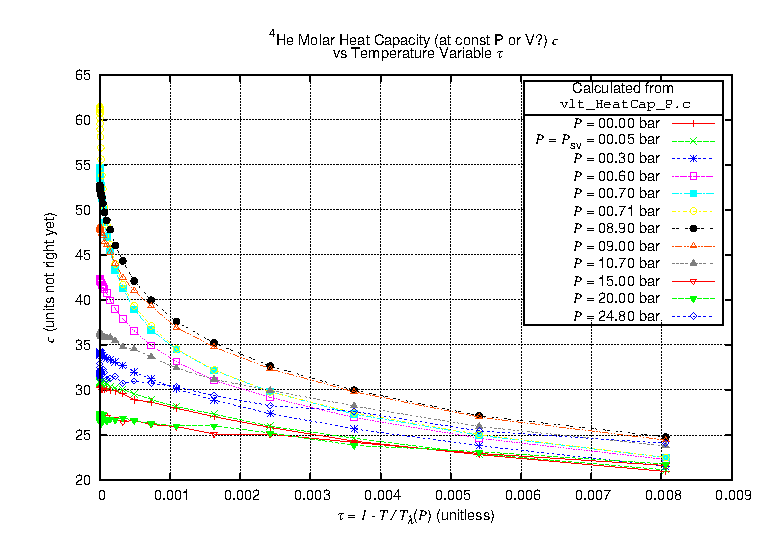
\includegraphics[width=8.5cm]{plot_vlt_HeatCap_P_DK0_1e-07_CapVsTv.ps}\newline
  \verb|plot_vlt_HeatCap_P_DK0_1e-07_CapVsTv.ps|
\fi
&
 \\
\end{tabular}
\end{center}
\end{comment}



\begin{center}
\begin{tabular}[\textwidth]{p{8.5cm}p{8.5cm}}
\ifpdf
  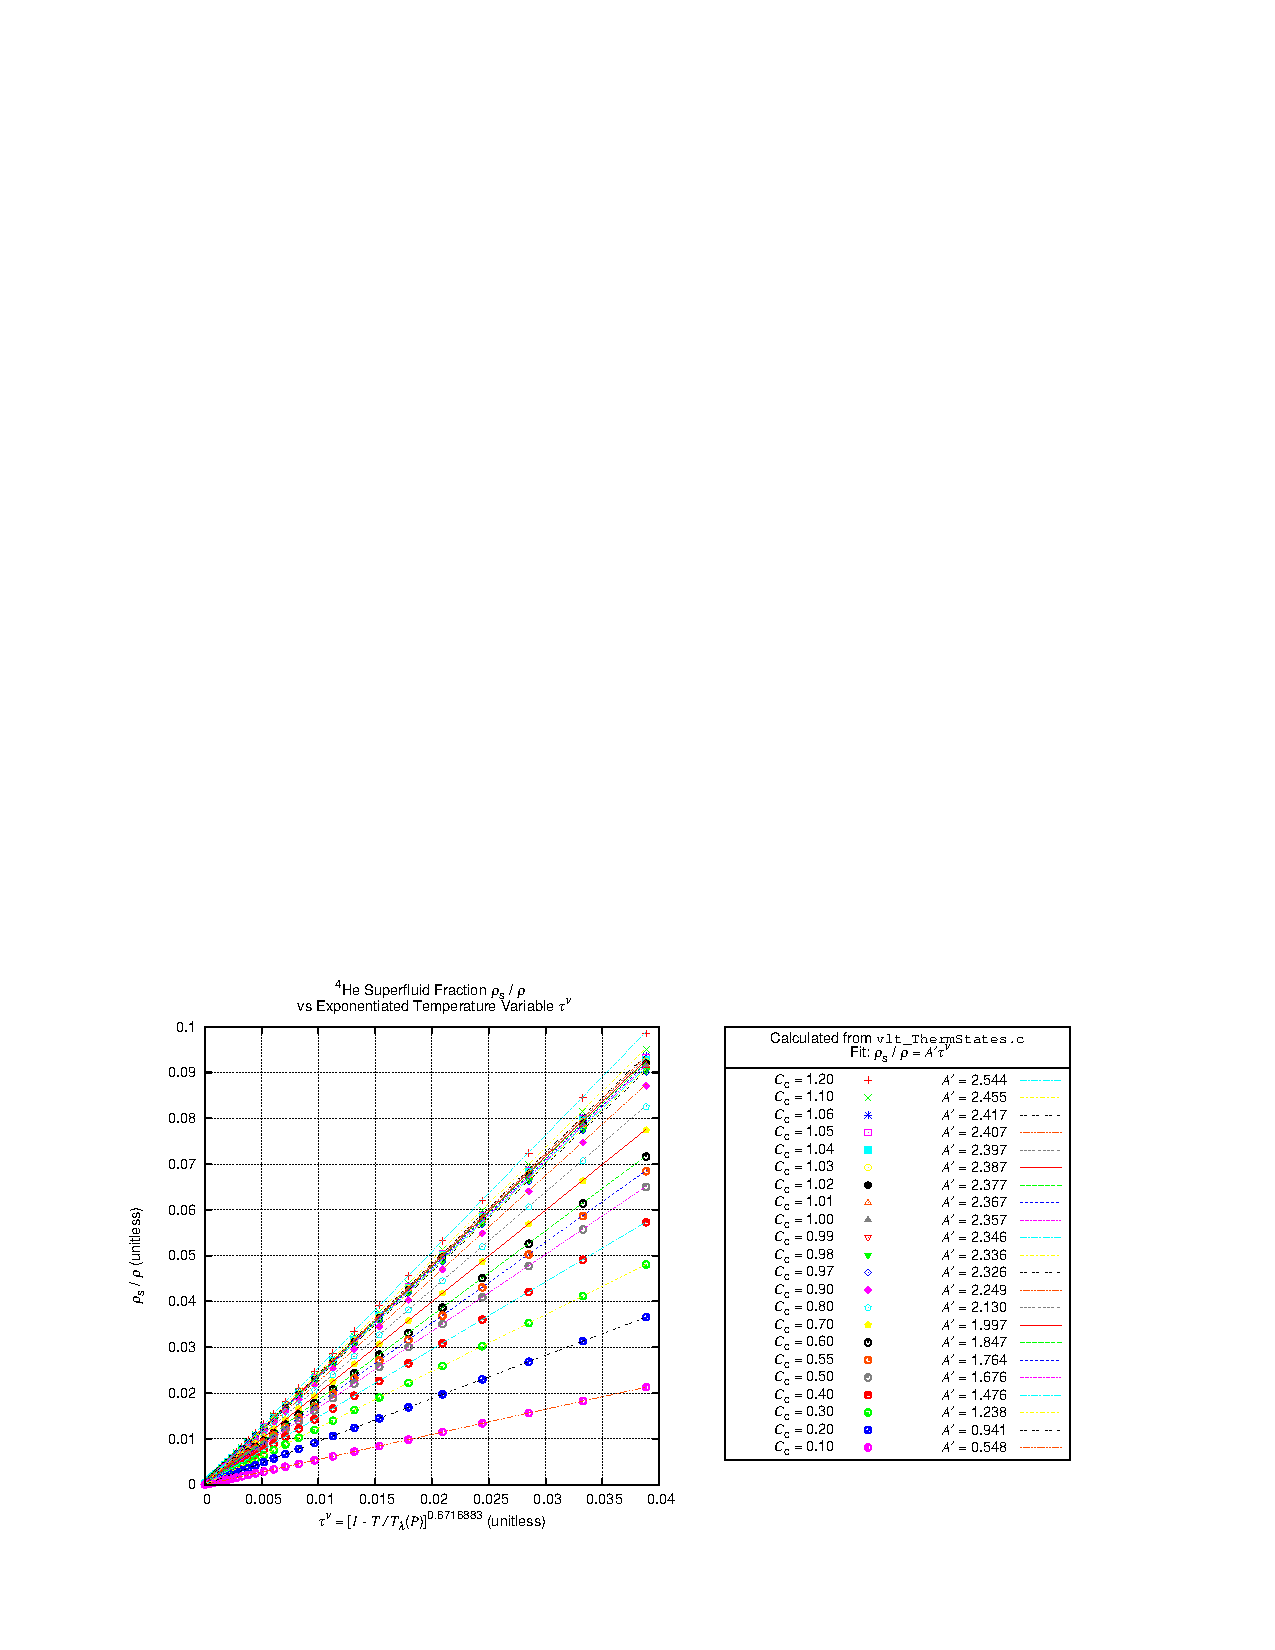
\includegraphics[width=8.5cm,viewport=54 53 410 300]{plot_vlt_ThermStates_Dexp100_A_RhosoRhoVsTvNu.pdf}\newline
  \verb|plot_vlt_ThermStates_Dexp100_A_RhosoRhoVsTvNu.pdf|
\else
  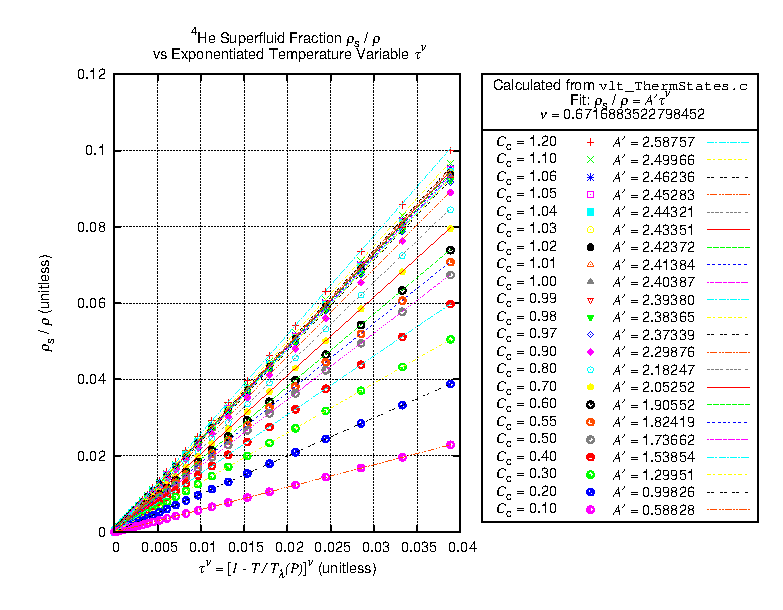
\includegraphics[width=8.5cm]{plot_vlt_ThermStates_Dexp100_A_RhosoRhoVsTvNu.ps}\newline
  \verb|plot_vlt_ThermStates_Dexp100_A_RhosoRhoVsTvNu.ps|
\fi
&
 \\
\end{tabular}
\end{center}









\newpage
\section{Adjusted Theory}

These plots use data from \verb|ring3.c|, \verb|derk1.c|, and \verb|Donnelly_rhos.dat|.  Option \verb|beta| in \verb|ring3.c| was created using data points placed in \verb|funkyfactorfit.dat| designed to make a smooth transition in the plot of \verb|plot_ring3_Delok_beta.png| from about $\unit{8.68}{\kelvin}$ to $\unit{6.8}{\kelvin}$.  (See \verb|HeliumDensities.ods| in the \verb|supporting| folder for calculations and plots of ``\verb|Del/kB 3|''.)

\begin{center}
\begin{tabular}[\textwidth]{p{8.5cm}p{8.5cm}}
\ifpdf
  \includegraphics[width=8.5cm]{plot_rhos_compare_alpha.png}\newline
  \verb|plot_rhos_compare_alpha.png|
\else
  \includegraphics[width=8.5cm]{plot_rhos_compare_alpha.eps}\newline
  \verb|plot_rhos_compare_alpha.eps|
\fi
&
\ifpdf
  \includegraphics[width=8.5cm]{plot_ring3_Delok_alpha.png}\newline
  \verb|plot_ring3_Delok_alpha.png|
\else
  \includegraphics[width=8.5cm]{plot_ring3_Delok_alpha.eps}\newline
  \verb|plot_ring3_Delok_alpha.eps|
\fi
 \\
\ifpdf
  \includegraphics[width=8.5cm]{plot_rhos_compare_beta.png}\newline
  \verb|plot_rhos_compare_beta.png|
\else
  \includegraphics[width=8.5cm]{plot_rhos_compare_beta.eps}\newline
  \verb|plot_rhos_compare_beta.eps|
\fi
&
\ifpdf
  \includegraphics[width=8.5cm]{plot_ring3_Delok_beta.png}\newline
  \verb|plot_ring3_Delok_beta.png|
\else
  \includegraphics[width=8.5cm]{plot_ring3_Delok_beta.eps}\newline
  \verb|plot_ring3_Delok_beta.eps|
\fi
 \\
\end{tabular}
\end{center}




\newpage
\section{Initial Theory}

\subsection{2D Program Plots}

These plots use data from \verb|2DKT.c| and \verb|derk1.c|.

\subsubsection{Major Plots}

\begin{tabular}[\textwidth]{p{8.5cm}p{8.5cm}}
\ifpdf
  \includegraphics[width=8.5cm]{plot_2D_KrK0versusl_B_linlin.png}\newline
  \verb|plot_2D_KrK0versusl_B_linlin.png|
\else
  \includegraphics[width=8.5cm]{plot_2D_KrK0versusl_B_linlin.eps}\newline
  \verb|plot_2D_KrK0versusl_B_linlin.eps|
\fi
&
\ifpdf
  \includegraphics[width=8.5cm]{plot_2D_KrK0versusT_B_linlin.png}\newline
  \verb|plot_2D_KrK0versusT_B_linlin.png|
\else
  \includegraphics[width=8.5cm]{plot_2D_KrK0versusT_B_linlin.eps}\newline
  \verb|plot_2D_KrK0versusT_B_linlin.eps|
\fi
 \\
\ifpdf
  \includegraphics[width=8.5cm]{plot_2D_yversusl_B_loglin.png}\newline
  \verb|plot_2D_yversusl_B_loglin.png|
\else
  \includegraphics[width=8.5cm]{plot_2D_yversusl_B_loglin.eps}\newline
  \verb|plot_2D_yversusl_B_loglin.eps|
\fi
&
\ifpdf
  \includegraphics[width=8.5cm]{plot_2D_yversusT_B_loglin.png}\newline
  \verb|plot_2D_yversusT_B_loglin.png|
\else
  \includegraphics[width=8.5cm]{plot_2D_yversusT_B_loglin.eps}\newline
  \verb|plot_2D_yversusT_B_loglin.eps|
\fi
 \\
\end{tabular}




\subsubsection{Minor Plots}

\begin{tabular}[\textwidth]{p{8.5cm}p{8.5cm}}
\ifpdf
  \includegraphics[width=8.5cm]{plot_2D_KrversusT_A_linlin.png}\newline
  \verb|plot_2D_KrversusT_A_linlin.png|
\else
  \includegraphics[width=8.5cm]{plot_2D_KrversusT_A_linlin.eps}\newline
  \verb|plot_2D_KrversusT_A_linlin.eps|
\fi
&
\ifpdf
  \includegraphics[width=8.5cm]{plot_2D_KrversusT_B_linlin.png}\newline
  \verb|plot_2D_KrversusT_B_linlin.png|
\else
  \includegraphics[width=8.5cm]{plot_2D_KrversusT_B_linlin.eps}\newline
  \verb|plot_2D_KrversusT_B_linlin.eps|
\fi
 \\
\ifpdf
  \includegraphics[width=8.5cm]{plot_2D_Kversusl_A_loglin.png}\newline
  \verb|plot_2D_Kversusl_A_loglin.png|
\else
  \includegraphics[width=8.5cm]{plot_2D_Kversusl_A_loglin.eps}\newline
  \verb|plot_2D_Kversusl_A_loglin.eps|
\fi
&
\ifpdf
  \includegraphics[width=8.5cm]{plot_2D_Kversusl_B_linlin.png}\newline
  \verb|plot_2D_Kversusl_B_linlin.png|
\else
  \includegraphics[width=8.5cm]{plot_2D_Kversusl_B_linlin.eps}\newline
  \verb|plot_2D_Kversusl_B_linlin.eps|
\fi
 \\
\end{tabular}




\newpage
\subsection{3D Program Plots}

These plots use data from \verb|ring1.c| and \verb|derk1.c|.

\subsubsection{Major Plots}

\begin{tabular}[\textwidth]{p{8.5cm}p{8.5cm}}
\ifpdf
  \includegraphics[width=8.5cm]{plot_3D_KrK0versusl_B_linlin.png}\newline
  \verb|plot_3D_KrK0versusl_B_linlin.png|
\else
  \includegraphics[width=8.5cm]{plot_3D_KrK0versusl_B_linlin.eps}\newline
  \verb|plot_3D_KrK0versusl_B_linlin.eps|
\fi
&
\ifpdf
  \includegraphics[width=8.5cm]{plot_3D_KrK0versusT_B_linlin.png}\newline
  \verb|plot_3D_KrK0versusT_B_linlin.png|
\else
  \includegraphics[width=8.5cm]{plot_3D_KrK0versusT_B_linlin.eps}\newline
  \verb|plot_3D_KrK0versusT_B_linlin.eps|
\fi
 \\
\ifpdf
  \includegraphics[width=8.5cm]{plot_3D_yversusl_B_linlin.png}\newline
  \verb|plot_3D_yversusl_B_linlin.png|
\else
  \includegraphics[width=8.5cm]{plot_3D_yversusl_B_linlin.eps}\newline
  \verb|plot_3D_yversusl_B_linlin.eps|
\fi
&
\ifpdf
  \includegraphics[width=8.5cm]{plot_3D_yversusT_B_linlin.png}\newline
  \verb|plot_3D_yversusT_B_linlin.png|
\else
  \includegraphics[width=8.5cm]{plot_3D_yversusT_B_linlin.eps}\newline
  \verb|plot_3D_yversusT_B_linlin.eps|
\fi
 \\
\ifpdf
  \includegraphics[width=8.5cm]{plot_3D_Fversusl_B_linlin.png}\newline
  \verb|plot_3D_Fversusl_B_linlin.png|
\else
  \includegraphics[width=8.5cm]{plot_3D_Fversusl_B_linlin.eps}\newline
  \verb|plot_3D_Fversusl_B_linlin.eps|
\fi
&
\ifpdf
  \includegraphics[width=8.5cm]{plot_3D_FversusT_B_linlin.png}\newline
  \verb|plot_3D_FversusT_B_linlin.png|
\else
  \includegraphics[width=8.5cm]{plot_3D_FversusT_B_linlin.eps}\newline
  \verb|plot_3D_FversusT_B_linlin.eps|
\fi
 \\
\end{tabular}


\subsubsection{Minor Plots}

\begin{tabular}[\textwidth]{p{8.5cm}p{8.5cm}}
\ifpdf
  \includegraphics[width=8.5cm]{plot_3D_KrK0versusl_A_loglog.png}\newline
  \verb|plot_3D_KrK0versusl_A_loglog.png|
\else
  \includegraphics[width=8.5cm]{plot_3D_KrK0versusl_A_loglog.eps}\newline
  \verb|plot_3D_KrK0versusl_A_loglog.eps|
\fi
&
\ifpdf
  \includegraphics[width=8.5cm]{plot_3D_KrK0versusl_B_loglog.png}\newline
  \verb|plot_3D_KrK0versusl_B_loglog.png|
\else
  \includegraphics[width=8.5cm]{plot_3D_KrK0versusl_B_loglog.eps}\newline
  \verb|plot_3D_KrK0versusl_B_loglog.eps|
\fi
 \\
\ifpdf
  \includegraphics[width=8.5cm]{plot_3D_KrK0versusTv_A_loglog.png}\newline
  \verb|plot_3D_KrK0versusTv_A_loglog.png|
\else
  \includegraphics[width=8.5cm]{plot_3D_KrK0versusTv_A_loglog.eps}\newline
  \verb|plot_3D_KrK0versusTv_A_loglog.eps|
\fi
&
\ifpdf
  \includegraphics[width=8.5cm]{plot_3D_KrK0versusTv_B_loglog.png}\newline
  \verb|plot_3D_KrK0versusTv_B_loglog.png|
\else
  \includegraphics[width=8.5cm]{plot_3D_KrK0versusTv_B_loglog.eps}\newline
  \verb|plot_3D_KrK0versusTv_B_loglog.eps|
\fi
 \\
\ifpdf
  \includegraphics[width=8.5cm]{plot_3D_KrversusT_B_linlin.png}\newline
  \verb|plot_3D_KrversusT_B_linlin.png|
\else
  \includegraphics[width=8.5cm]{plot_3D_KrversusT_B_linlin.eps}\newline
  \verb|plot_3D_KrversusT_B_linlin.eps|
\fi
&
\ifpdf
  \includegraphics[width=8.5cm]{plot_3D_Kversusl_A_loglin.png}\newline
  \verb|plot_3D_Kversusl_A_loglin.png|
\else
  \includegraphics[width=8.5cm]{plot_3D_Kversusl_A_loglin.eps}\newline
  \verb|plot_3D_Kversusl_A_loglin.eps|
\fi
 \\
\end{tabular}


\begin{tabular}[\textwidth]{p{8.5cm}p{8.5cm}}
\ifpdf
  \includegraphics[width=8.5cm]{plot_3D_KrK0versusTv_A_findA.png}\newline
  \verb|plot_3D_KrK0versusTv_A_findA.png|
\else
  \includegraphics[width=8.5cm]{plot_3D_KrK0versusTv_A_findA.eps}\newline
  \verb|plot_3D_KrK0versusTv_A_findA.eps|
\fi
&
\ifpdf
  \includegraphics[width=8.5cm]{plot_3D_KrK0versusTv_B_findA.png}\newline
  \verb|plot_3D_KrK0versusTv_B_findA.png|
\else
  \includegraphics[width=8.5cm]{plot_3D_KrK0versusTv_B_findA.eps}\newline
  \verb|plot_3D_KrK0versusTv_B_findA.eps|
\fi
 \\
\end{tabular}




\begin{tabular}[\textwidth]{p{8.5cm}p{8.5cm}}
\ifpdf
  \includegraphics[width=8.5cm]{plot_3D_Kversusl_A_loglog.png}\newline
  \verb|plot_3D_Kversusl_A_loglog.png|
\else
  \includegraphics[width=8.5cm]{plot_3D_Kversusl_A_loglog.eps}\newline
  \verb|plot_3D_Kversusl_A_loglog.eps|
\fi
&
\ifpdf
  \includegraphics[width=8.5cm]{plot_3D_Kversusl_B_linlin.png}\newline
  \verb|plot_3D_Kversusl_B_linlin.png|
\else
  \includegraphics[width=8.5cm]{plot_3D_Kversusl_B_linlin.eps}\newline
  \verb|plot_3D_Kversusl_B_linlin.eps|
\fi
 \\
\ifpdf
  \includegraphics[width=8.5cm]{plot_3D_yversusl_A_loglog.png}\newline
  \verb|plot_3D_yversusl_A_loglog.png|
\else
  \includegraphics[width=8.5cm]{plot_3D_yversusl_A_loglog.eps}\newline
  \verb|plot_3D_yversusl_A_loglog.eps|
\fi
& \\
\end{tabular}


\begin{tabular}[\textwidth]{p{8.5cm}p{8.5cm}}
\ifpdf
  \includegraphics[width=8.5cm]{plot_ring3_A_KrK0versusTv.png}\newline
  \verb|plot_ring3_A_KrK0versusTv.png|
\else
  \includegraphics[width=8.5cm]{plot_ring3_A_KrK0versusTv.eps}\newline
  \verb|plot_ring3_A_KrK0versusTv.eps|
\fi
&
\ifpdf
  \includegraphics[width=8.5cm]{plot_ring3_A_rhosAmps.png}\newline
  \verb|plot_ring3_A_rhosAmps.png|
\else
  \includegraphics[width=8.5cm]{plot_ring3_A_rhosAmps.eps}\newline
  \verb|plot_ring3_A_rhosAmps.eps|
\fi
 \\
\end{tabular}



\end{document}